% Preprint: U.S. Rapid Panel Resistance Marker Concordance Benchmark
% Every result is read from numbers.tex and tables/*.tex, written by build_assets.py
% from the verified pipeline outputs. Do not type numbers into this file.
\documentclass[10pt,twocolumn,letterpaper]{article}
\usepackage[T1]{fontenc}
\usepackage[utf8]{inputenc}
\usepackage{mathpazo}
\usepackage[letterpaper,top=0.85in,bottom=0.9in,left=0.72in,right=0.72in,columnsep=0.26in]{geometry}
\usepackage{amsmath,amssymb}
\usepackage{graphicx}
\usepackage{booktabs,multirow,array,tabularx}
\usepackage{xcolor}
\usepackage[labelsep=colon,font=small,justification=centerlast]{caption}
\usepackage{titlesec}
\usepackage{microtype}
\usepackage[colorlinks=true,linkcolor=red!75!black,citecolor=blue!70!black,urlcolor=blue!70!black]{hyperref}
\usepackage{orcidlink}
\usepackage{enumitem}
\usepackage{float}
\usepackage{xurl}

% --- APS-like look ---------------------------------------------------------
\renewcommand{\thesection}{\Roman{section}}
\renewcommand{\thesubsection}{\Alph{subsection}}
\renewcommand{\thesubsubsection}{\arabic{subsubsection}}
\titleformat{\section}{\centering\normalfont\small\bfseries}{\thesection.}{0.6em}{\MakeUppercase}
\titlespacing*{\section}{0pt}{1.6ex plus .5ex}{1.0ex}
\titleformat{\subsection}{\centering\normalfont\small\bfseries}{\thesubsection.}{0.6em}{}
\titlespacing*{\subsection}{0pt}{1.3ex plus .4ex}{0.8ex}
\titleformat{\subsubsection}[runin]{\normalfont\small\itshape}{\thesubsubsection.}{0.4em}{}[.]
\renewcommand{\figurename}{FIG.}
\renewcommand{\tablename}{TABLE}
\renewcommand{\thetable}{\Roman{table}}
\captionsetup[table]{position=top,skip=4pt}
\setlength{\parindent}{1.2em}
\setlength{\parskip}{0pt}
\renewcommand{\arraystretch}{1.08}
\setlength{\tabcolsep}{4pt}
\pagestyle{plain}
\makeatletter
\renewcommand\@biblabel[1]{[#1]}
\makeatother

% --- numbers from the pipeline -----------------------------------------------
% Auto-generated by build_assets.py from paper/stats.json and data/processed. Do not edit.
\makeatletter
\expandafter\def\csname nv@access-date\endcsname{2026-10-24}
\expandafter\def\csname nv@amrfinder-versions\endcsname{4.2.5, 4.2.7}
\expandafter\def\csname nv@carb-any-agree\endcsname{96.2\%}
\expandafter\def\csname nv@carb-any-blood-agree\endcsname{95.2\%}
\expandafter\def\csname nv@carb-any-blood-geneneg\endcsname{383}
\expandafter\def\csname nv@carb-any-blood-genenegR\endcsname{19}
\expandafter\def\csname nv@carb-any-blood-genenegnotR\endcsname{364}
\expandafter\def\csname nv@carb-any-blood-genepos\endcsname{37}
\expandafter\def\csname nv@carb-any-blood-geneposR\endcsname{36}
\expandafter\def\csname nv@carb-any-blood-geneposnotR\endcsname{1}
\expandafter\def\csname nv@carb-any-blood-n\endcsname{420}
\expandafter\def\csname nv@carb-any-blood-npv\endcsname{95.0\%}
\expandafter\def\csname nv@carb-any-blood-npv-ci\endcsname{92.4\%--96.8\%}
\expandafter\def\csname nv@carb-any-blood-npv-frac\endcsname{364/383}
\expandafter\def\csname nv@carb-any-blood-ppv\endcsname{97.3\%}
\expandafter\def\csname nv@carb-any-blood-ppv-ci\endcsname{86.2\%--99.5\%}
\expandafter\def\csname nv@carb-any-blood-ppv-frac\endcsname{36/37}
\expandafter\def\csname nv@carb-any-blood-sensitivity\endcsname{65.5\%}
\expandafter\def\csname nv@carb-any-blood-sensitivity-ci\endcsname{52.3\%--76.6\%}
\expandafter\def\csname nv@carb-any-blood-sensitivity-frac\endcsname{36/55}
\expandafter\def\csname nv@carb-any-blood-specificity\endcsname{99.7\%}
\expandafter\def\csname nv@carb-any-blood-specificity-ci\endcsname{98.5\%--99.95\%}
\expandafter\def\csname nv@carb-any-blood-specificity-frac\endcsname{364/365}
\expandafter\def\csname nv@carb-any-ec-agree\endcsname{98.7\%}
\expandafter\def\csname nv@carb-any-ec-geneneg\endcsname{3{,}139}
\expandafter\def\csname nv@carb-any-ec-genenegR\endcsname{37}
\expandafter\def\csname nv@carb-any-ec-genenegnotR\endcsname{3{,}102}
\expandafter\def\csname nv@carb-any-ec-genepos\endcsname{29}
\expandafter\def\csname nv@carb-any-ec-geneposR\endcsname{26}
\expandafter\def\csname nv@carb-any-ec-geneposnotR\endcsname{3}
\expandafter\def\csname nv@carb-any-ec-n\endcsname{3{,}168}
\expandafter\def\csname nv@carb-any-ec-npv\endcsname{98.8\%}
\expandafter\def\csname nv@carb-any-ec-npv-ci\endcsname{98.4\%--99.1\%}
\expandafter\def\csname nv@carb-any-ec-npv-frac\endcsname{3102/3139}
\expandafter\def\csname nv@carb-any-ec-ppv\endcsname{89.7\%}
\expandafter\def\csname nv@carb-any-ec-ppv-ci\endcsname{73.6\%--96.4\%}
\expandafter\def\csname nv@carb-any-ec-ppv-frac\endcsname{26/29}
\expandafter\def\csname nv@carb-any-ec-sensitivity\endcsname{41.3\%}
\expandafter\def\csname nv@carb-any-ec-sensitivity-ci\endcsname{30.0\%--53.6\%}
\expandafter\def\csname nv@carb-any-ec-sensitivity-frac\endcsname{26/63}
\expandafter\def\csname nv@carb-any-ec-specificity\endcsname{99.9\%}
\expandafter\def\csname nv@carb-any-ec-specificity-ci\endcsname{99.7\%--99.96\%}
\expandafter\def\csname nv@carb-any-ec-specificity-frac\endcsname{3102/3105}
\expandafter\def\csname nv@carb-any-ecl-agree\endcsname{86.5\%}
\expandafter\def\csname nv@carb-any-ecl-geneneg\endcsname{126}
\expandafter\def\csname nv@carb-any-ecl-genenegR\endcsname{22}
\expandafter\def\csname nv@carb-any-ecl-genenegnotR\endcsname{104}
\expandafter\def\csname nv@carb-any-ecl-genepos\endcsname{37}
\expandafter\def\csname nv@carb-any-ecl-geneposR\endcsname{37}
\expandafter\def\csname nv@carb-any-ecl-geneposnotR\endcsname{0}
\expandafter\def\csname nv@carb-any-ecl-n\endcsname{163}
\expandafter\def\csname nv@carb-any-ecl-npv\endcsname{82.5\%}
\expandafter\def\csname nv@carb-any-ecl-npv-ci\endcsname{75.0\%--88.2\%}
\expandafter\def\csname nv@carb-any-ecl-npv-frac\endcsname{104/126}
\expandafter\def\csname nv@carb-any-ecl-ppv\endcsname{100.0\%}
\expandafter\def\csname nv@carb-any-ecl-ppv-ci\endcsname{90.6\%--100.0\%}
\expandafter\def\csname nv@carb-any-ecl-ppv-frac\endcsname{37/37}
\expandafter\def\csname nv@carb-any-ecl-sensitivity\endcsname{62.7\%}
\expandafter\def\csname nv@carb-any-ecl-sensitivity-ci\endcsname{50.0\%--73.9\%}
\expandafter\def\csname nv@carb-any-ecl-sensitivity-frac\endcsname{37/59}
\expandafter\def\csname nv@carb-any-ecl-specificity\endcsname{100.0\%}
\expandafter\def\csname nv@carb-any-ecl-specificity-ci\endcsname{96.4\%--100.0\%}
\expandafter\def\csname nv@carb-any-ecl-specificity-frac\endcsname{104/104}
\expandafter\def\csname nv@carb-any-exI-agree\endcsname{96.2\%}
\expandafter\def\csname nv@carb-any-exI-geneneg\endcsname{3{,}826}
\expandafter\def\csname nv@carb-any-exI-genenegR\endcsname{151}
\expandafter\def\csname nv@carb-any-exI-genenegnotR\endcsname{3{,}675}
\expandafter\def\csname nv@carb-any-exI-genepos\endcsname{275}
\expandafter\def\csname nv@carb-any-exI-geneposR\endcsname{272}
\expandafter\def\csname nv@carb-any-exI-geneposnotR\endcsname{3}
\expandafter\def\csname nv@carb-any-exI-n\endcsname{4{,}101}
\expandafter\def\csname nv@carb-any-exI-npv\endcsname{96.0\%}
\expandafter\def\csname nv@carb-any-exI-npv-ci\endcsname{95.4\%--96.6\%}
\expandafter\def\csname nv@carb-any-exI-npv-frac\endcsname{3675/3826}
\expandafter\def\csname nv@carb-any-exI-ppv\endcsname{98.9\%}
\expandafter\def\csname nv@carb-any-exI-ppv-ci\endcsname{96.8\%--99.6\%}
\expandafter\def\csname nv@carb-any-exI-ppv-frac\endcsname{272/275}
\expandafter\def\csname nv@carb-any-exI-sensitivity\endcsname{64.3\%}
\expandafter\def\csname nv@carb-any-exI-sensitivity-ci\endcsname{59.6\%--68.7\%}
\expandafter\def\csname nv@carb-any-exI-sensitivity-frac\endcsname{272/423}
\expandafter\def\csname nv@carb-any-exI-specificity\endcsname{99.9\%}
\expandafter\def\csname nv@carb-any-exI-specificity-ci\endcsname{99.8\%--99.97\%}
\expandafter\def\csname nv@carb-any-exI-specificity-frac\endcsname{3675/3678}
\expandafter\def\csname nv@carb-any-geneneg\endcsname{3{,}869}
\expandafter\def\csname nv@carb-any-genenegR\endcsname{151}
\expandafter\def\csname nv@carb-any-genenegnotR\endcsname{3{,}718}
\expandafter\def\csname nv@carb-any-genepos\endcsname{278}
\expandafter\def\csname nv@carb-any-geneposR\endcsname{272}
\expandafter\def\csname nv@carb-any-geneposnotR\endcsname{6}
\expandafter\def\csname nv@carb-any-kae-agree\endcsname{59.1\%}
\expandafter\def\csname nv@carb-any-kae-geneneg\endcsname{106}
\expandafter\def\csname nv@carb-any-kae-genenegR\endcsname{45}
\expandafter\def\csname nv@carb-any-kae-genenegnotR\endcsname{61}
\expandafter\def\csname nv@carb-any-kae-genepos\endcsname{4}
\expandafter\def\csname nv@carb-any-kae-geneposR\endcsname{4}
\expandafter\def\csname nv@carb-any-kae-geneposnotR\endcsname{0}
\expandafter\def\csname nv@carb-any-kae-n\endcsname{110}
\expandafter\def\csname nv@carb-any-kae-npv\endcsname{57.6\%}
\expandafter\def\csname nv@carb-any-kae-npv-ci\endcsname{48.0\%--66.5\%}
\expandafter\def\csname nv@carb-any-kae-npv-frac\endcsname{61/106}
\expandafter\def\csname nv@carb-any-kae-ppv\endcsname{100.0\%}
\expandafter\def\csname nv@carb-any-kae-ppv-ci\endcsname{51.0\%--100.0\%}
\expandafter\def\csname nv@carb-any-kae-ppv-frac\endcsname{4/4}
\expandafter\def\csname nv@carb-any-kae-sensitivity\endcsname{8.2\%}
\expandafter\def\csname nv@carb-any-kae-sensitivity-ci\endcsname{3.2\%--19.2\%}
\expandafter\def\csname nv@carb-any-kae-sensitivity-frac\endcsname{4/49}
\expandafter\def\csname nv@carb-any-kae-specificity\endcsname{100.0\%}
\expandafter\def\csname nv@carb-any-kae-specificity-ci\endcsname{94.1\%--100.0\%}
\expandafter\def\csname nv@carb-any-kae-specificity-frac\endcsname{61/61}
\expandafter\def\csname nv@carb-any-kp-agree\endcsname{92.9\%}
\expandafter\def\csname nv@carb-any-kp-geneneg\endcsname{378}
\expandafter\def\csname nv@carb-any-kp-genenegR\endcsname{39}
\expandafter\def\csname nv@carb-any-kp-genenegnotR\endcsname{339}
\expandafter\def\csname nv@carb-any-kp-genepos\endcsname{186}
\expandafter\def\csname nv@carb-any-kp-geneposR\endcsname{185}
\expandafter\def\csname nv@carb-any-kp-geneposnotR\endcsname{1}
\expandafter\def\csname nv@carb-any-kp-n\endcsname{564}
\expandafter\def\csname nv@carb-any-kp-npv\endcsname{89.7\%}
\expandafter\def\csname nv@carb-any-kp-npv-ci\endcsname{86.2\%--92.4\%}
\expandafter\def\csname nv@carb-any-kp-npv-frac\endcsname{339/378}
\expandafter\def\csname nv@carb-any-kp-ppv\endcsname{99.5\%}
\expandafter\def\csname nv@carb-any-kp-ppv-ci\endcsname{97.0\%--99.9\%}
\expandafter\def\csname nv@carb-any-kp-ppv-frac\endcsname{185/186}
\expandafter\def\csname nv@carb-any-kp-sensitivity\endcsname{82.6\%}
\expandafter\def\csname nv@carb-any-kp-sensitivity-ci\endcsname{77.1\%--87.0\%}
\expandafter\def\csname nv@carb-any-kp-sensitivity-frac\endcsname{185/224}
\expandafter\def\csname nv@carb-any-kp-specificity\endcsname{99.7\%}
\expandafter\def\csname nv@carb-any-kp-specificity-ci\endcsname{98.4\%--99.9\%}
\expandafter\def\csname nv@carb-any-kp-specificity-frac\endcsname{339/340}
\expandafter\def\csname nv@carb-any-n\endcsname{4{,}147}
\expandafter\def\csname nv@carb-any-npv\endcsname{96.1\%}
\expandafter\def\csname nv@carb-any-npv-ci\endcsname{95.4\%--96.7\%}
\expandafter\def\csname nv@carb-any-npv-frac\endcsname{3718/3869}
\expandafter\def\csname nv@carb-any-ppv\endcsname{97.8\%}
\expandafter\def\csname nv@carb-any-ppv-ci\endcsname{95.4\%--99.0\%}
\expandafter\def\csname nv@carb-any-ppv-frac\endcsname{272/278}
\expandafter\def\csname nv@carb-any-sensitivity\endcsname{64.3\%}
\expandafter\def\csname nv@carb-any-sensitivity-ci\endcsname{59.6\%--68.7\%}
\expandafter\def\csname nv@carb-any-sensitivity-frac\endcsname{272/423}
\expandafter\def\csname nv@carb-any-specificity\endcsname{99.8\%}
\expandafter\def\csname nv@carb-any-specificity-ci\endcsname{99.6\%--99.9\%}
\expandafter\def\csname nv@carb-any-specificity-frac\endcsname{3718/3724}
\expandafter\def\csname nv@carb-dori-agree\endcsname{80.6\%}
\expandafter\def\csname nv@carb-dori-geneneg\endcsname{130}
\expandafter\def\csname nv@carb-dori-genenegR\endcsname{20}
\expandafter\def\csname nv@carb-dori-genenegnotR\endcsname{110}
\expandafter\def\csname nv@carb-dori-genepos\endcsname{174}
\expandafter\def\csname nv@carb-dori-geneposR\endcsname{135}
\expandafter\def\csname nv@carb-dori-geneposnotR\endcsname{39}
\expandafter\def\csname nv@carb-dori-n\endcsname{304}
\expandafter\def\csname nv@carb-dori-npv\endcsname{84.6\%}
\expandafter\def\csname nv@carb-dori-npv-ci\endcsname{77.4\%--89.8\%}
\expandafter\def\csname nv@carb-dori-npv-frac\endcsname{110/130}
\expandafter\def\csname nv@carb-dori-ppv\endcsname{77.6\%}
\expandafter\def\csname nv@carb-dori-ppv-ci\endcsname{70.8\%--83.1\%}
\expandafter\def\csname nv@carb-dori-ppv-frac\endcsname{135/174}
\expandafter\def\csname nv@carb-dori-sensitivity\endcsname{87.1\%}
\expandafter\def\csname nv@carb-dori-sensitivity-ci\endcsname{80.9\%--91.5\%}
\expandafter\def\csname nv@carb-dori-sensitivity-frac\endcsname{135/155}
\expandafter\def\csname nv@carb-dori-specificity\endcsname{73.8\%}
\expandafter\def\csname nv@carb-dori-specificity-ci\endcsname{66.2\%--80.2\%}
\expandafter\def\csname nv@carb-dori-specificity-frac\endcsname{110/149}
\expandafter\def\csname nv@carb-erta-agree\endcsname{96.7\%}
\expandafter\def\csname nv@carb-erta-geneneg\endcsname{3{,}745}
\expandafter\def\csname nv@carb-erta-genenegR\endcsname{121}
\expandafter\def\csname nv@carb-erta-genenegnotR\endcsname{3{,}624}
\expandafter\def\csname nv@carb-erta-genepos\endcsname{222}
\expandafter\def\csname nv@carb-erta-geneposR\endcsname{213}
\expandafter\def\csname nv@carb-erta-geneposnotR\endcsname{9}
\expandafter\def\csname nv@carb-erta-n\endcsname{3{,}967}
\expandafter\def\csname nv@carb-erta-npv\endcsname{96.8\%}
\expandafter\def\csname nv@carb-erta-npv-ci\endcsname{96.2\%--97.3\%}
\expandafter\def\csname nv@carb-erta-npv-frac\endcsname{3624/3745}
\expandafter\def\csname nv@carb-erta-ppv\endcsname{96.0\%}
\expandafter\def\csname nv@carb-erta-ppv-ci\endcsname{92.5\%--97.9\%}
\expandafter\def\csname nv@carb-erta-ppv-frac\endcsname{213/222}
\expandafter\def\csname nv@carb-erta-sensitivity\endcsname{63.8\%}
\expandafter\def\csname nv@carb-erta-sensitivity-ci\endcsname{58.5\%--68.7\%}
\expandafter\def\csname nv@carb-erta-sensitivity-frac\endcsname{213/334}
\expandafter\def\csname nv@carb-erta-specificity\endcsname{99.8\%}
\expandafter\def\csname nv@carb-erta-specificity-ci\endcsname{99.5\%--99.9\%}
\expandafter\def\csname nv@carb-erta-specificity-frac\endcsname{3624/3633}
\expandafter\def\csname nv@carb-imi-agree\endcsname{97.8\%}
\expandafter\def\csname nv@carb-imi-geneneg\endcsname{2{,}889}
\expandafter\def\csname nv@carb-imi-genenegR\endcsname{47}
\expandafter\def\csname nv@carb-imi-genenegnotR\endcsname{2{,}842}
\expandafter\def\csname nv@carb-imi-genepos\endcsname{215}
\expandafter\def\csname nv@carb-imi-geneposR\endcsname{193}
\expandafter\def\csname nv@carb-imi-geneposnotR\endcsname{22}
\expandafter\def\csname nv@carb-imi-n\endcsname{3{,}104}
\expandafter\def\csname nv@carb-imi-npv\endcsname{98.4\%}
\expandafter\def\csname nv@carb-imi-npv-ci\endcsname{97.8\%--98.8\%}
\expandafter\def\csname nv@carb-imi-npv-frac\endcsname{2842/2889}
\expandafter\def\csname nv@carb-imi-ppv\endcsname{89.8\%}
\expandafter\def\csname nv@carb-imi-ppv-ci\endcsname{85.0\%--93.1\%}
\expandafter\def\csname nv@carb-imi-ppv-frac\endcsname{193/215}
\expandafter\def\csname nv@carb-imi-sensitivity\endcsname{80.4\%}
\expandafter\def\csname nv@carb-imi-sensitivity-ci\endcsname{74.9\%--84.9\%}
\expandafter\def\csname nv@carb-imi-sensitivity-frac\endcsname{193/240}
\expandafter\def\csname nv@carb-imi-specificity\endcsname{99.2\%}
\expandafter\def\csname nv@carb-imi-specificity-ci\endcsname{98.8\%--99.5\%}
\expandafter\def\csname nv@carb-imi-specificity-frac\endcsname{2842/2864}
\expandafter\def\csname nv@carb-mero-agree\endcsname{96.8\%}
\expandafter\def\csname nv@carb-mero-blood-agree\endcsname{96.2\%}
\expandafter\def\csname nv@carb-mero-blood-geneneg\endcsname{383}
\expandafter\def\csname nv@carb-mero-blood-genenegR\endcsname{11}
\expandafter\def\csname nv@carb-mero-blood-genenegnotR\endcsname{372}
\expandafter\def\csname nv@carb-mero-blood-genepos\endcsname{37}
\expandafter\def\csname nv@carb-mero-blood-geneposR\endcsname{32}
\expandafter\def\csname nv@carb-mero-blood-geneposnotR\endcsname{5}
\expandafter\def\csname nv@carb-mero-blood-n\endcsname{420}
\expandafter\def\csname nv@carb-mero-blood-npv\endcsname{97.1\%}
\expandafter\def\csname nv@carb-mero-blood-npv-ci\endcsname{94.9\%--98.4\%}
\expandafter\def\csname nv@carb-mero-blood-npv-frac\endcsname{372/383}
\expandafter\def\csname nv@carb-mero-blood-ppv\endcsname{86.5\%}
\expandafter\def\csname nv@carb-mero-blood-ppv-ci\endcsname{72.0\%--94.1\%}
\expandafter\def\csname nv@carb-mero-blood-ppv-frac\endcsname{32/37}
\expandafter\def\csname nv@carb-mero-blood-sensitivity\endcsname{74.4\%}
\expandafter\def\csname nv@carb-mero-blood-sensitivity-ci\endcsname{59.8\%--85.1\%}
\expandafter\def\csname nv@carb-mero-blood-sensitivity-frac\endcsname{32/43}
\expandafter\def\csname nv@carb-mero-blood-specificity\endcsname{98.7\%}
\expandafter\def\csname nv@carb-mero-blood-specificity-ci\endcsname{96.9\%--99.4\%}
\expandafter\def\csname nv@carb-mero-blood-specificity-frac\endcsname{372/377}
\expandafter\def\csname nv@carb-mero-ec-agree\endcsname{99.0\%}
\expandafter\def\csname nv@carb-mero-ec-geneneg\endcsname{2{,}889}
\expandafter\def\csname nv@carb-mero-ec-genenegR\endcsname{18}
\expandafter\def\csname nv@carb-mero-ec-genenegnotR\endcsname{2{,}871}
\expandafter\def\csname nv@carb-mero-ec-genepos\endcsname{29}
\expandafter\def\csname nv@carb-mero-ec-geneposR\endcsname{17}
\expandafter\def\csname nv@carb-mero-ec-geneposnotR\endcsname{12}
\expandafter\def\csname nv@carb-mero-ec-n\endcsname{2{,}918}
\expandafter\def\csname nv@carb-mero-ec-npv\endcsname{99.4\%}
\expandafter\def\csname nv@carb-mero-ec-npv-ci\endcsname{99.0\%--99.6\%}
\expandafter\def\csname nv@carb-mero-ec-npv-frac\endcsname{2871/2889}
\expandafter\def\csname nv@carb-mero-ec-ppv\endcsname{58.6\%}
\expandafter\def\csname nv@carb-mero-ec-ppv-ci\endcsname{40.7\%--74.5\%}
\expandafter\def\csname nv@carb-mero-ec-ppv-frac\endcsname{17/29}
\expandafter\def\csname nv@carb-mero-ec-sensitivity\endcsname{48.6\%}
\expandafter\def\csname nv@carb-mero-ec-sensitivity-ci\endcsname{33.0\%--64.4\%}
\expandafter\def\csname nv@carb-mero-ec-sensitivity-frac\endcsname{17/35}
\expandafter\def\csname nv@carb-mero-ec-specificity\endcsname{99.6\%}
\expandafter\def\csname nv@carb-mero-ec-specificity-ci\endcsname{99.3\%--99.8\%}
\expandafter\def\csname nv@carb-mero-ec-specificity-frac\endcsname{2871/2883}
\expandafter\def\csname nv@carb-mero-exI-agree\endcsname{97.2\%}
\expandafter\def\csname nv@carb-mero-exI-geneneg\endcsname{3{,}535}
\expandafter\def\csname nv@carb-mero-exI-genenegR\endcsname{88}
\expandafter\def\csname nv@carb-mero-exI-genenegnotR\endcsname{3{,}447}
\expandafter\def\csname nv@carb-mero-exI-genepos\endcsname{258}
\expandafter\def\csname nv@carb-mero-exI-geneposR\endcsname{241}
\expandafter\def\csname nv@carb-mero-exI-geneposnotR\endcsname{17}
\expandafter\def\csname nv@carb-mero-exI-n\endcsname{3{,}793}
\expandafter\def\csname nv@carb-mero-exI-npv\endcsname{97.5\%}
\expandafter\def\csname nv@carb-mero-exI-npv-ci\endcsname{96.9\%--98.0\%}
\expandafter\def\csname nv@carb-mero-exI-npv-frac\endcsname{3447/3535}
\expandafter\def\csname nv@carb-mero-exI-ppv\endcsname{93.4\%}
\expandafter\def\csname nv@carb-mero-exI-ppv-ci\endcsname{89.7\%--95.8\%}
\expandafter\def\csname nv@carb-mero-exI-ppv-frac\endcsname{241/258}
\expandafter\def\csname nv@carb-mero-exI-sensitivity\endcsname{73.2\%}
\expandafter\def\csname nv@carb-mero-exI-sensitivity-ci\endcsname{68.2\%--77.7\%}
\expandafter\def\csname nv@carb-mero-exI-sensitivity-frac\endcsname{241/329}
\expandafter\def\csname nv@carb-mero-exI-specificity\endcsname{99.5\%}
\expandafter\def\csname nv@carb-mero-exI-specificity-ci\endcsname{99.2\%--99.7\%}
\expandafter\def\csname nv@carb-mero-exI-specificity-frac\endcsname{3447/3464}
\expandafter\def\csname nv@carb-mero-geneneg\endcsname{3{,}559}
\expandafter\def\csname nv@carb-mero-genenegR\endcsname{88}
\expandafter\def\csname nv@carb-mero-genenegnotR\endcsname{3{,}471}
\expandafter\def\csname nv@carb-mero-genepos\endcsname{275}
\expandafter\def\csname nv@carb-mero-geneposR\endcsname{241}
\expandafter\def\csname nv@carb-mero-geneposnotR\endcsname{34}
\expandafter\def\csname nv@carb-mero-kp-agree\endcsname{92.3\%}
\expandafter\def\csname nv@carb-mero-kp-geneneg\endcsname{320}
\expandafter\def\csname nv@carb-mero-kp-genenegR\endcsname{31}
\expandafter\def\csname nv@carb-mero-kp-genenegnotR\endcsname{289}
\expandafter\def\csname nv@carb-mero-kp-genepos\endcsname{185}
\expandafter\def\csname nv@carb-mero-kp-geneposR\endcsname{177}
\expandafter\def\csname nv@carb-mero-kp-geneposnotR\endcsname{8}
\expandafter\def\csname nv@carb-mero-kp-n\endcsname{505}
\expandafter\def\csname nv@carb-mero-kp-npv\endcsname{90.3\%}
\expandafter\def\csname nv@carb-mero-kp-npv-ci\endcsname{86.6\%--93.1\%}
\expandafter\def\csname nv@carb-mero-kp-npv-frac\endcsname{289/320}
\expandafter\def\csname nv@carb-mero-kp-ppv\endcsname{95.7\%}
\expandafter\def\csname nv@carb-mero-kp-ppv-ci\endcsname{91.7\%--97.8\%}
\expandafter\def\csname nv@carb-mero-kp-ppv-frac\endcsname{177/185}
\expandafter\def\csname nv@carb-mero-kp-sensitivity\endcsname{85.1\%}
\expandafter\def\csname nv@carb-mero-kp-sensitivity-ci\endcsname{79.6\%--89.3\%}
\expandafter\def\csname nv@carb-mero-kp-sensitivity-frac\endcsname{177/208}
\expandafter\def\csname nv@carb-mero-kp-specificity\endcsname{97.3\%}
\expandafter\def\csname nv@carb-mero-kp-specificity-ci\endcsname{94.8\%--98.6\%}
\expandafter\def\csname nv@carb-mero-kp-specificity-frac\endcsname{289/297}
\expandafter\def\csname nv@carb-mero-n\endcsname{3{,}834}
\expandafter\def\csname nv@carb-mero-npv\endcsname{97.5\%}
\expandafter\def\csname nv@carb-mero-npv-ci\endcsname{97.0\%--98.0\%}
\expandafter\def\csname nv@carb-mero-npv-frac\endcsname{3471/3559}
\expandafter\def\csname nv@carb-mero-ppv\endcsname{87.6\%}
\expandafter\def\csname nv@carb-mero-ppv-ci\endcsname{83.2\%--91.0\%}
\expandafter\def\csname nv@carb-mero-ppv-frac\endcsname{241/275}
\expandafter\def\csname nv@carb-mero-sensitivity\endcsname{73.2\%}
\expandafter\def\csname nv@carb-mero-sensitivity-ci\endcsname{68.2\%--77.7\%}
\expandafter\def\csname nv@carb-mero-sensitivity-frac\endcsname{241/329}
\expandafter\def\csname nv@carb-mero-specificity\endcsname{99.0\%}
\expandafter\def\csname nv@carb-mero-specificity-ci\endcsname{98.6\%--99.3\%}
\expandafter\def\csname nv@carb-mero-specificity-frac\endcsname{3471/3505}
\expandafter\def\csname nv@collection-year-max\endcsname{2024}
\expandafter\def\csname nv@collection-year-min\endcsname{2003}
\expandafter\def\csname nv@ctx-any3-agree\endcsname{80.1\%}
\expandafter\def\csname nv@ctx-any3-geneneg\endcsname{3{,}008}
\expandafter\def\csname nv@ctx-any3-genenegR\endcsname{763}
\expandafter\def\csname nv@ctx-any3-genenegnotR\endcsname{2{,}245}
\expandafter\def\csname nv@ctx-any3-genepos\endcsname{948}
\expandafter\def\csname nv@ctx-any3-geneposR\endcsname{925}
\expandafter\def\csname nv@ctx-any3-geneposnotR\endcsname{23}
\expandafter\def\csname nv@ctx-any3-n\endcsname{3{,}956}
\expandafter\def\csname nv@ctx-any3-npv\endcsname{74.6\%}
\expandafter\def\csname nv@ctx-any3-npv-ci\endcsname{73.0\%--76.2\%}
\expandafter\def\csname nv@ctx-any3-npv-frac\endcsname{2245/3008}
\expandafter\def\csname nv@ctx-any3-ppv\endcsname{97.6\%}
\expandafter\def\csname nv@ctx-any3-ppv-ci\endcsname{96.4\%--98.4\%}
\expandafter\def\csname nv@ctx-any3-ppv-frac\endcsname{925/948}
\expandafter\def\csname nv@ctx-any3-sensitivity\endcsname{54.8\%}
\expandafter\def\csname nv@ctx-any3-sensitivity-ci\endcsname{52.4\%--57.2\%}
\expandafter\def\csname nv@ctx-any3-sensitivity-frac\endcsname{925/1688}
\expandafter\def\csname nv@ctx-any3-specificity\endcsname{99.0\%}
\expandafter\def\csname nv@ctx-any3-specificity-ci\endcsname{98.5\%--99.3\%}
\expandafter\def\csname nv@ctx-any3-specificity-frac\endcsname{2245/2268}
\expandafter\def\csname nv@ctx-caz-agree\endcsname{73.8\%}
\expandafter\def\csname nv@ctx-caz-ec-agree\endcsname{85.7\%}
\expandafter\def\csname nv@ctx-caz-ec-geneneg\endcsname{2{,}117}
\expandafter\def\csname nv@ctx-caz-ec-genenegR\endcsname{90}
\expandafter\def\csname nv@ctx-caz-ec-genenegnotR\endcsname{2{,}027}
\expandafter\def\csname nv@ctx-caz-ec-genepos\endcsname{555}
\expandafter\def\csname nv@ctx-caz-ec-geneposR\endcsname{263}
\expandafter\def\csname nv@ctx-caz-ec-geneposnotR\endcsname{292}
\expandafter\def\csname nv@ctx-caz-ec-n\endcsname{2{,}672}
\expandafter\def\csname nv@ctx-caz-ec-npv\endcsname{95.8\%}
\expandafter\def\csname nv@ctx-caz-ec-npv-ci\endcsname{94.8\%--96.5\%}
\expandafter\def\csname nv@ctx-caz-ec-npv-frac\endcsname{2027/2117}
\expandafter\def\csname nv@ctx-caz-ec-ppv\endcsname{47.4\%}
\expandafter\def\csname nv@ctx-caz-ec-ppv-ci\endcsname{43.3\%--51.5\%}
\expandafter\def\csname nv@ctx-caz-ec-ppv-frac\endcsname{263/555}
\expandafter\def\csname nv@ctx-caz-ec-sensitivity\endcsname{74.5\%}
\expandafter\def\csname nv@ctx-caz-ec-sensitivity-ci\endcsname{69.7\%--78.8\%}
\expandafter\def\csname nv@ctx-caz-ec-sensitivity-frac\endcsname{263/353}
\expandafter\def\csname nv@ctx-caz-ec-specificity\endcsname{87.4\%}
\expandafter\def\csname nv@ctx-caz-ec-specificity-ci\endcsname{86.0\%--88.7\%}
\expandafter\def\csname nv@ctx-caz-ec-specificity-frac\endcsname{2027/2319}
\expandafter\def\csname nv@ctx-caz-geneneg\endcsname{2{,}897}
\expandafter\def\csname nv@ctx-caz-genenegR\endcsname{623}
\expandafter\def\csname nv@ctx-caz-genenegnotR\endcsname{2{,}274}
\expandafter\def\csname nv@ctx-caz-genepos\endcsname{814}
\expandafter\def\csname nv@ctx-caz-geneposR\endcsname{464}
\expandafter\def\csname nv@ctx-caz-geneposnotR\endcsname{350}
\expandafter\def\csname nv@ctx-caz-kp-agree\endcsname{51.5\%}
\expandafter\def\csname nv@ctx-caz-kp-geneneg\endcsname{429}
\expandafter\def\csname nv@ctx-caz-kp-genenegR\endcsname{270}
\expandafter\def\csname nv@ctx-caz-kp-genenegnotR\endcsname{159}
\expandafter\def\csname nv@ctx-caz-kp-genepos\endcsname{223}
\expandafter\def\csname nv@ctx-caz-kp-geneposR\endcsname{177}
\expandafter\def\csname nv@ctx-caz-kp-geneposnotR\endcsname{46}
\expandafter\def\csname nv@ctx-caz-kp-n\endcsname{652}
\expandafter\def\csname nv@ctx-caz-kp-npv\endcsname{37.1\%}
\expandafter\def\csname nv@ctx-caz-kp-npv-ci\endcsname{32.6\%--41.7\%}
\expandafter\def\csname nv@ctx-caz-kp-npv-frac\endcsname{159/429}
\expandafter\def\csname nv@ctx-caz-kp-ppv\endcsname{79.4\%}
\expandafter\def\csname nv@ctx-caz-kp-ppv-ci\endcsname{73.6\%--84.2\%}
\expandafter\def\csname nv@ctx-caz-kp-ppv-frac\endcsname{177/223}
\expandafter\def\csname nv@ctx-caz-kp-sensitivity\endcsname{39.6\%}
\expandafter\def\csname nv@ctx-caz-kp-sensitivity-ci\endcsname{35.2\%--44.2\%}
\expandafter\def\csname nv@ctx-caz-kp-sensitivity-frac\endcsname{177/447}
\expandafter\def\csname nv@ctx-caz-kp-specificity\endcsname{77.6\%}
\expandafter\def\csname nv@ctx-caz-kp-specificity-ci\endcsname{71.4\%--82.7\%}
\expandafter\def\csname nv@ctx-caz-kp-specificity-frac\endcsname{159/205}
\expandafter\def\csname nv@ctx-caz-n\endcsname{3{,}711}
\expandafter\def\csname nv@ctx-caz-npv\endcsname{78.5\%}
\expandafter\def\csname nv@ctx-caz-npv-ci\endcsname{77.0\%--80.0\%}
\expandafter\def\csname nv@ctx-caz-npv-frac\endcsname{2274/2897}
\expandafter\def\csname nv@ctx-caz-ppv\endcsname{57.0\%}
\expandafter\def\csname nv@ctx-caz-ppv-ci\endcsname{53.6\%--60.4\%}
\expandafter\def\csname nv@ctx-caz-ppv-frac\endcsname{464/814}
\expandafter\def\csname nv@ctx-caz-sensitivity\endcsname{42.7\%}
\expandafter\def\csname nv@ctx-caz-sensitivity-ci\endcsname{39.8\%--45.6\%}
\expandafter\def\csname nv@ctx-caz-sensitivity-frac\endcsname{464/1087}
\expandafter\def\csname nv@ctx-caz-specificity\endcsname{86.7\%}
\expandafter\def\csname nv@ctx-caz-specificity-ci\endcsname{85.3\%--87.9\%}
\expandafter\def\csname nv@ctx-caz-specificity-frac\endcsname{2274/2624}
\expandafter\def\csname nv@ctx-cro-agree\endcsname{81.4\%}
\expandafter\def\csname nv@ctx-cro-blood-agree\endcsname{74.9\%}
\expandafter\def\csname nv@ctx-cro-blood-geneneg\endcsname{212}
\expandafter\def\csname nv@ctx-cro-blood-genenegR\endcsname{89}
\expandafter\def\csname nv@ctx-cro-blood-genenegnotR\endcsname{123}
\expandafter\def\csname nv@ctx-cro-blood-genepos\endcsname{154}
\expandafter\def\csname nv@ctx-cro-blood-geneposR\endcsname{151}
\expandafter\def\csname nv@ctx-cro-blood-geneposnotR\endcsname{3}
\expandafter\def\csname nv@ctx-cro-blood-n\endcsname{366}
\expandafter\def\csname nv@ctx-cro-blood-npv\endcsname{58.0\%}
\expandafter\def\csname nv@ctx-cro-blood-npv-ci\endcsname{51.3\%--64.5\%}
\expandafter\def\csname nv@ctx-cro-blood-npv-frac\endcsname{123/212}
\expandafter\def\csname nv@ctx-cro-blood-ppv\endcsname{98.0\%}
\expandafter\def\csname nv@ctx-cro-blood-ppv-ci\endcsname{94.4\%--99.3\%}
\expandafter\def\csname nv@ctx-cro-blood-ppv-frac\endcsname{151/154}
\expandafter\def\csname nv@ctx-cro-blood-sensitivity\endcsname{62.9\%}
\expandafter\def\csname nv@ctx-cro-blood-sensitivity-ci\endcsname{56.6\%--68.8\%}
\expandafter\def\csname nv@ctx-cro-blood-sensitivity-frac\endcsname{151/240}
\expandafter\def\csname nv@ctx-cro-blood-specificity\endcsname{97.6\%}
\expandafter\def\csname nv@ctx-cro-blood-specificity-ci\endcsname{93.2\%--99.2\%}
\expandafter\def\csname nv@ctx-cro-blood-specificity-frac\endcsname{123/126}
\expandafter\def\csname nv@ctx-cro-cf-agree\endcsname{9.6\%}
\expandafter\def\csname nv@ctx-cro-cf-geneneg\endcsname{51}
\expandafter\def\csname nv@ctx-cro-cf-genenegR\endcsname{47}
\expandafter\def\csname nv@ctx-cro-cf-genenegnotR\endcsname{4}
\expandafter\def\csname nv@ctx-cro-cf-genepos\endcsname{1}
\expandafter\def\csname nv@ctx-cro-cf-geneposR\endcsname{1}
\expandafter\def\csname nv@ctx-cro-cf-geneposnotR\endcsname{0}
\expandafter\def\csname nv@ctx-cro-cf-n\endcsname{52}
\expandafter\def\csname nv@ctx-cro-cf-npv\endcsname{7.8\%}
\expandafter\def\csname nv@ctx-cro-cf-npv-ci\endcsname{3.1\%--18.5\%}
\expandafter\def\csname nv@ctx-cro-cf-npv-frac\endcsname{4/51}
\expandafter\def\csname nv@ctx-cro-cf-ppv\endcsname{100.0\%}
\expandafter\def\csname nv@ctx-cro-cf-ppv-ci\endcsname{20.7\%--100.0\%}
\expandafter\def\csname nv@ctx-cro-cf-ppv-frac\endcsname{1/1}
\expandafter\def\csname nv@ctx-cro-cf-sensitivity\endcsname{2.1\%}
\expandafter\def\csname nv@ctx-cro-cf-sensitivity-ci\endcsname{0.4\%--10.9\%}
\expandafter\def\csname nv@ctx-cro-cf-sensitivity-frac\endcsname{1/48}
\expandafter\def\csname nv@ctx-cro-cf-specificity\endcsname{100.0\%}
\expandafter\def\csname nv@ctx-cro-cf-specificity-ci\endcsname{51.0\%--100.0\%}
\expandafter\def\csname nv@ctx-cro-cf-specificity-frac\endcsname{4/4}
\expandafter\def\csname nv@ctx-cro-ec-agree\endcsname{94.9\%}
\expandafter\def\csname nv@ctx-cro-ec-blood-agree\endcsname{89.7\%}
\expandafter\def\csname nv@ctx-cro-ec-blood-geneneg\endcsname{128}
\expandafter\def\csname nv@ctx-cro-ec-blood-genenegR\endcsname{25}
\expandafter\def\csname nv@ctx-cro-ec-blood-genenegnotR\endcsname{103}
\expandafter\def\csname nv@ctx-cro-ec-blood-genepos\endcsname{134}
\expandafter\def\csname nv@ctx-cro-ec-blood-geneposR\endcsname{132}
\expandafter\def\csname nv@ctx-cro-ec-blood-geneposnotR\endcsname{2}
\expandafter\def\csname nv@ctx-cro-ec-blood-n\endcsname{262}
\expandafter\def\csname nv@ctx-cro-ec-blood-npv\endcsname{80.5\%}
\expandafter\def\csname nv@ctx-cro-ec-blood-npv-ci\endcsname{72.8\%--86.4\%}
\expandafter\def\csname nv@ctx-cro-ec-blood-npv-frac\endcsname{103/128}
\expandafter\def\csname nv@ctx-cro-ec-blood-ppv\endcsname{98.5\%}
\expandafter\def\csname nv@ctx-cro-ec-blood-ppv-ci\endcsname{94.7\%--99.6\%}
\expandafter\def\csname nv@ctx-cro-ec-blood-ppv-frac\endcsname{132/134}
\expandafter\def\csname nv@ctx-cro-ec-blood-sensitivity\endcsname{84.1\%}
\expandafter\def\csname nv@ctx-cro-ec-blood-sensitivity-ci\endcsname{77.5\%--89.0\%}
\expandafter\def\csname nv@ctx-cro-ec-blood-sensitivity-frac\endcsname{132/157}
\expandafter\def\csname nv@ctx-cro-ec-blood-specificity\endcsname{98.1\%}
\expandafter\def\csname nv@ctx-cro-ec-blood-specificity-ci\endcsname{93.3\%--99.5\%}
\expandafter\def\csname nv@ctx-cro-ec-blood-specificity-frac\endcsname{103/105}
\expandafter\def\csname nv@ctx-cro-ec-exI-agree\endcsname{95.0\%}
\expandafter\def\csname nv@ctx-cro-ec-exI-geneneg\endcsname{2{,}154}
\expandafter\def\csname nv@ctx-cro-ec-exI-genenegR\endcsname{124}
\expandafter\def\csname nv@ctx-cro-ec-exI-genenegnotR\endcsname{2{,}030}
\expandafter\def\csname nv@ctx-cro-ec-exI-genepos\endcsname{671}
\expandafter\def\csname nv@ctx-cro-ec-exI-geneposR\endcsname{654}
\expandafter\def\csname nv@ctx-cro-ec-exI-geneposnotR\endcsname{17}
\expandafter\def\csname nv@ctx-cro-ec-exI-n\endcsname{2{,}825}
\expandafter\def\csname nv@ctx-cro-ec-exI-npv\endcsname{94.2\%}
\expandafter\def\csname nv@ctx-cro-ec-exI-npv-ci\endcsname{93.2\%--95.2\%}
\expandafter\def\csname nv@ctx-cro-ec-exI-npv-frac\endcsname{2030/2154}
\expandafter\def\csname nv@ctx-cro-ec-exI-ppv\endcsname{97.5\%}
\expandafter\def\csname nv@ctx-cro-ec-exI-ppv-ci\endcsname{96.0\%--98.4\%}
\expandafter\def\csname nv@ctx-cro-ec-exI-ppv-frac\endcsname{654/671}
\expandafter\def\csname nv@ctx-cro-ec-exI-sensitivity\endcsname{84.1\%}
\expandafter\def\csname nv@ctx-cro-ec-exI-sensitivity-ci\endcsname{81.3\%--86.5\%}
\expandafter\def\csname nv@ctx-cro-ec-exI-sensitivity-frac\endcsname{654/778}
\expandafter\def\csname nv@ctx-cro-ec-exI-specificity\endcsname{99.2\%}
\expandafter\def\csname nv@ctx-cro-ec-exI-specificity-ci\endcsname{98.7\%--99.5\%}
\expandafter\def\csname nv@ctx-cro-ec-exI-specificity-frac\endcsname{2030/2047}
\expandafter\def\csname nv@ctx-cro-ec-geneneg\endcsname{2{,}155}
\expandafter\def\csname nv@ctx-cro-ec-genenegR\endcsname{124}
\expandafter\def\csname nv@ctx-cro-ec-genenegnotR\endcsname{2{,}031}
\expandafter\def\csname nv@ctx-cro-ec-genepos\endcsname{673}
\expandafter\def\csname nv@ctx-cro-ec-geneposR\endcsname{654}
\expandafter\def\csname nv@ctx-cro-ec-geneposnotR\endcsname{19}
\expandafter\def\csname nv@ctx-cro-ec-n\endcsname{2{,}828}
\expandafter\def\csname nv@ctx-cro-ec-npv\endcsname{94.2\%}
\expandafter\def\csname nv@ctx-cro-ec-npv-ci\endcsname{93.2\%--95.2\%}
\expandafter\def\csname nv@ctx-cro-ec-npv-frac\endcsname{2031/2155}
\expandafter\def\csname nv@ctx-cro-ec-ppv\endcsname{97.2\%}
\expandafter\def\csname nv@ctx-cro-ec-ppv-ci\endcsname{95.6\%--98.2\%}
\expandafter\def\csname nv@ctx-cro-ec-ppv-frac\endcsname{654/673}
\expandafter\def\csname nv@ctx-cro-ec-sensitivity\endcsname{84.1\%}
\expandafter\def\csname nv@ctx-cro-ec-sensitivity-ci\endcsname{81.3\%--86.5\%}
\expandafter\def\csname nv@ctx-cro-ec-sensitivity-frac\endcsname{654/778}
\expandafter\def\csname nv@ctx-cro-ec-specificity\endcsname{99.1\%}
\expandafter\def\csname nv@ctx-cro-ec-specificity-ci\endcsname{98.6\%--99.4\%}
\expandafter\def\csname nv@ctx-cro-ec-specificity-frac\endcsname{2031/2050}
\expandafter\def\csname nv@ctx-cro-ecl-agree\endcsname{12.1\%}
\expandafter\def\csname nv@ctx-cro-ecl-geneneg\endcsname{137}
\expandafter\def\csname nv@ctx-cro-ecl-genenegR\endcsname{131}
\expandafter\def\csname nv@ctx-cro-ecl-genenegnotR\endcsname{6}
\expandafter\def\csname nv@ctx-cro-ecl-genepos\endcsname{12}
\expandafter\def\csname nv@ctx-cro-ecl-geneposR\endcsname{12}
\expandafter\def\csname nv@ctx-cro-ecl-geneposnotR\endcsname{0}
\expandafter\def\csname nv@ctx-cro-ecl-n\endcsname{149}
\expandafter\def\csname nv@ctx-cro-ecl-npv\endcsname{4.4\%}
\expandafter\def\csname nv@ctx-cro-ecl-npv-ci\endcsname{2.0\%--9.2\%}
\expandafter\def\csname nv@ctx-cro-ecl-npv-frac\endcsname{6/137}
\expandafter\def\csname nv@ctx-cro-ecl-ppv\endcsname{100.0\%}
\expandafter\def\csname nv@ctx-cro-ecl-ppv-ci\endcsname{75.8\%--100.0\%}
\expandafter\def\csname nv@ctx-cro-ecl-ppv-frac\endcsname{12/12}
\expandafter\def\csname nv@ctx-cro-ecl-sensitivity\endcsname{8.4\%}
\expandafter\def\csname nv@ctx-cro-ecl-sensitivity-ci\endcsname{4.9\%--14.1\%}
\expandafter\def\csname nv@ctx-cro-ecl-sensitivity-frac\endcsname{12/143}
\expandafter\def\csname nv@ctx-cro-ecl-specificity\endcsname{100.0\%}
\expandafter\def\csname nv@ctx-cro-ecl-specificity-ci\endcsname{61.0\%--100.0\%}
\expandafter\def\csname nv@ctx-cro-ecl-specificity-frac\endcsname{6/6}
\expandafter\def\csname nv@ctx-cro-exI-agree\endcsname{81.3\%}
\expandafter\def\csname nv@ctx-cro-exI-geneneg\endcsname{2{,}893}
\expandafter\def\csname nv@ctx-cro-exI-genenegR\endcsname{696}
\expandafter\def\csname nv@ctx-cro-exI-genenegnotR\endcsname{2{,}197}
\expandafter\def\csname nv@ctx-cro-exI-genepos\endcsname{924}
\expandafter\def\csname nv@ctx-cro-exI-geneposR\endcsname{905}
\expandafter\def\csname nv@ctx-cro-exI-geneposnotR\endcsname{19}
\expandafter\def\csname nv@ctx-cro-exI-n\endcsname{3{,}817}
\expandafter\def\csname nv@ctx-cro-exI-npv\endcsname{75.9\%}
\expandafter\def\csname nv@ctx-cro-exI-npv-ci\endcsname{74.4\%--77.5\%}
\expandafter\def\csname nv@ctx-cro-exI-npv-frac\endcsname{2197/2893}
\expandafter\def\csname nv@ctx-cro-exI-ppv\endcsname{97.9\%}
\expandafter\def\csname nv@ctx-cro-exI-ppv-ci\endcsname{96.8\%--98.7\%}
\expandafter\def\csname nv@ctx-cro-exI-ppv-frac\endcsname{905/924}
\expandafter\def\csname nv@ctx-cro-exI-sensitivity\endcsname{56.5\%}
\expandafter\def\csname nv@ctx-cro-exI-sensitivity-ci\endcsname{54.1\%--58.9\%}
\expandafter\def\csname nv@ctx-cro-exI-sensitivity-frac\endcsname{905/1601}
\expandafter\def\csname nv@ctx-cro-exI-specificity\endcsname{99.1\%}
\expandafter\def\csname nv@ctx-cro-exI-specificity-ci\endcsname{98.7\%--99.5\%}
\expandafter\def\csname nv@ctx-cro-exI-specificity-frac\endcsname{2197/2216}
\expandafter\def\csname nv@ctx-cro-geneneg\endcsname{2{,}929}
\expandafter\def\csname nv@ctx-cro-genenegR\endcsname{696}
\expandafter\def\csname nv@ctx-cro-genenegnotR\endcsname{2{,}233}
\expandafter\def\csname nv@ctx-cro-genepos\endcsname{926}
\expandafter\def\csname nv@ctx-cro-geneposR\endcsname{905}
\expandafter\def\csname nv@ctx-cro-geneposnotR\endcsname{21}
\expandafter\def\csname nv@ctx-cro-kae-agree\endcsname{9.7\%}
\expandafter\def\csname nv@ctx-cro-kae-geneneg\endcsname{100}
\expandafter\def\csname nv@ctx-cro-kae-genenegR\endcsname{93}
\expandafter\def\csname nv@ctx-cro-kae-genenegnotR\endcsname{7}
\expandafter\def\csname nv@ctx-cro-kae-genepos\endcsname{3}
\expandafter\def\csname nv@ctx-cro-kae-geneposR\endcsname{3}
\expandafter\def\csname nv@ctx-cro-kae-geneposnotR\endcsname{0}
\expandafter\def\csname nv@ctx-cro-kae-n\endcsname{103}
\expandafter\def\csname nv@ctx-cro-kae-npv\endcsname{7.0\%}
\expandafter\def\csname nv@ctx-cro-kae-npv-ci\endcsname{3.4\%--13.7\%}
\expandafter\def\csname nv@ctx-cro-kae-npv-frac\endcsname{7/100}
\expandafter\def\csname nv@ctx-cro-kae-ppv\endcsname{100.0\%}
\expandafter\def\csname nv@ctx-cro-kae-ppv-ci\endcsname{43.9\%--100.0\%}
\expandafter\def\csname nv@ctx-cro-kae-ppv-frac\endcsname{3/3}
\expandafter\def\csname nv@ctx-cro-kae-sensitivity\endcsname{3.1\%}
\expandafter\def\csname nv@ctx-cro-kae-sensitivity-ci\endcsname{1.1\%--8.8\%}
\expandafter\def\csname nv@ctx-cro-kae-sensitivity-frac\endcsname{3/96}
\expandafter\def\csname nv@ctx-cro-kae-specificity\endcsname{100.0\%}
\expandafter\def\csname nv@ctx-cro-kae-specificity-ci\endcsname{64.6\%--100.0\%}
\expandafter\def\csname nv@ctx-cro-kae-specificity-frac\endcsname{7/7}
\expandafter\def\csname nv@ctx-cro-kp-agree\endcsname{58.5\%}
\expandafter\def\csname nv@ctx-cro-kp-blood-agree\endcsname{47.6\%}
\expandafter\def\csname nv@ctx-cro-kp-blood-geneneg\endcsname{45}
\expandafter\def\csname nv@ctx-cro-kp-blood-genenegR\endcsname{32}
\expandafter\def\csname nv@ctx-cro-kp-blood-genenegnotR\endcsname{13}
\expandafter\def\csname nv@ctx-cro-kp-blood-genepos\endcsname{18}
\expandafter\def\csname nv@ctx-cro-kp-blood-geneposR\endcsname{17}
\expandafter\def\csname nv@ctx-cro-kp-blood-geneposnotR\endcsname{1}
\expandafter\def\csname nv@ctx-cro-kp-blood-n\endcsname{63}
\expandafter\def\csname nv@ctx-cro-kp-blood-npv\endcsname{28.9\%}
\expandafter\def\csname nv@ctx-cro-kp-blood-npv-ci\endcsname{17.7\%--43.4\%}
\expandafter\def\csname nv@ctx-cro-kp-blood-npv-frac\endcsname{13/45}
\expandafter\def\csname nv@ctx-cro-kp-blood-ppv\endcsname{94.4\%}
\expandafter\def\csname nv@ctx-cro-kp-blood-ppv-ci\endcsname{74.2\%--99.0\%}
\expandafter\def\csname nv@ctx-cro-kp-blood-ppv-frac\endcsname{17/18}
\expandafter\def\csname nv@ctx-cro-kp-blood-sensitivity\endcsname{34.7\%}
\expandafter\def\csname nv@ctx-cro-kp-blood-sensitivity-ci\endcsname{22.9\%--48.7\%}
\expandafter\def\csname nv@ctx-cro-kp-blood-sensitivity-frac\endcsname{17/49}
\expandafter\def\csname nv@ctx-cro-kp-blood-specificity\endcsname{92.9\%}
\expandafter\def\csname nv@ctx-cro-kp-blood-specificity-ci\endcsname{68.5\%--98.7\%}
\expandafter\def\csname nv@ctx-cro-kp-blood-specificity-frac\endcsname{13/14}
\expandafter\def\csname nv@ctx-cro-kp-exI-agree\endcsname{56.1\%}
\expandafter\def\csname nv@ctx-cro-kp-exI-geneneg\endcsname{383}
\expandafter\def\csname nv@ctx-cro-kp-exI-genenegR\endcsname{262}
\expandafter\def\csname nv@ctx-cro-kp-exI-genenegnotR\endcsname{121}
\expandafter\def\csname nv@ctx-cro-kp-exI-genepos\endcsname{218}
\expandafter\def\csname nv@ctx-cro-kp-exI-geneposR\endcsname{216}
\expandafter\def\csname nv@ctx-cro-kp-exI-geneposnotR\endcsname{2}
\expandafter\def\csname nv@ctx-cro-kp-exI-n\endcsname{601}
\expandafter\def\csname nv@ctx-cro-kp-exI-npv\endcsname{31.6\%}
\expandafter\def\csname nv@ctx-cro-kp-exI-npv-ci\endcsname{27.1\%--36.4\%}
\expandafter\def\csname nv@ctx-cro-kp-exI-npv-frac\endcsname{121/383}
\expandafter\def\csname nv@ctx-cro-kp-exI-ppv\endcsname{99.1\%}
\expandafter\def\csname nv@ctx-cro-kp-exI-ppv-ci\endcsname{96.7\%--99.7\%}
\expandafter\def\csname nv@ctx-cro-kp-exI-ppv-frac\endcsname{216/218}
\expandafter\def\csname nv@ctx-cro-kp-exI-sensitivity\endcsname{45.2\%}
\expandafter\def\csname nv@ctx-cro-kp-exI-sensitivity-ci\endcsname{40.8\%--49.7\%}
\expandafter\def\csname nv@ctx-cro-kp-exI-sensitivity-frac\endcsname{216/478}
\expandafter\def\csname nv@ctx-cro-kp-exI-specificity\endcsname{98.4\%}
\expandafter\def\csname nv@ctx-cro-kp-exI-specificity-ci\endcsname{94.3\%--99.6\%}
\expandafter\def\csname nv@ctx-cro-kp-exI-specificity-frac\endcsname{121/123}
\expandafter\def\csname nv@ctx-cro-kp-geneneg\endcsname{418}
\expandafter\def\csname nv@ctx-cro-kp-genenegR\endcsname{262}
\expandafter\def\csname nv@ctx-cro-kp-genenegnotR\endcsname{156}
\expandafter\def\csname nv@ctx-cro-kp-genepos\endcsname{218}
\expandafter\def\csname nv@ctx-cro-kp-geneposR\endcsname{216}
\expandafter\def\csname nv@ctx-cro-kp-geneposnotR\endcsname{2}
\expandafter\def\csname nv@ctx-cro-kp-n\endcsname{636}
\expandafter\def\csname nv@ctx-cro-kp-npv\endcsname{37.3\%}
\expandafter\def\csname nv@ctx-cro-kp-npv-ci\endcsname{32.8\%--42.1\%}
\expandafter\def\csname nv@ctx-cro-kp-npv-frac\endcsname{156/418}
\expandafter\def\csname nv@ctx-cro-kp-ppv\endcsname{99.1\%}
\expandafter\def\csname nv@ctx-cro-kp-ppv-ci\endcsname{96.7\%--99.7\%}
\expandafter\def\csname nv@ctx-cro-kp-ppv-frac\endcsname{216/218}
\expandafter\def\csname nv@ctx-cro-kp-sensitivity\endcsname{45.2\%}
\expandafter\def\csname nv@ctx-cro-kp-sensitivity-ci\endcsname{40.8\%--49.7\%}
\expandafter\def\csname nv@ctx-cro-kp-sensitivity-frac\endcsname{216/478}
\expandafter\def\csname nv@ctx-cro-kp-specificity\endcsname{98.7\%}
\expandafter\def\csname nv@ctx-cro-kp-specificity-ci\endcsname{95.5\%--99.7\%}
\expandafter\def\csname nv@ctx-cro-kp-specificity-frac\endcsname{156/158}
\expandafter\def\csname nv@ctx-cro-n\endcsname{3{,}855}
\expandafter\def\csname nv@ctx-cro-npv\endcsname{76.2\%}
\expandafter\def\csname nv@ctx-cro-npv-ci\endcsname{74.7\%--77.7\%}
\expandafter\def\csname nv@ctx-cro-npv-frac\endcsname{2233/2929}
\expandafter\def\csname nv@ctx-cro-ppv\endcsname{97.7\%}
\expandafter\def\csname nv@ctx-cro-ppv-ci\endcsname{96.6\%--98.5\%}
\expandafter\def\csname nv@ctx-cro-ppv-frac\endcsname{905/926}
\expandafter\def\csname nv@ctx-cro-sal-agree\endcsname{87.0\%}
\expandafter\def\csname nv@ctx-cro-sal-geneneg\endcsname{107}
\expandafter\def\csname nv@ctx-cro-sal-genenegR\endcsname{14}
\expandafter\def\csname nv@ctx-cro-sal-genenegnotR\endcsname{93}
\expandafter\def\csname nv@ctx-cro-sal-genepos\endcsname{1}
\expandafter\def\csname nv@ctx-cro-sal-geneposR\endcsname{1}
\expandafter\def\csname nv@ctx-cro-sal-geneposnotR\endcsname{0}
\expandafter\def\csname nv@ctx-cro-sal-n\endcsname{108}
\expandafter\def\csname nv@ctx-cro-sal-npv\endcsname{86.9\%}
\expandafter\def\csname nv@ctx-cro-sal-npv-ci\endcsname{79.2\%--92.0\%}
\expandafter\def\csname nv@ctx-cro-sal-npv-frac\endcsname{93/107}
\expandafter\def\csname nv@ctx-cro-sal-ppv\endcsname{100.0\%}
\expandafter\def\csname nv@ctx-cro-sal-ppv-ci\endcsname{20.7\%--100.0\%}
\expandafter\def\csname nv@ctx-cro-sal-ppv-frac\endcsname{1/1}
\expandafter\def\csname nv@ctx-cro-sal-sensitivity\endcsname{6.7\%}
\expandafter\def\csname nv@ctx-cro-sal-sensitivity-ci\endcsname{1.2\%--29.8\%}
\expandafter\def\csname nv@ctx-cro-sal-sensitivity-frac\endcsname{1/15}
\expandafter\def\csname nv@ctx-cro-sal-specificity\endcsname{100.0\%}
\expandafter\def\csname nv@ctx-cro-sal-specificity-ci\endcsname{96.0\%--100.0\%}
\expandafter\def\csname nv@ctx-cro-sal-specificity-frac\endcsname{93/93}
\expandafter\def\csname nv@ctx-cro-sensitivity\endcsname{56.5\%}
\expandafter\def\csname nv@ctx-cro-sensitivity-ci\endcsname{54.1\%--58.9\%}
\expandafter\def\csname nv@ctx-cro-sensitivity-frac\endcsname{905/1601}
\expandafter\def\csname nv@ctx-cro-specificity\endcsname{99.1\%}
\expandafter\def\csname nv@ctx-cro-specificity-ci\endcsname{98.6\%--99.4\%}
\expandafter\def\csname nv@ctx-cro-specificity-frac\endcsname{2233/2254}
\expandafter\def\csname nv@ctx-ctx-agree\endcsname{41.3\%}
\expandafter\def\csname nv@ctx-ctx-geneneg\endcsname{347}
\expandafter\def\csname nv@ctx-ctx-genenegR\endcsname{269}
\expandafter\def\csname nv@ctx-ctx-genenegnotR\endcsname{78}
\expandafter\def\csname nv@ctx-ctx-genepos\endcsname{111}
\expandafter\def\csname nv@ctx-ctx-geneposR\endcsname{111}
\expandafter\def\csname nv@ctx-ctx-geneposnotR\endcsname{0}
\expandafter\def\csname nv@ctx-ctx-n\endcsname{458}
\expandafter\def\csname nv@ctx-ctx-npv\endcsname{22.5\%}
\expandafter\def\csname nv@ctx-ctx-npv-ci\endcsname{18.4\%--27.2\%}
\expandafter\def\csname nv@ctx-ctx-npv-frac\endcsname{78/347}
\expandafter\def\csname nv@ctx-ctx-ppv\endcsname{100.0\%}
\expandafter\def\csname nv@ctx-ctx-ppv-ci\endcsname{96.7\%--100.0\%}
\expandafter\def\csname nv@ctx-ctx-ppv-frac\endcsname{111/111}
\expandafter\def\csname nv@ctx-ctx-sensitivity\endcsname{29.2\%}
\expandafter\def\csname nv@ctx-ctx-sensitivity-ci\endcsname{24.9\%--34.0\%}
\expandafter\def\csname nv@ctx-ctx-sensitivity-frac\endcsname{111/380}
\expandafter\def\csname nv@ctx-ctx-specificity\endcsname{100.0\%}
\expandafter\def\csname nv@ctx-ctx-specificity-ci\endcsname{95.3\%--100.0\%}
\expandafter\def\csname nv@ctx-ctx-specificity-frac\endcsname{78/78}
\expandafter\def\csname nv@ctxm14\endcsname{64}
\expandafter\def\csname nv@ctxm15\endcsname{726}
\expandafter\def\csname nv@ctxm27\endcsname{182}
\expandafter\def\csname nv@dc-carb-gn-esblnoporin\endcsname{44}
\expandafter\def\csname nv@dc-carb-gn-esblporin\endcsname{14}
\expandafter\def\csname nv@dc-carb-gn-near\endcsname{36}
\expandafter\def\csname nv@dc-carb-gn-npcarb\endcsname{3}
\expandafter\def\csname nv@dc-carb-gn-poriononly\endcsname{31}
\expandafter\def\csname nv@dc-carb-gn-unexpl\endcsname{23}
\expandafter\def\csname nv@dc-carb-gp-near\endcsname{3}
\expandafter\def\csname nv@dc-carb-gp-unexpl\endcsname{3}
\expandafter\def\csname nv@dc-ceph-gn-acqesbl\endcsname{268}
\expandafter\def\csname nv@dc-ceph-gn-ampcorg\endcsname{254}
\expandafter\def\csname nv@dc-ceph-gn-carbpres\endcsname{201}
\expandafter\def\csname nv@dc-ceph-gn-near\endcsname{23}
\expandafter\def\csname nv@dc-ceph-gn-subdiff\endcsname{1}
\expandafter\def\csname nv@dc-ceph-gn-unexpl\endcsname{31}
\expandafter\def\csname nv@dc-ceph-gp-near\endcsname{2}
\expandafter\def\csname nv@dc-ceph-gp-unexpl\endcsname{21}
\expandafter\def\csname nv@dc-meth-gn-unexpl\endcsname{1}
\expandafter\def\csname nv@dc-meth-gp-near\endcsname{2}
\expandafter\def\csname nv@dc-meth-gp-subdiff\endcsname{2}
\expandafter\def\csname nv@dc-meth-gp-unexpl\endcsname{1}
\expandafter\def\csname nv@dc-vanc-gn-unexpl\endcsname{2}
\expandafter\def\csname nv@dc-vanc-gn-vanoperon\endcsname{1}
\expandafter\def\csname nv@dc-vanc-gp-unexpl\endcsname{3}
\expandafter\def\csname nv@dctot-acqesbl\endcsname{268}
\expandafter\def\csname nv@dctot-ampcorg\endcsname{254}
\expandafter\def\csname nv@dctot-carbpres\endcsname{201}
\expandafter\def\csname nv@dctot-esblnoporin\endcsname{44}
\expandafter\def\csname nv@dctot-esblporin\endcsname{14}
\expandafter\def\csname nv@dctot-near\endcsname{66}
\expandafter\def\csname nv@dctot-npcarb\endcsname{3}
\expandafter\def\csname nv@dctot-partial\endcsname{0}
\expandafter\def\csname nv@dctot-poriononly\endcsname{31}
\expandafter\def\csname nv@dctot-promoter\endcsname{0}
\expandafter\def\csname nv@dctot-subdiff\endcsname{3}
\expandafter\def\csname nv@dctot-subonly\endcsname{0}
\expandafter\def\csname nv@dctot-unexpl\endcsname{85}
\expandafter\def\csname nv@dctot-vanoperon\endcsname{1}
\expandafter\def\csname nv@det-ctxm\endcsname{1{,}064}
\expandafter\def\csname nv@det-imp\endcsname{8}
\expandafter\def\csname nv@det-kpc\endcsname{209}
\expandafter\def\csname nv@det-meca\endcsname{220}
\expandafter\def\csname nv@det-mecc\endcsname{0}
\expandafter\def\csname nv@det-ndm\endcsname{41}
\expandafter\def\csname nv@det-oxa48like\endcsname{38}
\expandafter\def\csname nv@det-vana\endcsname{29}
\expandafter\def\csname nv@det-vanb\endcsname{0}
\expandafter\def\csname nv@det-vim\endcsname{5}
\expandafter\def\csname nv@disc-carb-gn\endcsname{151}
\expandafter\def\csname nv@disc-carb-gp\endcsname{6}
\expandafter\def\csname nv@disc-ceph-gn\endcsname{778}
\expandafter\def\csname nv@disc-ceph-gp\endcsname{23}
\expandafter\def\csname nv@disc-gn\endcsname{933}
\expandafter\def\csname nv@disc-gp\endcsname{37}
\expandafter\def\csname nv@disc-meth-gn\endcsname{1}
\expandafter\def\csname nv@disc-meth-gp\endcsname{5}
\expandafter\def\csname nv@disc-vanc-gn\endcsname{3}
\expandafter\def\csname nv@disc-vanc-gp\endcsname{3}
\expandafter\def\csname nv@dori-median-year\endcsname{2014}
\expandafter\def\csname nv@dori-n\endcsname{305}
\expandafter\def\csname nv@enz-imp-any\endcsname{8/8}
\expandafter\def\csname nv@enz-imp-any-pct\endcsname{100.0\%}
\expandafter\def\csname nv@enz-imp-dori\endcsname{--}
\expandafter\def\csname nv@enz-imp-dori-pct\endcsname{--}
\expandafter\def\csname nv@enz-imp-erta\endcsname{5/5}
\expandafter\def\csname nv@enz-imp-erta-pct\endcsname{100.0\%}
\expandafter\def\csname nv@enz-imp-imip\endcsname{2/4}
\expandafter\def\csname nv@enz-imp-imip-pct\endcsname{50.0\%}
\expandafter\def\csname nv@enz-imp-mero\endcsname{3/8}
\expandafter\def\csname nv@enz-imp-mero-pct\endcsname{37.5\%}
\expandafter\def\csname nv@enz-kpc-any\endcsname{199/203}
\expandafter\def\csname nv@enz-kpc-any-pct\endcsname{98.0\%}
\expandafter\def\csname nv@enz-kpc-dori\endcsname{109/141}
\expandafter\def\csname nv@enz-kpc-dori-pct\endcsname{77.3\%}
\expandafter\def\csname nv@enz-kpc-erta\endcsname{161/166}
\expandafter\def\csname nv@enz-kpc-erta-pct\endcsname{97.0\%}
\expandafter\def\csname nv@enz-kpc-imip\endcsname{159/170}
\expandafter\def\csname nv@enz-kpc-imip-pct\endcsname{93.5\%}
\expandafter\def\csname nv@enz-kpc-mero\endcsname{182/201}
\expandafter\def\csname nv@enz-kpc-mero-pct\endcsname{90.5\%}
\expandafter\def\csname nv@enz-ndm-any\endcsname{41/41}
\expandafter\def\csname nv@enz-ndm-any-pct\endcsname{100.0\%}
\expandafter\def\csname nv@enz-ndm-dori\endcsname{6/6}
\expandafter\def\csname nv@enz-ndm-dori-pct\endcsname{100.0\%}
\expandafter\def\csname nv@enz-ndm-erta\endcsname{18/20}
\expandafter\def\csname nv@enz-ndm-erta-pct\endcsname{90.0\%}
\expandafter\def\csname nv@enz-ndm-imip\endcsname{16/16}
\expandafter\def\csname nv@enz-ndm-imip-pct\endcsname{100.0\%}
\expandafter\def\csname nv@enz-ndm-mero\endcsname{40/41}
\expandafter\def\csname nv@enz-ndm-mero-pct\endcsname{97.6\%}
\expandafter\def\csname nv@enz-oxa48like-any\endcsname{36/38}
\expandafter\def\csname nv@enz-oxa48like-any-pct\endcsname{94.7\%}
\expandafter\def\csname nv@enz-oxa48like-dori\endcsname{24/30}
\expandafter\def\csname nv@enz-oxa48like-dori-pct\endcsname{80.0\%}
\expandafter\def\csname nv@enz-oxa48like-erta\endcsname{31/32}
\expandafter\def\csname nv@enz-oxa48like-erta-pct\endcsname{96.9\%}
\expandafter\def\csname nv@enz-oxa48like-imip\endcsname{27/36}
\expandafter\def\csname nv@enz-oxa48like-imip-pct\endcsname{75.0\%}
\expandafter\def\csname nv@enz-oxa48like-mero\endcsname{29/38}
\expandafter\def\csname nv@enz-oxa48like-mero-pct\endcsname{76.3\%}
\expandafter\def\csname nv@enz-vim-any\endcsname{5/5}
\expandafter\def\csname nv@enz-vim-any-pct\endcsname{100.0\%}
\expandafter\def\csname nv@enz-vim-dori\endcsname{0/1}
\expandafter\def\csname nv@enz-vim-dori-pct\endcsname{0.0\%}
\expandafter\def\csname nv@enz-vim-erta\endcsname{2/3}
\expandafter\def\csname nv@enz-vim-erta-pct\endcsname{66.7\%}
\expandafter\def\csname nv@enz-vim-imip\endcsname{4/4}
\expandafter\def\csname nv@enz-vim-imip-pct\endcsname{100.0\%}
\expandafter\def\csname nv@enz-vim-mero\endcsname{3/4}
\expandafter\def\csname nv@enz-vim-mero-pct\endcsname{75.0\%}
\expandafter\def\csname nv@gn-meca\endcsname{1}
\expandafter\def\csname nv@gn-meca-ids\endcsname{SAMN38228869}
\expandafter\def\csname nv@gn-van\endcsname{3}
\expandafter\def\csname nv@gp-acqesbl\endcsname{0}
\expandafter\def\csname nv@gp-ampcorg\endcsname{0}
\expandafter\def\csname nv@gp-carbpres\endcsname{0}
\expandafter\def\csname nv@gp-ctxm\endcsname{23}
\expandafter\def\csname nv@gp-esblnoporin\endcsname{0}
\expandafter\def\csname nv@gp-esblporin\endcsname{0}
\expandafter\def\csname nv@gp-kpc\endcsname{4}
\expandafter\def\csname nv@gp-meca\endcsname{5}
\expandafter\def\csname nv@gp-near\endcsname{7}
\expandafter\def\csname nv@gp-npcarb\endcsname{0}
\expandafter\def\csname nv@gp-oxa\endcsname{2}
\expandafter\def\csname nv@gp-partial\endcsname{0}
\expandafter\def\csname nv@gp-poriononly\endcsname{0}
\expandafter\def\csname nv@gp-promoter\endcsname{0}
\expandafter\def\csname nv@gp-subdiff\endcsname{2}
\expandafter\def\csname nv@gp-subonly\endcsname{0}
\expandafter\def\csname nv@gp-unexpl\endcsname{28}
\expandafter\def\csname nv@gp-vana\endcsname{3}
\expandafter\def\csname nv@gp-vanoperon\endcsname{0}
\expandafter\def\csname nv@imp-any-agree\endcsname{90.0\%}
\expandafter\def\csname nv@imp-any-geneneg\endcsname{4{,}139}
\expandafter\def\csname nv@imp-any-genenegR\endcsname{415}
\expandafter\def\csname nv@imp-any-genenegnotR\endcsname{3{,}724}
\expandafter\def\csname nv@imp-any-genepos\endcsname{8}
\expandafter\def\csname nv@imp-any-geneposR\endcsname{8}
\expandafter\def\csname nv@imp-any-geneposnotR\endcsname{0}
\expandafter\def\csname nv@imp-any-n\endcsname{4{,}147}
\expandafter\def\csname nv@imp-any-npv\endcsname{90.0\%}
\expandafter\def\csname nv@imp-any-npv-ci\endcsname{89.0\%--90.9\%}
\expandafter\def\csname nv@imp-any-npv-frac\endcsname{3724/4139}
\expandafter\def\csname nv@imp-any-ppv\endcsname{100.0\%}
\expandafter\def\csname nv@imp-any-ppv-ci\endcsname{67.6\%--100.0\%}
\expandafter\def\csname nv@imp-any-ppv-frac\endcsname{8/8}
\expandafter\def\csname nv@imp-any-sensitivity\endcsname{1.9\%}
\expandafter\def\csname nv@imp-any-sensitivity-ci\endcsname{1.0\%--3.7\%}
\expandafter\def\csname nv@imp-any-sensitivity-frac\endcsname{8/423}
\expandafter\def\csname nv@imp-any-specificity\endcsname{100.0\%}
\expandafter\def\csname nv@imp-any-specificity-ci\endcsname{99.9\%--100.0\%}
\expandafter\def\csname nv@imp-any-specificity-frac\endcsname{3724/3724}
\expandafter\def\csname nv@kp-ctx-gn\endcsname{296}
\expandafter\def\csname nv@kp-ctx-gn-acq\endcsname{140}
\expandafter\def\csname nv@kp-ctx-gn-carb\endcsname{135}
\expandafter\def\csname nv@kpc-any-agree\endcsname{94.5\%}
\expandafter\def\csname nv@kpc-any-blood-agree\endcsname{94.0\%}
\expandafter\def\csname nv@kpc-any-blood-geneneg\endcsname{390}
\expandafter\def\csname nv@kpc-any-blood-genenegR\endcsname{25}
\expandafter\def\csname nv@kpc-any-blood-genenegnotR\endcsname{365}
\expandafter\def\csname nv@kpc-any-blood-genepos\endcsname{30}
\expandafter\def\csname nv@kpc-any-blood-geneposR\endcsname{30}
\expandafter\def\csname nv@kpc-any-blood-geneposnotR\endcsname{0}
\expandafter\def\csname nv@kpc-any-blood-n\endcsname{420}
\expandafter\def\csname nv@kpc-any-blood-npv\endcsname{93.6\%}
\expandafter\def\csname nv@kpc-any-blood-npv-ci\endcsname{90.7\%--95.6\%}
\expandafter\def\csname nv@kpc-any-blood-npv-frac\endcsname{365/390}
\expandafter\def\csname nv@kpc-any-blood-ppv\endcsname{100.0\%}
\expandafter\def\csname nv@kpc-any-blood-ppv-ci\endcsname{88.6\%--100.0\%}
\expandafter\def\csname nv@kpc-any-blood-ppv-frac\endcsname{30/30}
\expandafter\def\csname nv@kpc-any-blood-sensitivity\endcsname{54.5\%}
\expandafter\def\csname nv@kpc-any-blood-sensitivity-ci\endcsname{41.5\%--67.0\%}
\expandafter\def\csname nv@kpc-any-blood-sensitivity-frac\endcsname{30/55}
\expandafter\def\csname nv@kpc-any-blood-specificity\endcsname{100.0\%}
\expandafter\def\csname nv@kpc-any-blood-specificity-ci\endcsname{99.0\%--100.0\%}
\expandafter\def\csname nv@kpc-any-blood-specificity-frac\endcsname{365/365}
\expandafter\def\csname nv@kpc-any-exI-agree\endcsname{94.5\%}
\expandafter\def\csname nv@kpc-any-exI-geneneg\endcsname{3{,}901}
\expandafter\def\csname nv@kpc-any-exI-genenegR\endcsname{224}
\expandafter\def\csname nv@kpc-any-exI-genenegnotR\endcsname{3{,}677}
\expandafter\def\csname nv@kpc-any-exI-genepos\endcsname{200}
\expandafter\def\csname nv@kpc-any-exI-geneposR\endcsname{199}
\expandafter\def\csname nv@kpc-any-exI-geneposnotR\endcsname{1}
\expandafter\def\csname nv@kpc-any-exI-n\endcsname{4{,}101}
\expandafter\def\csname nv@kpc-any-exI-npv\endcsname{94.3\%}
\expandafter\def\csname nv@kpc-any-exI-npv-ci\endcsname{93.5\%--94.9\%}
\expandafter\def\csname nv@kpc-any-exI-npv-frac\endcsname{3677/3901}
\expandafter\def\csname nv@kpc-any-exI-ppv\endcsname{99.5\%}
\expandafter\def\csname nv@kpc-any-exI-ppv-ci\endcsname{97.2\%--99.9\%}
\expandafter\def\csname nv@kpc-any-exI-ppv-frac\endcsname{199/200}
\expandafter\def\csname nv@kpc-any-exI-sensitivity\endcsname{47.0\%}
\expandafter\def\csname nv@kpc-any-exI-sensitivity-ci\endcsname{42.3\%--51.8\%}
\expandafter\def\csname nv@kpc-any-exI-sensitivity-frac\endcsname{199/423}
\expandafter\def\csname nv@kpc-any-exI-specificity\endcsname{99.97\%}
\expandafter\def\csname nv@kpc-any-exI-specificity-ci\endcsname{99.8\%--99.99\%}
\expandafter\def\csname nv@kpc-any-exI-specificity-frac\endcsname{3677/3678}
\expandafter\def\csname nv@kpc-any-geneneg\endcsname{3{,}944}
\expandafter\def\csname nv@kpc-any-genenegR\endcsname{224}
\expandafter\def\csname nv@kpc-any-genenegnotR\endcsname{3{,}720}
\expandafter\def\csname nv@kpc-any-genepos\endcsname{203}
\expandafter\def\csname nv@kpc-any-geneposR\endcsname{199}
\expandafter\def\csname nv@kpc-any-geneposnotR\endcsname{4}
\expandafter\def\csname nv@kpc-any-n\endcsname{4{,}147}
\expandafter\def\csname nv@kpc-any-npv\endcsname{94.3\%}
\expandafter\def\csname nv@kpc-any-npv-ci\endcsname{93.6\%--95.0\%}
\expandafter\def\csname nv@kpc-any-npv-frac\endcsname{3720/3944}
\expandafter\def\csname nv@kpc-any-ppv\endcsname{98.0\%}
\expandafter\def\csname nv@kpc-any-ppv-ci\endcsname{95.0\%--99.2\%}
\expandafter\def\csname nv@kpc-any-ppv-frac\endcsname{199/203}
\expandafter\def\csname nv@kpc-any-sensitivity\endcsname{47.0\%}
\expandafter\def\csname nv@kpc-any-sensitivity-ci\endcsname{42.3\%--51.8\%}
\expandafter\def\csname nv@kpc-any-sensitivity-frac\endcsname{199/423}
\expandafter\def\csname nv@kpc-any-specificity\endcsname{99.9\%}
\expandafter\def\csname nv@kpc-any-specificity-ci\endcsname{99.7\%--99.95\%}
\expandafter\def\csname nv@kpc-any-specificity-frac\endcsname{3720/3724}
\expandafter\def\csname nv@kpc-mero-agree\endcsname{95.7\%}
\expandafter\def\csname nv@kpc-mero-geneneg\endcsname{3{,}633}
\expandafter\def\csname nv@kpc-mero-genenegR\endcsname{147}
\expandafter\def\csname nv@kpc-mero-genenegnotR\endcsname{3{,}486}
\expandafter\def\csname nv@kpc-mero-genepos\endcsname{201}
\expandafter\def\csname nv@kpc-mero-geneposR\endcsname{182}
\expandafter\def\csname nv@kpc-mero-geneposnotR\endcsname{19}
\expandafter\def\csname nv@kpc-mero-n\endcsname{3{,}834}
\expandafter\def\csname nv@kpc-mero-npv\endcsname{96.0\%}
\expandafter\def\csname nv@kpc-mero-npv-ci\endcsname{95.3\%--96.5\%}
\expandafter\def\csname nv@kpc-mero-npv-frac\endcsname{3486/3633}
\expandafter\def\csname nv@kpc-mero-ppv\endcsname{90.5\%}
\expandafter\def\csname nv@kpc-mero-ppv-ci\endcsname{85.7\%--93.9\%}
\expandafter\def\csname nv@kpc-mero-ppv-frac\endcsname{182/201}
\expandafter\def\csname nv@kpc-mero-sensitivity\endcsname{55.3\%}
\expandafter\def\csname nv@kpc-mero-sensitivity-ci\endcsname{49.9\%--60.6\%}
\expandafter\def\csname nv@kpc-mero-sensitivity-frac\endcsname{182/329}
\expandafter\def\csname nv@kpc-mero-specificity\endcsname{99.5\%}
\expandafter\def\csname nv@kpc-mero-specificity-ci\endcsname{99.2\%--99.7\%}
\expandafter\def\csname nv@kpc-mero-specificity-frac\endcsname{3486/3505}
\expandafter\def\csname nv@kpc2\endcsname{60}
\expandafter\def\csname nv@kpc3\endcsname{130}
\expandafter\def\csname nv@kpc4\endcsname{17}
\expandafter\def\csname nv@meca-agree\endcsname{98.9\%}
\expandafter\def\csname nv@meca-alt-ids\endcsname{SAMN12476193, SAMN38637651, SAMN38637652}
\expandafter\def\csname nv@meca-blood-agree\endcsname{99.2\%}
\expandafter\def\csname nv@meca-blood-geneneg\endcsname{106}
\expandafter\def\csname nv@meca-blood-genenegR\endcsname{0}
\expandafter\def\csname nv@meca-blood-genenegnotR\endcsname{106}
\expandafter\def\csname nv@meca-blood-genepos\endcsname{154}
\expandafter\def\csname nv@meca-blood-geneposR\endcsname{152}
\expandafter\def\csname nv@meca-blood-geneposnotR\endcsname{2}
\expandafter\def\csname nv@meca-blood-n\endcsname{260}
\expandafter\def\csname nv@meca-blood-npv\endcsname{100.0\%}
\expandafter\def\csname nv@meca-blood-npv-ci\endcsname{96.5\%--100.0\%}
\expandafter\def\csname nv@meca-blood-npv-frac\endcsname{106/106}
\expandafter\def\csname nv@meca-blood-ppv\endcsname{98.7\%}
\expandafter\def\csname nv@meca-blood-ppv-ci\endcsname{95.4\%--99.6\%}
\expandafter\def\csname nv@meca-blood-ppv-frac\endcsname{152/154}
\expandafter\def\csname nv@meca-blood-sensitivity\endcsname{100.0\%}
\expandafter\def\csname nv@meca-blood-sensitivity-ci\endcsname{97.5\%--100.0\%}
\expandafter\def\csname nv@meca-blood-sensitivity-frac\endcsname{152/152}
\expandafter\def\csname nv@meca-blood-specificity\endcsname{98.2\%}
\expandafter\def\csname nv@meca-blood-specificity-ci\endcsname{93.5\%--99.5\%}
\expandafter\def\csname nv@meca-blood-specificity-frac\endcsname{106/108}
\expandafter\def\csname nv@meca-exI-agree\endcsname{98.9\%}
\expandafter\def\csname nv@meca-exI-geneneg\endcsname{330}
\expandafter\def\csname nv@meca-exI-genenegR\endcsname{1}
\expandafter\def\csname nv@meca-exI-genenegnotR\endcsname{329}
\expandafter\def\csname nv@meca-exI-genepos\endcsname{220}
\expandafter\def\csname nv@meca-exI-geneposR\endcsname{215}
\expandafter\def\csname nv@meca-exI-geneposnotR\endcsname{5}
\expandafter\def\csname nv@meca-exI-n\endcsname{550}
\expandafter\def\csname nv@meca-exI-npv\endcsname{99.7\%}
\expandafter\def\csname nv@meca-exI-npv-ci\endcsname{98.3\%--99.9\%}
\expandafter\def\csname nv@meca-exI-npv-frac\endcsname{329/330}
\expandafter\def\csname nv@meca-exI-ppv\endcsname{97.7\%}
\expandafter\def\csname nv@meca-exI-ppv-ci\endcsname{94.8\%--99.0\%}
\expandafter\def\csname nv@meca-exI-ppv-frac\endcsname{215/220}
\expandafter\def\csname nv@meca-exI-sensitivity\endcsname{99.5\%}
\expandafter\def\csname nv@meca-exI-sensitivity-ci\endcsname{97.4\%--99.9\%}
\expandafter\def\csname nv@meca-exI-sensitivity-frac\endcsname{215/216}
\expandafter\def\csname nv@meca-exI-specificity\endcsname{98.5\%}
\expandafter\def\csname nv@meca-exI-specificity-ci\endcsname{96.5\%--99.4\%}
\expandafter\def\csname nv@meca-exI-specificity-frac\endcsname{329/334}
\expandafter\def\csname nv@meca-geneneg\endcsname{330}
\expandafter\def\csname nv@meca-genenegR\endcsname{1}
\expandafter\def\csname nv@meca-genenegnotR\endcsname{329}
\expandafter\def\csname nv@meca-genepos\endcsname{220}
\expandafter\def\csname nv@meca-geneposR\endcsname{215}
\expandafter\def\csname nv@meca-geneposnotR\endcsname{5}
\expandafter\def\csname nv@meca-n\endcsname{550}
\expandafter\def\csname nv@meca-npv\endcsname{99.7\%}
\expandafter\def\csname nv@meca-npv-ci\endcsname{98.3\%--99.9\%}
\expandafter\def\csname nv@meca-npv-frac\endcsname{329/330}
\expandafter\def\csname nv@meca-ox-agree\endcsname{99.1\%}
\expandafter\def\csname nv@meca-ox-geneneg\endcsname{330}
\expandafter\def\csname nv@meca-ox-genenegR\endcsname{0}
\expandafter\def\csname nv@meca-ox-genenegnotR\endcsname{330}
\expandafter\def\csname nv@meca-ox-genepos\endcsname{220}
\expandafter\def\csname nv@meca-ox-geneposR\endcsname{215}
\expandafter\def\csname nv@meca-ox-geneposnotR\endcsname{5}
\expandafter\def\csname nv@meca-ox-n\endcsname{550}
\expandafter\def\csname nv@meca-ox-npv\endcsname{100.0\%}
\expandafter\def\csname nv@meca-ox-npv-ci\endcsname{98.8\%--100.0\%}
\expandafter\def\csname nv@meca-ox-npv-frac\endcsname{330/330}
\expandafter\def\csname nv@meca-ox-ppv\endcsname{97.7\%}
\expandafter\def\csname nv@meca-ox-ppv-ci\endcsname{94.8\%--99.0\%}
\expandafter\def\csname nv@meca-ox-ppv-frac\endcsname{215/220}
\expandafter\def\csname nv@meca-ox-sensitivity\endcsname{100.0\%}
\expandafter\def\csname nv@meca-ox-sensitivity-ci\endcsname{98.2\%--100.0\%}
\expandafter\def\csname nv@meca-ox-sensitivity-frac\endcsname{215/215}
\expandafter\def\csname nv@meca-ox-specificity\endcsname{98.5\%}
\expandafter\def\csname nv@meca-ox-specificity-ci\endcsname{96.6\%--99.4\%}
\expandafter\def\csname nv@meca-ox-specificity-frac\endcsname{330/335}
\expandafter\def\csname nv@meca-ppv\endcsname{97.7\%}
\expandafter\def\csname nv@meca-ppv-ci\endcsname{94.8\%--99.0\%}
\expandafter\def\csname nv@meca-ppv-frac\endcsname{215/220}
\expandafter\def\csname nv@meca-s-ids\endcsname{SAMN12476193, SAMN38228831, SAMN38637651, SAMN38637652, SAMN48878967}
\expandafter\def\csname nv@meca-sensitivity\endcsname{99.5\%}
\expandafter\def\csname nv@meca-sensitivity-ci\endcsname{97.4\%--99.9\%}
\expandafter\def\csname nv@meca-sensitivity-frac\endcsname{215/216}
\expandafter\def\csname nv@meca-specificity\endcsname{98.5\%}
\expandafter\def\csname nv@meca-specificity-ci\endcsname{96.5\%--99.4\%}
\expandafter\def\csname nv@meca-specificity-frac\endcsname{329/334}
\expandafter\def\csname nv@mecaalt-frac\endcsname{218/220}
\expandafter\def\csname nv@mecaalt-n\endcsname{3}
\expandafter\def\csname nv@mecaalt-ppv\endcsname{99.1\%}
\expandafter\def\csname nv@mecamecc-agree\endcsname{98.9\%}
\expandafter\def\csname nv@mecamecc-geneneg\endcsname{330}
\expandafter\def\csname nv@mecamecc-genenegR\endcsname{1}
\expandafter\def\csname nv@mecamecc-genenegnotR\endcsname{329}
\expandafter\def\csname nv@mecamecc-genepos\endcsname{220}
\expandafter\def\csname nv@mecamecc-geneposR\endcsname{215}
\expandafter\def\csname nv@mecamecc-geneposnotR\endcsname{5}
\expandafter\def\csname nv@mecamecc-n\endcsname{550}
\expandafter\def\csname nv@mecamecc-npv\endcsname{99.7\%}
\expandafter\def\csname nv@mecamecc-npv-ci\endcsname{98.3\%--99.9\%}
\expandafter\def\csname nv@mecamecc-npv-frac\endcsname{329/330}
\expandafter\def\csname nv@mecamecc-ppv\endcsname{97.7\%}
\expandafter\def\csname nv@mecamecc-ppv-ci\endcsname{94.8\%--99.0\%}
\expandafter\def\csname nv@mecamecc-ppv-frac\endcsname{215/220}
\expandafter\def\csname nv@mecamecc-sensitivity\endcsname{99.5\%}
\expandafter\def\csname nv@mecamecc-sensitivity-ci\endcsname{97.4\%--99.9\%}
\expandafter\def\csname nv@mecamecc-sensitivity-frac\endcsname{215/216}
\expandafter\def\csname nv@mecamecc-specificity\endcsname{98.5\%}
\expandafter\def\csname nv@mecamecc-specificity-ci\endcsname{96.5\%--99.4\%}
\expandafter\def\csname nv@mecamecc-specificity-frac\endcsname{329/334}
\expandafter\def\csname nv@n-any-carba\endcsname{284}
\expandafter\def\csname nv@n-benchmark-isolates\endcsname{5{,}168}
\expandafter\def\csname nv@n-biosamples-with-antibiogram-in-scope-organisms\endcsname{26{,}886}
\expandafter\def\csname nv@n-blood-or-sterile\endcsname{731}
\expandafter\def\csname nv@n-carba-kp\endcsname{191}
\expandafter\def\csname nv@n-concordance-rows\endcsname{1{,}033}
\expandafter\def\csname nv@n-dc\endcsname{2{,}099}
\expandafter\def\csname nv@n-discordance-cases\endcsname{970}
\expandafter\def\csname nv@n-discordant-isolates\endcsname{872}
\expandafter\def\csname nv@n-duplicate-genome-rows-collapsed\endcsname{20}
\expandafter\def\csname nv@n-excluded-reference-strains\endcsname{2}
\expandafter\def\csname nv@n-isolate-drug-disk\endcsname{117}
\expandafter\def\csname nv@n-isolate-drug-mic\endcsname{21{,}813}
\expandafter\def\csname nv@n-isolate-drug-mic-off-dilution-series\endcsname{170}
\expandafter\def\csname nv@n-isolate-drug-mic-rounded-up-from-gradient\endcsname{63}
\expandafter\def\csname nv@n-isolate-drug-not-interpretable\endcsname{10}
\expandafter\def\csname nv@n-isolate-drug-pairs-with-conflicting-repeat-tests\endcsname{3}
\expandafter\def\csname nv@n-isolate-drug-reinterpreted\endcsname{19{,}741}
\expandafter\def\csname nv@n-isolate-drug-submitter-only\endcsname{281}
\expandafter\def\csname nv@n-isolate-drug-total\endcsname{21{,}930}
\expandafter\def\csname nv@n-missing-year\endcsname{58}
\expandafter\def\csname nv@n-multi-carba\endcsname{14}
\expandafter\def\csname nv@n-no-paired-drug\endcsname{363}
\expandafter\def\csname nv@n-no-pd\endcsname{777}
\expandafter\def\csname nv@n-no-state\endcsname{397}
\expandafter\def\csname nv@n-nonus\endcsname{6{,}522}
\expandafter\def\csname nv@n-refgene-versions\endcsname{5}
\expandafter\def\csname nv@n-states\endcsname{23}
\expandafter\def\csname nv@n-states-total\endcsname{23}
\expandafter\def\csname nv@n-us\endcsname{19{,}587}
\expandafter\def\csname nv@n-us-excluded-not-human-clinical\endcsname{14{,}054}
\expandafter\def\csname nv@n-us-human-clinical\endcsname{5{,}533}
\expandafter\def\csname nv@n-with-amrfinder-result\endcsname{26{,}109}
\expandafter\def\csname nv@ndm-any-agree\endcsname{90.8\%}
\expandafter\def\csname nv@ndm-any-geneneg\endcsname{4{,}106}
\expandafter\def\csname nv@ndm-any-genenegR\endcsname{382}
\expandafter\def\csname nv@ndm-any-genenegnotR\endcsname{3{,}724}
\expandafter\def\csname nv@ndm-any-genepos\endcsname{41}
\expandafter\def\csname nv@ndm-any-geneposR\endcsname{41}
\expandafter\def\csname nv@ndm-any-geneposnotR\endcsname{0}
\expandafter\def\csname nv@ndm-any-n\endcsname{4{,}147}
\expandafter\def\csname nv@ndm-any-npv\endcsname{90.7\%}
\expandafter\def\csname nv@ndm-any-npv-ci\endcsname{89.8\%--91.5\%}
\expandafter\def\csname nv@ndm-any-npv-frac\endcsname{3724/4106}
\expandafter\def\csname nv@ndm-any-ppv\endcsname{100.0\%}
\expandafter\def\csname nv@ndm-any-ppv-ci\endcsname{91.4\%--100.0\%}
\expandafter\def\csname nv@ndm-any-ppv-frac\endcsname{41/41}
\expandafter\def\csname nv@ndm-any-sensitivity\endcsname{9.7\%}
\expandafter\def\csname nv@ndm-any-sensitivity-ci\endcsname{7.2\%--12.9\%}
\expandafter\def\csname nv@ndm-any-sensitivity-frac\endcsname{41/423}
\expandafter\def\csname nv@ndm-any-specificity\endcsname{100.0\%}
\expandafter\def\csname nv@ndm-any-specificity-ci\endcsname{99.9\%--100.0\%}
\expandafter\def\csname nv@ndm-any-specificity-frac\endcsname{3724/3724}
\expandafter\def\csname nv@ndm-mero-agree\endcsname{92.4\%}
\expandafter\def\csname nv@ndm-mero-geneneg\endcsname{3{,}793}
\expandafter\def\csname nv@ndm-mero-genenegR\endcsname{289}
\expandafter\def\csname nv@ndm-mero-genenegnotR\endcsname{3{,}504}
\expandafter\def\csname nv@ndm-mero-genepos\endcsname{41}
\expandafter\def\csname nv@ndm-mero-geneposR\endcsname{40}
\expandafter\def\csname nv@ndm-mero-geneposnotR\endcsname{1}
\expandafter\def\csname nv@ndm-mero-n\endcsname{3{,}834}
\expandafter\def\csname nv@ndm-mero-npv\endcsname{92.4\%}
\expandafter\def\csname nv@ndm-mero-npv-ci\endcsname{91.5\%--93.2\%}
\expandafter\def\csname nv@ndm-mero-npv-frac\endcsname{3504/3793}
\expandafter\def\csname nv@ndm-mero-ppv\endcsname{97.6\%}
\expandafter\def\csname nv@ndm-mero-ppv-ci\endcsname{87.4\%--99.6\%}
\expandafter\def\csname nv@ndm-mero-ppv-frac\endcsname{40/41}
\expandafter\def\csname nv@ndm-mero-sensitivity\endcsname{12.2\%}
\expandafter\def\csname nv@ndm-mero-sensitivity-ci\endcsname{9.1\%--16.1\%}
\expandafter\def\csname nv@ndm-mero-sensitivity-frac\endcsname{40/329}
\expandafter\def\csname nv@ndm-mero-specificity\endcsname{99.97\%}
\expandafter\def\csname nv@ndm-mero-specificity-ci\endcsname{99.8\%--99.99\%}
\expandafter\def\csname nv@ndm-mero-specificity-frac\endcsname{3504/3505}
\expandafter\def\csname nv@ndm1\endcsname{23}
\expandafter\def\csname nv@ndm5\endcsname{13}
\expandafter\def\csname nv@npc-genes\endcsname{\textit{blaNMC-A}, \textit{blaSME-2}}
\expandafter\def\csname nv@org-citrobacterfreundiicomplex\endcsname{54}
\expandafter\def\csname nv@org-enterobactercloacaecomplex\endcsname{166}
\expandafter\def\csname nv@org-enterococcusfaecalis\endcsname{83}
\expandafter\def\csname nv@org-enterococcusfaecium\endcsname{36}
\expandafter\def\csname nv@org-escherichiacoli\endcsname{3{,}176}
\expandafter\def\csname nv@org-klebsiellaaerogenes\endcsname{115}
\expandafter\def\csname nv@org-klebsiellaother\endcsname{3}
\expandafter\def\csname nv@org-klebsiellaoxytocacomplex\endcsname{18}
\expandafter\def\csname nv@org-klebsiellapneumoniaecomplex\endcsname{790}
\expandafter\def\csname nv@org-morganellaprovidencia\endcsname{31}
\expandafter\def\csname nv@org-otherenterobacterales\endcsname{7}
\expandafter\def\csname nv@org-salmonellaenterica\endcsname{109}
\expandafter\def\csname nv@org-serratiaspp\endcsname{30}
\expandafter\def\csname nv@org-staphylococcusaureus\endcsname{550}
\expandafter\def\csname nv@oxa-any-agree\endcsname{90.6\%}
\expandafter\def\csname nv@oxa-any-geneneg\endcsname{4{,}109}
\expandafter\def\csname nv@oxa-any-genenegR\endcsname{387}
\expandafter\def\csname nv@oxa-any-genenegnotR\endcsname{3{,}722}
\expandafter\def\csname nv@oxa-any-genepos\endcsname{38}
\expandafter\def\csname nv@oxa-any-geneposR\endcsname{36}
\expandafter\def\csname nv@oxa-any-geneposnotR\endcsname{2}
\expandafter\def\csname nv@oxa-any-n\endcsname{4{,}147}
\expandafter\def\csname nv@oxa-any-npv\endcsname{90.6\%}
\expandafter\def\csname nv@oxa-any-npv-ci\endcsname{89.7\%--91.4\%}
\expandafter\def\csname nv@oxa-any-npv-frac\endcsname{3722/4109}
\expandafter\def\csname nv@oxa-any-ppv\endcsname{94.7\%}
\expandafter\def\csname nv@oxa-any-ppv-ci\endcsname{82.7\%--98.5\%}
\expandafter\def\csname nv@oxa-any-ppv-frac\endcsname{36/38}
\expandafter\def\csname nv@oxa-any-sensitivity\endcsname{8.5\%}
\expandafter\def\csname nv@oxa-any-sensitivity-ci\endcsname{6.2\%--11.6\%}
\expandafter\def\csname nv@oxa-any-sensitivity-frac\endcsname{36/423}
\expandafter\def\csname nv@oxa-any-specificity\endcsname{99.95\%}
\expandafter\def\csname nv@oxa-any-specificity-ci\endcsname{99.8\%--99.98\%}
\expandafter\def\csname nv@oxa-any-specificity-frac\endcsname{3722/3724}
\expandafter\def\csname nv@oxa-mero-agree\endcsname{91.9\%}
\expandafter\def\csname nv@oxa-mero-geneneg\endcsname{3{,}796}
\expandafter\def\csname nv@oxa-mero-genenegR\endcsname{300}
\expandafter\def\csname nv@oxa-mero-genenegnotR\endcsname{3{,}496}
\expandafter\def\csname nv@oxa-mero-genepos\endcsname{38}
\expandafter\def\csname nv@oxa-mero-geneposR\endcsname{29}
\expandafter\def\csname nv@oxa-mero-geneposnotR\endcsname{9}
\expandafter\def\csname nv@oxa-mero-n\endcsname{3{,}834}
\expandafter\def\csname nv@oxa-mero-npv\endcsname{92.1\%}
\expandafter\def\csname nv@oxa-mero-npv-ci\endcsname{91.2\%--92.9\%}
\expandafter\def\csname nv@oxa-mero-npv-frac\endcsname{3496/3796}
\expandafter\def\csname nv@oxa-mero-ppv\endcsname{76.3\%}
\expandafter\def\csname nv@oxa-mero-ppv-ci\endcsname{60.8\%--87.0\%}
\expandafter\def\csname nv@oxa-mero-ppv-frac\endcsname{29/38}
\expandafter\def\csname nv@oxa-mero-sensitivity\endcsname{8.8\%}
\expandafter\def\csname nv@oxa-mero-sensitivity-ci\endcsname{6.2\%--12.4\%}
\expandafter\def\csname nv@oxa-mero-sensitivity-frac\endcsname{29/329}
\expandafter\def\csname nv@oxa-mero-specificity\endcsname{99.7\%}
\expandafter\def\csname nv@oxa-mero-specificity-ci\endcsname{99.5\%--99.9\%}
\expandafter\def\csname nv@oxa-mero-specificity-frac\endcsname{3496/3505}
\expandafter\def\csname nv@oxa181\endcsname{17}
\expandafter\def\csname nv@oxa232\endcsname{11}
\expandafter\def\csname nv@oxa48\endcsname{8}
\expandafter\def\csname nv@partial-ctxm\endcsname{5}
\expandafter\def\csname nv@partial-imp\endcsname{0}
\expandafter\def\csname nv@partial-kpc\endcsname{0}
\expandafter\def\csname nv@partial-meca\endcsname{0}
\expandafter\def\csname nv@partial-mecc\endcsname{0}
\expandafter\def\csname nv@partial-ndm\endcsname{0}
\expandafter\def\csname nv@partial-oxa48like\endcsname{0}
\expandafter\def\csname nv@partial-vana\endcsname{0}
\expandafter\def\csname nv@partial-vanb\endcsname{0}
\expandafter\def\csname nv@partial-vim\endcsname{0}
\expandafter\def\csname nv@pct-clsi\endcsname{96.6\%}
\expandafter\def\csname nv@pct-phoenix\endcsname{51\%}
\expandafter\def\csname nv@pct-urine\endcsname{66\%}
\expandafter\def\csname nv@pct-vitek\endcsname{33\%}
\expandafter\def\csname nv@platform-kbpanel\endcsname{16}
\expandafter\def\csname nv@platform-microscan\endcsname{31}
\expandafter\def\csname nv@platform-notstated\endcsname{3{,}523}
\expandafter\def\csname nv@platform-phoenix\endcsname{11{,}192}
\expandafter\def\csname nv@platform-sensititre\endcsname{13}
\expandafter\def\csname nv@platform-vitek\endcsname{7{,}153}
\expandafter\def\csname nv@platform-vitekgmnegcard\endcsname{2}
\expandafter\def\csname nv@refgene-db\endcsname{2026-08-07.1}
\expandafter\def\csname nv@refgene-versions\endcsname{2025-12-03.1, 2026-01-21.1, 2026-03-24.1, 2026-05-15.1, 2026-08-07.1}
\expandafter\def\csname nv@refstrains\endcsname{JE2 (SAMN06677988), LAC (SAMN08391108)}
\expandafter\def\csname nv@spec-blood\endcsname{701}
\expandafter\def\csname nv@spec-othersterilesite\endcsname{30}
\expandafter\def\csname nv@spec-otherunspecified\endcsname{190}
\expandafter\def\csname nv@spec-respiratory\endcsname{259}
\expandafter\def\csname nv@spec-screeningcolonizationswab\endcsname{191}
\expandafter\def\csname nv@spec-stool\endcsname{95}
\expandafter\def\csname nv@spec-urine\endcsname{3{,}426}
\expandafter\def\csname nv@spec-woundtissue\endcsname{276}
\expandafter\def\csname nv@sub-ec-fisher\endcsname{$p<10^{-29}$}
\expandafter\def\csname nv@sub-ecg1-ceftaz\endcsname{235/366}
\expandafter\def\csname nv@sub-ecg1-ceftaz-pct\endcsname{64.2\%}
\expandafter\def\csname nv@sub-ecg1-ceftri\endcsname{432/443}
\expandafter\def\csname nv@sub-ecg1-ceftri-pct\endcsname{97.5\%}
\expandafter\def\csname nv@sub-ecg9-ceftaz\endcsname{26/179}
\expandafter\def\csname nv@sub-ecg9-ceftaz-pct\endcsname{14.5\%}
\expandafter\def\csname nv@sub-ecg9-ceftri\endcsname{211/218}
\expandafter\def\csname nv@sub-ecg9-ceftri-pct\endcsname{96.8\%}
\expandafter\def\csname nv@sub-kpg1-ceftaz\endcsname{170/212}
\expandafter\def\csname nv@sub-kpg1-ceftaz-pct\endcsname{80.2\%}
\expandafter\def\csname nv@sub-kpg1-ceftri\endcsname{206/208}
\expandafter\def\csname nv@sub-kpg1-ceftri-pct\endcsname{99.0\%}
\expandafter\def\csname nv@sub-kpg9-ceftaz\endcsname{3/6}
\expandafter\def\csname nv@sub-kpg9-ceftaz-pct\endcsname{50.0\%}
\expandafter\def\csname nv@sub-kpg9-ceftri\endcsname{5/5}
\expandafter\def\csname nv@sub-kpg9-ceftri-pct\endcsname{100.0\%}
\expandafter\def\csname nv@submitter-agreement\endcsname{99.7\%}
\expandafter\def\csname nv@top-bioproject-acc\endcsname{PRJNA809394}
\expandafter\def\csname nv@top-bioproject-n\endcsname{2{,}076}
\expandafter\def\csname nv@top-bioproject-share\endcsname{40\%}
\expandafter\def\csname nv@van-agree\endcsname{95.0\%}
\expandafter\def\csname nv@van-blood-agree\endcsname{89.5\%}
\expandafter\def\csname nv@van-blood-geneneg\endcsname{10}
\expandafter\def\csname nv@van-blood-genenegR\endcsname{0}
\expandafter\def\csname nv@van-blood-genenegnotR\endcsname{10}
\expandafter\def\csname nv@van-blood-genepos\endcsname{9}
\expandafter\def\csname nv@van-blood-geneposR\endcsname{7}
\expandafter\def\csname nv@van-blood-geneposnotR\endcsname{2}
\expandafter\def\csname nv@van-blood-n\endcsname{19}
\expandafter\def\csname nv@van-blood-npv\endcsname{100.0\%}
\expandafter\def\csname nv@van-blood-npv-ci\endcsname{72.2\%--100.0\%}
\expandafter\def\csname nv@van-blood-npv-frac\endcsname{10/10}
\expandafter\def\csname nv@van-blood-ppv\endcsname{77.8\%}
\expandafter\def\csname nv@van-blood-ppv-ci\endcsname{45.3\%--93.7\%}
\expandafter\def\csname nv@van-blood-ppv-frac\endcsname{7/9}
\expandafter\def\csname nv@van-blood-sensitivity\endcsname{100.0\%}
\expandafter\def\csname nv@van-blood-sensitivity-ci\endcsname{64.6\%--100.0\%}
\expandafter\def\csname nv@van-blood-sensitivity-frac\endcsname{7/7}
\expandafter\def\csname nv@van-blood-specificity\endcsname{83.3\%}
\expandafter\def\csname nv@van-blood-specificity-ci\endcsname{55.2\%--95.3\%}
\expandafter\def\csname nv@van-blood-specificity-frac\endcsname{10/12}
\expandafter\def\csname nv@van-exI-agree\endcsname{95.0\%}
\expandafter\def\csname nv@van-exI-geneneg\endcsname{90}
\expandafter\def\csname nv@van-exI-genenegR\endcsname{3}
\expandafter\def\csname nv@van-exI-genenegnotR\endcsname{87}
\expandafter\def\csname nv@van-exI-genepos\endcsname{29}
\expandafter\def\csname nv@van-exI-geneposR\endcsname{26}
\expandafter\def\csname nv@van-exI-geneposnotR\endcsname{3}
\expandafter\def\csname nv@van-exI-n\endcsname{119}
\expandafter\def\csname nv@van-exI-npv\endcsname{96.7\%}
\expandafter\def\csname nv@van-exI-npv-ci\endcsname{90.7\%--98.9\%}
\expandafter\def\csname nv@van-exI-npv-frac\endcsname{87/90}
\expandafter\def\csname nv@van-exI-ppv\endcsname{89.7\%}
\expandafter\def\csname nv@van-exI-ppv-ci\endcsname{73.6\%--96.4\%}
\expandafter\def\csname nv@van-exI-ppv-frac\endcsname{26/29}
\expandafter\def\csname nv@van-exI-sensitivity\endcsname{89.7\%}
\expandafter\def\csname nv@van-exI-sensitivity-ci\endcsname{73.6\%--96.4\%}
\expandafter\def\csname nv@van-exI-sensitivity-frac\endcsname{26/29}
\expandafter\def\csname nv@van-exI-specificity\endcsname{96.7\%}
\expandafter\def\csname nv@van-exI-specificity-ci\endcsname{90.7\%--98.9\%}
\expandafter\def\csname nv@van-exI-specificity-frac\endcsname{87/90}
\expandafter\def\csname nv@van-geneneg\endcsname{90}
\expandafter\def\csname nv@van-genenegR\endcsname{3}
\expandafter\def\csname nv@van-genenegnotR\endcsname{87}
\expandafter\def\csname nv@van-genepos\endcsname{29}
\expandafter\def\csname nv@van-geneposR\endcsname{26}
\expandafter\def\csname nv@van-geneposnotR\endcsname{3}
\expandafter\def\csname nv@van-n\endcsname{119}
\expandafter\def\csname nv@van-npv\endcsname{96.7\%}
\expandafter\def\csname nv@van-npv-ci\endcsname{90.7\%--98.9\%}
\expandafter\def\csname nv@van-npv-frac\endcsname{87/90}
\expandafter\def\csname nv@van-ppv\endcsname{89.7\%}
\expandafter\def\csname nv@van-ppv-ci\endcsname{73.6\%--96.4\%}
\expandafter\def\csname nv@van-ppv-frac\endcsname{26/29}
\expandafter\def\csname nv@van-sensitivity\endcsname{89.7\%}
\expandafter\def\csname nv@van-sensitivity-ci\endcsname{73.6\%--96.4\%}
\expandafter\def\csname nv@van-sensitivity-frac\endcsname{26/29}
\expandafter\def\csname nv@van-specificity\endcsname{96.7\%}
\expandafter\def\csname nv@van-specificity-ci\endcsname{90.7\%--98.9\%}
\expandafter\def\csname nv@van-specificity-frac\endcsname{87/90}
\expandafter\def\csname nv@vana-fm-agree\endcsname{88.9\%}
\expandafter\def\csname nv@vana-fm-geneneg\endcsname{11}
\expandafter\def\csname nv@vana-fm-genenegR\endcsname{1}
\expandafter\def\csname nv@vana-fm-genenegnotR\endcsname{10}
\expandafter\def\csname nv@vana-fm-genepos\endcsname{25}
\expandafter\def\csname nv@vana-fm-geneposR\endcsname{22}
\expandafter\def\csname nv@vana-fm-geneposnotR\endcsname{3}
\expandafter\def\csname nv@vana-fm-n\endcsname{36}
\expandafter\def\csname nv@vana-fm-npv\endcsname{90.9\%}
\expandafter\def\csname nv@vana-fm-npv-ci\endcsname{62.3\%--98.4\%}
\expandafter\def\csname nv@vana-fm-npv-frac\endcsname{10/11}
\expandafter\def\csname nv@vana-fm-ppv\endcsname{88.0\%}
\expandafter\def\csname nv@vana-fm-ppv-ci\endcsname{70.0\%--95.8\%}
\expandafter\def\csname nv@vana-fm-ppv-frac\endcsname{22/25}
\expandafter\def\csname nv@vana-fm-sensitivity\endcsname{95.7\%}
\expandafter\def\csname nv@vana-fm-sensitivity-ci\endcsname{79.0\%--99.2\%}
\expandafter\def\csname nv@vana-fm-sensitivity-frac\endcsname{22/23}
\expandafter\def\csname nv@vana-fm-specificity\endcsname{76.9\%}
\expandafter\def\csname nv@vana-fm-specificity-ci\endcsname{49.7\%--91.8\%}
\expandafter\def\csname nv@vana-fm-specificity-frac\endcsname{10/13}
\expandafter\def\csname nv@vana-fs-agree\endcsname{97.6\%}
\expandafter\def\csname nv@vana-fs-geneneg\endcsname{79}
\expandafter\def\csname nv@vana-fs-genenegR\endcsname{2}
\expandafter\def\csname nv@vana-fs-genenegnotR\endcsname{77}
\expandafter\def\csname nv@vana-fs-genepos\endcsname{4}
\expandafter\def\csname nv@vana-fs-geneposR\endcsname{4}
\expandafter\def\csname nv@vana-fs-geneposnotR\endcsname{0}
\expandafter\def\csname nv@vana-fs-n\endcsname{83}
\expandafter\def\csname nv@vana-fs-npv\endcsname{97.5\%}
\expandafter\def\csname nv@vana-fs-npv-ci\endcsname{91.2\%--99.3\%}
\expandafter\def\csname nv@vana-fs-npv-frac\endcsname{77/79}
\expandafter\def\csname nv@vana-fs-ppv\endcsname{100.0\%}
\expandafter\def\csname nv@vana-fs-ppv-ci\endcsname{51.0\%--100.0\%}
\expandafter\def\csname nv@vana-fs-ppv-frac\endcsname{4/4}
\expandafter\def\csname nv@vana-fs-sensitivity\endcsname{66.7\%}
\expandafter\def\csname nv@vana-fs-sensitivity-ci\endcsname{30.0\%--90.3\%}
\expandafter\def\csname nv@vana-fs-sensitivity-frac\endcsname{4/6}
\expandafter\def\csname nv@vana-fs-specificity\endcsname{100.0\%}
\expandafter\def\csname nv@vana-fs-specificity-ci\endcsname{95.2\%--100.0\%}
\expandafter\def\csname nv@vana-fs-specificity-frac\endcsname{77/77}
\expandafter\def\csname nv@vana-s-ids\endcsname{SAMN09728854, SAMN39956425, SAMN36892852}
\expandafter\def\csname nv@vim-any-agree\endcsname{89.9\%}
\expandafter\def\csname nv@vim-any-geneneg\endcsname{4{,}142}
\expandafter\def\csname nv@vim-any-genenegR\endcsname{418}
\expandafter\def\csname nv@vim-any-genenegnotR\endcsname{3{,}724}
\expandafter\def\csname nv@vim-any-genepos\endcsname{5}
\expandafter\def\csname nv@vim-any-geneposR\endcsname{5}
\expandafter\def\csname nv@vim-any-geneposnotR\endcsname{0}
\expandafter\def\csname nv@vim-any-n\endcsname{4{,}147}
\expandafter\def\csname nv@vim-any-npv\endcsname{89.9\%}
\expandafter\def\csname nv@vim-any-npv-ci\endcsname{89.0\%--90.8\%}
\expandafter\def\csname nv@vim-any-npv-frac\endcsname{3724/4142}
\expandafter\def\csname nv@vim-any-ppv\endcsname{100.0\%}
\expandafter\def\csname nv@vim-any-ppv-ci\endcsname{56.6\%--100.0\%}
\expandafter\def\csname nv@vim-any-ppv-frac\endcsname{5/5}
\expandafter\def\csname nv@vim-any-sensitivity\endcsname{1.2\%}
\expandafter\def\csname nv@vim-any-sensitivity-ci\endcsname{0.5\%--2.7\%}
\expandafter\def\csname nv@vim-any-sensitivity-frac\endcsname{5/423}
\expandafter\def\csname nv@vim-any-specificity\endcsname{100.0\%}
\expandafter\def\csname nv@vim-any-specificity-ci\endcsname{99.9\%--100.0\%}
\expandafter\def\csname nv@vim-any-specificity-frac\endcsname{3724/3724}
\expandafter\def\csname nv@xw-oxa-carba\endcsname{28}
\expandafter\def\csname nv@xw-oxa-noncarba\endcsname{54}
\expandafter\def\csname nv@xw-rows\endcsname{964}
\expandafter\def\csname nv@zenodo-doi\endcsname{to be assigned on deposit}
\expandafter\def\csname nv@zenodo-doi-disc\endcsname{to be assigned on deposit}
\expandafter\def\csname nv@zenodo-doi-xw\endcsname{to be assigned on deposit}
\makeatother

\makeatletter
\newcommand{\nv}[1]{\ifcsname nv@#1\endcsname\csname nv@#1\endcsname\else
  \PackageError{numbers}{Unknown number key: #1}{Run build_assets.py}\fi}
\makeatother
\newcommand{\g}[1]{\textit{#1}}  % gene names in italics
\newcommand{\sau}{\textit{S.~aureus}}
\newcommand{\eco}{\textit{E.~coli}}
\newcommand{\kpn}{\textit{K.~pneumoniae}}

\begin{document}

\twocolumn[
\begin{@twocolumnfalse}
\begin{center}
{\large\bfseries How well do rapid blood culture panel resistance targets predict laboratory susceptibility?\par
An open, gene-by-gene concordance benchmark of U.S. clinical isolates in NCBI Pathogen Detection\par}
\vspace{10pt}
{\normalsize Fatima Abdulwahab\,\orcidlink{0009-0008-2298-8386}\,\textsuperscript{1,*}\par}
\vspace{4pt}
{\small\itshape \textsuperscript{1}Independent Researcher, Dallas, Texas, USA\par}
\vspace{6pt}
\end{center}
\begin{minipage}{0.84\textwidth}\centering
\begin{minipage}{0.98\textwidth}
\small
Rapid blood culture identification panels report resistance genes (\g{mecA}/\g{mecC}, \g{vanA}/\g{vanB}, KPC, NDM,
OXA-48-like, VIM, IMP and CTX-M) hours to days before growth-based antimicrobial susceptibility testing (AST) is
complete, and laboratories and prescribers act on that early result. We built an open, versioned, isolate-level benchmark
that measures how often each panel target predicts the AST result that follows, using public data only. From
\nv{n-biosamples-with-antibiogram-in-scope-organisms} NCBI BioSample records carrying a submitted antibiogram for
\textit{Staphylococcus aureus}, \textit{Enterococcus faecalis}, \textit{Enterococcus faecium} and the Enterobacterales,
we joined AMRFinderPlus gene calls from NCBI Pathogen Detection, kept U.S. human clinical isolates, mapped genes to panel
targets through NCBI's Reference Gene Hierarchy, and reinterpreted \nv{n-isolate-drug-reinterpreted} isolate-drug MICs and
zone diameters against CLSI M100 (35th edition) breakpoints. The benchmark contains \nv{n-benchmark-isolates} isolates
(\nv{n-blood-or-sterile} from blood or other sterile sites). \g{mecA} predicted oxacillin or cefoxitin resistance in
\nv{meca-ppv-frac} \sau{} (positive predictive value, PPV, \nv{meca-ppv}; 95\% CI \nv{meca-ppv-ci}), and its absence
predicted susceptibility in \nv{mecamecc-npv-frac} (NPV \nv{mecamecc-npv}). Any panel carbapenemase predicted resistance to
at least one carbapenem in \nv{carb-any-ppv-frac} Enterobacterales (PPV \nv{carb-any-ppv}) but to meropenem in only
\nv{carb-mero-ppv-frac} (PPV \nv{carb-mero-ppv}), with OXA-48-like and IMP enzymes most often leaving meropenem
susceptible. CTX-M predicted ceftriaxone resistance with PPV \nv{ctx-cro-ppv} across Enterobacterales, but a CTX-M-negative
result was a weak predictor of susceptibility outside \eco{} (NPV \nv{ctx-cro-ec-npv} in \eco{}, \nv{ctx-cro-kp-npv} in
\kpn{} complex, and below 10\% in chromosomal AmpC species). In a secondary analysis, CTX-M-1-group enzymes conferred
ceftazidime resistance in \nv{sub-ecg1-ceftaz-pct} of \eco{} versus \nv{sub-ecg9-ceftaz-pct} for CTX-M-9-group enzymes.
\g{vanA} predicted vancomycin resistance in \nv{van-ppv-frac} enterococci; no \g{vanB} or \g{mecC} was present.
All \nv{n-discordance-cases} discordant isolate-target pairs are released with a rule-based likely cause; most
gene-negative resistant isolates carried a non-panel ESBL or AmpC, a panel carbapenemase, or belonged to a chromosomal AmpC
species. The data, gene-to-target crosswalk, discordance collection, code and a public lookup page are openly released for
reuse and annual update.\par\vspace{4pt}\noindent
\textbf{Keywords:} antimicrobial resistance, rapid diagnostics, blood culture identification panel, AMRFinderPlus,
genotype--phenotype concordance, carbapenemase, CTX-M, \g{mecA}, \g{vanA}
\end{minipage}
\end{minipage}
\vspace{14pt}
\end{@twocolumnfalse}
]
{\renewcommand{\thefootnote}{\fnsymbol{footnote}}\footnotetext[1]{\href{mailto:abdulwahabfatima43@gmail.com}{abdulwahabfatima43@gmail.com}}}

% ============================================================================
\section{Introduction}

Antimicrobial resistance (AMR) is a leading cause of preventable death. The U.S. Centers for Disease Control and
Prevention (CDC) estimates more than 2.8 million antimicrobial-resistant infections and more than 35,000 deaths in the
United States each year \cite{cdc2019}, and a global analysis attributed 1.14 million deaths in 2021 directly to bacterial
AMR \cite{gbd2024}. For bloodstream infection in particular, the interval between a positive blood culture and an
optimized antimicrobial regimen matters: prescribers must choose therapy before the organism's susceptibility is known.
Rapid diagnostics are named as a goal of the U.S. National Action Plan for Combating Antibiotic-Resistant Bacteria,
2020--2025 \cite{carb2020}, and molecular rapid diagnostic tests on positive blood cultures have been associated with lower
mortality and shorter time to effective therapy, especially when paired with antimicrobial stewardship \cite{timbrook2017,banerjee2021}.

Multiplex blood culture identification panels such as the BioFire FilmArray Blood Culture Identification 2 (BCID2) panel
and the Verigene Gram-positive and Gram-negative blood culture tests identify the organism and a small set of resistance
genes within hours of blood culture positivity \cite{bcid2_2022,verigene2015}. The genes they report were
chosen because each is tightly linked to a treatment decision: \g{mecA} and \g{mecC} for methicillin resistance in
\sau{}; \g{vanA} and \g{vanB} for vancomycin resistance in enterococci; the carbapenemases KPC, NDM, OXA-48-like, VIM and
IMP for carbapenem resistance in Enterobacterales; and CTX-M, the dominant extended-spectrum $\beta$-lactamase (ESBL)
family worldwide \cite{bevan2017,bush2020}, for resistance to third-generation cephalosporins. Laboratories translate these
results into reports and comments, and stewardship programs translate them into escalation and de-escalation rules,
before the AST result arrives.

That translation rests on an assumption that is rarely measured directly: that the presence of the gene predicts
resistance, and its absence predicts susceptibility, for the organisms and drugs that matter. Panel evaluations have mostly
asked whether the panel detects the gene that a reference molecular method detects, or whether the panel identifies the
organism correctly \cite{bcid2_2022,verigene2015}. The question that a clinician faces is different. A positive KPC result
is acted on as ``carbapenem resistant''; a negative CTX-M result is often read as ``no ESBL''. Both readings depend on
biology the panel does not see: other $\beta$-lactamases, chromosomal AmpC enzymes \cite{jacoby2009}, porin loss
\cite{tamma2017,pitout2015}, weakly hydrolyzing enzymes such as OXA-48 \cite{poirel2012}, or silent resistance genes
\cite{szakacs2014,vanA2025}. The answer also differs by organism, which panels report together with the resistance target.

Whole-genome sequencing offers a way to study this at scale. Genotype--phenotype concordance of genome-based resistance
prediction has been studied extensively for individual species and collections \cite{stoesser2013,gordon2014,feldgarden2019,su2019},
and the EUCAST subcommittee on whole-genome sequencing reviewed the evidence and its limits \cite{ellington2017}. NCBI
Pathogen Detection now runs AMRFinderPlus \cite{feldgarden2021} on every bacterial genome submitted to NCBI and links
submitted laboratory antibiograms to the same isolates \cite{ncbi2025,ncbipd}. Together these resources make it possible to
ask the panel question directly, for U.S. isolates, without new laboratory work, and to repeat the measurement as new
genomes are deposited. To our knowledge no openly maintained, U.S.-focused table currently reports this figure gene by
gene, drug by drug and organism by organism.

Here we describe the \emph{U.S. Rapid Panel Resistance Marker Concordance Benchmark}, version 1.0.0 \cite{thiswork}. The
benchmark (i) pairs AMRFinderPlus calls with submitted susceptibility results for U.S. human clinical isolates; (ii)
reinterprets every available MIC and zone diameter against one breakpoint edition; (iii) maps each gene to the panel target
it represents through a released crosswalk; (iv) reports PPV, negative predictive value (NPV), sensitivity and specificity
with confidence intervals for every target, drug and organism; and (v) releases every discordant isolate with a documented,
rule-based likely cause. Section~\ref{sec:methods} describes the data and methods, Sec.~\ref{sec:results} the results,
Sec.~\ref{sec:discussion} their interpretation and limits, and Sec.~\ref{sec:conclusions} our conclusions.

% ============================================================================
\section{Materials and methods}\label{sec:methods}

\subsection{Data sources}

All inputs are public NCBI resources released without restrictions on use. Files were downloaded on \nv{access-date};
every file was logged with its source URL, access date, size and SHA-256 fingerprint, both for the full source stream and
for the file as committed to the repository.

\subsubsection{Susceptibility results}
Laboratories that submit a bacterial genome to NCBI can attach an antibiogram to the BioSample record: one row per drug
with the submitted resistance phenotype, a measurement sign (for example $\le$, $=$, $>$), the measured value and units,
the laboratory typing method and platform, and the testing standard. We retrieved every BioSample record matching
\texttt{antibiogram[filter]} for \textit{Staphylococcus aureus}, \textit{Enterococcus faecalis}, \textit{Enterococcus
faecium} or the order Enterobacterales through the NCBI E-utilities \cite{eutils}, yielding
\nv{n-biosamples-with-antibiogram-in-scope-organisms} records. Records were parsed into one row per isolate and drug
without interpretation.

\subsubsection{Gene calls}
NCBI Pathogen Detection publishes, for each organism group, an isolate table with the AMRFinderPlus genotype of every
genome (\texttt{latest\_snps/AMR/*.amr.metadata.tsv}) \cite{ncbipd}. We streamed these tables for \sau{}, \textit{E.
faecalis}, \textit{E.~faecium} and every Enterobacterales group available (\textit{Escherichia coli}/\textit{Shigella},
\textit{Klebsiella}, \textit{Klebsiella oxytoca}, 16 \textit{Enterobacter} groups, \textit{Citrobacter}, \textit{Serratia},
\textit{Morganella}, \textit{Providencia}, \textit{Kluyvera}, \textit{Pluralibacter}, \textit{Cronobacter} and
\textit{Salmonella}), keeping rows whose BioSample carried an antibiogram. Isolates in this release were analyzed by NCBI
with AMRFinderPlus versions \nv{amrfinder-versions} and \nv{n-refgene-versions} database versions (\nv{refgene-versions}).

\subsubsection{Reference gene hierarchy}
The AMRFinderPlus Reference Gene Hierarchy, Reference Gene Catalog and point-mutation table (database \nv{refgene-db})
were downloaded to map genes to panel targets and to drug classes \cite{feldgarden2021}.

\subsection{Cohort definition}

Isolates were linked by BioSample accession; when a BioSample had more than one genome, the most recently created analysis
target was kept. An isolate was classified as U.S. if its \texttt{geo\_loc\_name} began with ``USA''. It was classified as
human clinical if NCBI's epidemiological type was ``clinical'' and the host was human, or the host was blank and the
isolation source named a human specimen and no food, animal or environmental source. Submitted locations mixed state names,
postal codes, cities and misspellings; these were resolved to states with a fixed table. Two laboratory reference strains
submitted with clinical metadata (\nv{refstrains}) were removed by name. The benchmark contains isolates with at least one
interpretable result for a drug paired with a panel target in their organism (Table~\ref{tab:pairs}). Specimen categories
(blood, other sterile site, urine, respiratory, wound/tissue, screening swab, stool, other) were assigned from the
free-text isolation source by keyword rules.

\subsection{Phenotype interpretation}

Results were reinterpreted against CLSI M100, 35th edition (2025) \cite{clsi2025}, which the U.S. Food and Drug
Administration (FDA) recognizes for these organism--drug pairs \cite{fdastic} (Table~\ref{tab:bp}); the breakpoint values
were checked by the author against the published standard and the FDA Susceptibility Test Interpretive Criteria pages
before release. A censored MIC was interpreted only when every value it allows falls in one category: $\le x$ allows
$(0,x]$, $<x$ allows $(0,x/2]$, $\ge x$ allows $[x,\infty)$ and $>x$ allows $[2x,\infty)$. Readings from gradient strips
that fall between two-fold dilutions (for example 1.5~mg/L) were rounded up to the next two-fold dilution before
interpretation, as CLSI directs. MIC values not on the two-fold or gradient series (for example ``oxacillin 23~mg/L'', most
likely a zone diameter filed with MIC units; \nv{n-isolate-drug-mic-off-dilution-series} results) were not
reinterpreted. When a value could not be interpreted, the submitter's S/I/R call was used and flagged. When an isolate had
several results for one drug, a reinterpreted MIC was preferred to a reinterpreted zone and both to a submitter call; ties
kept the most resistant category. Imipenem was not used for \textit{Morganella} or \textit{Providencia}, whose imipenem
MICs are intrinsically elevated.

For \sau{}, oxacillin resistance was judged from the oxacillin MIC or the cefoxitin screen, not from the submitter's
call. This keeps the phenotype independent of the genotype: laboratories may report oxacillin resistance on the basis of a
\g{mecA} or PBP2a result, which would make the comparison partly circular. The alternative rule is reported as a
sensitivity analysis.

\begin{table}[t]
\caption{Breakpoints applied (CLSI M100, 35th ed., 2025). ``Between'' gives the category assigned between the S and R
breakpoints; ``--'' means none is defined.}
\label{tab:bp}
\centering\footnotesize
\resizebox{\linewidth}{!}{\begin{tabular}{lllccc}
\hline\hline
Organism group & Agent & Method & S & R & Between \\
\hline
Enterobacterales & imipenem & MIC (mg/L) & $\le$1 & $\ge$4 & I \\
Enterobacterales & meropenem & MIC (mg/L) & $\le$1 & $\ge$4 & I \\
Enterobacterales & ertapenem & MIC (mg/L) & $\le$0.5 & $\ge$2 & I \\
Enterobacterales & doripenem & MIC (mg/L) & $\le$1 & $\ge$4 & I \\
Enterobacterales & ceftriaxone & MIC (mg/L) & $\le$1 & $\ge$4 & I \\
Enterobacterales & cefotaxime & MIC (mg/L) & $\le$1 & $\ge$4 & I \\
Enterobacterales & ceftazidime & MIC (mg/L) & $\le$4 & $\ge$16 & I \\
Enterobacterales & imipenem & Disk (mm) & $\ge$23 & $\le$19 & I \\
Enterobacterales & meropenem & Disk (mm) & $\ge$23 & $\le$19 & I \\
Enterobacterales & ertapenem & Disk (mm) & $\ge$22 & $\le$18 & I \\
Enterobacterales & doripenem & Disk (mm) & $\ge$23 & $\le$19 & I \\
Enterobacterales & ceftriaxone & Disk (mm) & $\ge$23 & $\le$19 & I \\
Enterobacterales & cefotaxime & Disk (mm) & $\ge$26 & $\le$22 & I \\
Enterobacterales & ceftazidime & Disk (mm) & $\ge$21 & $\le$17 & I \\
\textit{S.~aureus} & oxacillin & MIC (mg/L) & $\le$2 & $\ge$4 & -- \\
\textit{S.~aureus} & cefoxitin & MIC (mg/L) & $\le$4 & $\ge$8 & -- \\
\textit{S.~aureus} & cefoxitin & Disk (mm) & $\ge$22 & $\le$21 & -- \\
\textit{Enterococcus} spp. & vancomycin & MIC (mg/L) & $\le$4 & $\ge$32 & I \\
\textit{Enterococcus} spp. & vancomycin & Disk (mm) & $\ge$17 & $\le$14 & I \\
\hline\hline
\end{tabular}
}
\end{table}

\subsection{Gene-to-panel target crosswalk}

Each AMRFinderPlus symbol was assigned to a panel target when the corresponding family node appeared among its ancestors
in the Reference Gene Hierarchy (\g{mecA}, \g{mecC}, \g{vanA}, \g{vanB}, \texttt{blaKPC}, \texttt{blaNDM},
\texttt{blaOXA-48\_fam}, \texttt{blaVIM}, \texttt{blaIMP}, \texttt{blaCTX-M}). The released crosswalk has \nv{xw-rows}
rows, each with a match flag: the target itself, a family member, an untyped family call, a functional variant
(\g{mecA}-ceftaroline), or an OXA-48 family allele that NCBI does not catalogue as carbapenem-hydrolyzing
(\nv{xw-oxa-noncarba} alleles, for example OXA-163 and OXA-405, versus \nv{xw-oxa-carba} carbapenem-hydrolyzing alleles
including OXA-48, -181, -232 and -244) \cite{poirel2012}. A target was ``detected'' when any matching call was present,
whether complete or partial, since a PCR target region can be detected in a gene that the assembly reports as partial.
Whether a given commercial panel detects a given rare allele depends on the manufacturer's instructions for use and is not
asserted.

Non-panel mechanisms were tabulated for each isolate from the catalog's drug-class annotation: other carbapenemase genes;
porin and other point mutations annotated to carbapenems, including frameshift and truncation calls mapped by gene;
non-CTX-M cephalosporinases, split into acquired ESBL or AmpC genes, chromosomal enzymes intrinsic to the organism
(\eco{} \texttt{blaEC}, \textit{Enterobacter} \texttt{blaACT}/\texttt{blaMIR}, \textit{Citrobacter freundii}
\texttt{blaCMY}, \textit{Serratia} \texttt{blaSRT}, \textit{K.~oxytoca} \texttt{blaOXY} and others) and narrow-spectrum
OXA-1 and OXA-10 family enzymes; \eco{} \g{ampC} promoter mutations \cite{caroff2000}; and non-panel methicillin and
glycopeptide genes.

\begin{table*}[t]
\caption{Panel targets, drugs scored and analysis groups. Composite drugs count an isolate as resistant if it is resistant
to any tested member, and as not resistant if at least one member was tested and none was resistant.}
\label{tab:pairs}
\centering\footnotesize
\begin{tabular}{llll}
\hline\hline
Panel target(s) & Organisms & Drugs scored individually & Composite \\
\hline
\g{mecA}, \g{mecC} & \sau{} & oxacillin (MIC), cefoxitin (screen) & oxacillin or cefoxitin \\
\g{vanA}, \g{vanB} & \textit{E.~faecalis}, \textit{E.~faecium} & vancomycin & -- \\
KPC, NDM, OXA-48-like, VIM, IMP & Enterobacterales & meropenem, imipenem, ertapenem, doripenem & any carbapenem \\
CTX-M & Enterobacterales & ceftriaxone, cefotaxime, ceftazidime & any of the three \\
\hline
\multicolumn{4}{l}{Class-level targets: \g{mecA} or \g{mecC}; \g{vanA} or \g{vanB}; any panel carbapenemase (KPC, NDM,
OXA-48-like, VIM or IMP).}\\
\multicolumn{4}{l}{Enterobacterales are reported by organism group and pooled; \textit{Salmonella} is reported
separately and excluded from the pooled row.}\\
\hline\hline
\end{tabular}
\end{table*}

\subsection{Concordance measures}

For each panel target $t$, drug (or composite) $d$ and organism group $o$, isolates with a usable result for $d$ form a
$2\times 2$ table of gene status ($G^{+}$, $G^{-}$) against phenotype ($R$, $\bar R$). Resistant ($R$) means a final
category of R; not resistant ($\bar R$) means S, I or susceptible-dose dependent (SDD) in the main analysis. We report
\begin{align}
\mathrm{PPV} &= \frac{n(G^{+}R)}{n(G^{+})}, & \mathrm{NPV} &= \frac{n(G^{-}\bar R)}{n(G^{-})},\label{eq:ppv}\\
\mathrm{Sens} &= \frac{n(G^{+}R)}{n(R)}, & \mathrm{Spec} &= \frac{n(G^{-}\bar R)}{n(\bar R)},\label{eq:sens}
\end{align}
and categorical agreement $[n(G^{+}R)+n(G^{-}\bar R)]/n$. PPV answers ``when the panel reports this gene, how often is the
isolate resistant?'' and NPV answers ``when the panel does not report it, how often is the isolate not resistant?'';
these are the quantities a laboratory acts on. Confidence intervals are Wilson score intervals \cite{wilson1927},
\begin{equation}
\frac{\hat p + \frac{z^{2}}{2n} \pm z\sqrt{\frac{\hat p(1-\hat p)}{n}+\frac{z^{2}}{4n^{2}}}}{1+\frac{z^{2}}{n}},\qquad z=1.96,
\label{eq:wilson}
\end{equation}
which behave well when proportions are near 0 or 1 and counts are small. For a single carbapenemase, isolates carrying a
different carbapenemase count as gene-negative; the class-level ``any panel carbapenemase'' row describes what a fully
negative carbapenemase result means. Predictive values depend on prevalence, and prevalence in this collection reflects
what laboratories chose to sequence (Sec.~\ref{sec:discussion}, Limitations).

\subsection{Discordance classification}

Every discordant isolate was recorded once per target (gene detected, not resistant) or per drug class (gene not detected,
resistant), using the composite drug where one exists. Causes were assigned by fixed rules in a fixed order, and all
applicable causes were retained alongside the primary one. For gene-detected, not-resistant isolates the order was: partial
or interrupted gene call; non-carbapenemase OXA-48 family allele; measured value at or within one two-fold dilution of the
resistant breakpoint (or within 2~mm for zones); submitter interpretation differing from M100-Ed35; submitter call only;
otherwise ``unexplained by available data''. For gene-negative resistant isolates the order was class-specific:
non-panel carbapenemase, ESBL or AmpC with a porin change, ESBL or AmpC without a called porin change, or porin change
alone (carbapenems); panel carbapenemase present, acquired non-CTX-M ESBL or AmpC, chromosomal AmpC species, or \g{ampC}
promoter mutation (third-generation cephalosporins); \g{vanA} operon genes without a ligase call, or a non-panel
\g{van} gene (vancomycin); \g{mec} regulators without \g{mecA}, or a non-panel \g{mec} gene (methicillin); then the
measurement and interpretation causes above. Cause labels identify likely mechanisms and do not prove them.

\subsection{Sensitivity and secondary analyses}

Pre-specified sensitivity analyses (i) excluded I and SDD results instead of counting them as not resistant, (ii) restricted
the cohort to blood and other sterile-site isolates, the specimens panels are used on, and (iii) for \sau{}, accepted the
submitting laboratory's ``resistant'' call for oxacillin when it disagreed with the MIC. A secondary analysis, motivated by
the CTX-M results, compared third-generation cephalosporin resistance between CTX-M-1-group (for example CTX-M-15, -55)
and CTX-M-9-group (for example CTX-M-14, -27) enzymes \cite{bevan2017} with a two-sided Fisher exact test.

\subsection{Reproducibility, provenance and quality control}

The pipeline is a set of numbered Python scripts (pandas \cite{mckinney2010}; figures with matplotlib and seaborn
\cite{hunter2007,waskom2021}). Every number in this manuscript is read from files the pipeline writes; none was typed by
hand. Rebuilding from the committed raw files reproduces all tables byte for byte. A quality-control report records row
counts at each step, interpretation unit tests, sanity checks (every $2\times 2$ table sums to $n$; every proportion lies
in $[0,1]$; no duplicate BioSamples), and named spot checks. Before release the author compared 50 laboratory values with
the live NCBI BioSample records and recomputed the headline estimates with independent code.

\subsection{Ethics}

The study used only publicly released, de-identified isolate metadata and genome-derived results. No human subjects were
contacted and no identifiable private information was accessed.

% ============================================================================
\section{Results}\label{sec:results}

\subsection{Cohort}

Of the \nv{n-biosamples-with-antibiogram-in-scope-organisms} BioSamples with an antibiogram, \nv{n-with-amrfinder-result}
had an AMRFinderPlus result and \nv{n-us} were collected in the United States (Fig.~\ref{fig:flow}). Most U.S. isolates
with antibiograms came from food, animal or environmental surveillance (\nv{n-us-excluded-not-human-clinical}), leaving
\nv{n-us-human-clinical} human clinical isolates, of which \nv{n-benchmark-isolates} had at least one interpretable result
for a panel-paired drug. The benchmark comprises \nv{org-escherichiacoli} \eco{}, \nv{org-klebsiellapneumoniaecomplex}
\kpn{} complex, \nv{org-staphylococcusaureus} \sau{}, \nv{org-enterococcusfaecalis} \textit{E.~faecalis},
\nv{org-enterococcusfaecium} \textit{E.~faecium}, \nv{org-salmonellaenterica} \textit{Salmonella enterica} and smaller
numbers of other Enterobacterales (Table~\ref{tab:cohort}, Fig.~\ref{fig:cohort}).

Urine was the commonest specimen (\nv{spec-urine} isolates, \nv{pct-urine}), followed by blood (\nv{spec-blood}),
wound or tissue (\nv{spec-woundtissue}) and respiratory specimens (\nv{spec-respiratory}); \nv{n-blood-or-sterile} isolates
came from blood or another sterile site. Isolates were collected from \nv{collection-year-min} to
\nv{collection-year-max} and submitted from \nv{n-states} states and the District of Columbia; \nv{n-no-state} gave no
state. One project from the Walter Reed Army Institute of Research (\nv{top-bioproject-acc}) contributed
\nv{top-bioproject-n} isolates (\nv{top-bioproject-share}); all District of Columbia isolates came from Walter Reed
projects, so that location is the submitter's rather than necessarily the patient's.

Of \nv{n-isolate-drug-total} isolate-drug results, \nv{n-isolate-drug-mic} were MICs and \nv{n-isolate-drug-disk} zone
diameters; \nv{pct-phoenix} were from BD Phoenix and \nv{pct-vitek} from Vitek~2, and \nv{pct-clsi} cited CLSI as the
testing standard. \nv{n-isolate-drug-reinterpreted} results were reinterpreted, \nv{n-isolate-drug-submitter-only} used
the submitter's call, and \nv{n-isolate-drug-not-interpretable} could not be categorized. Where both were available, the
submitter's S/I/R call agreed with our reinterpretation in \nv{submitter-agreement} of results.

\begin{figure*}[t]
\centering
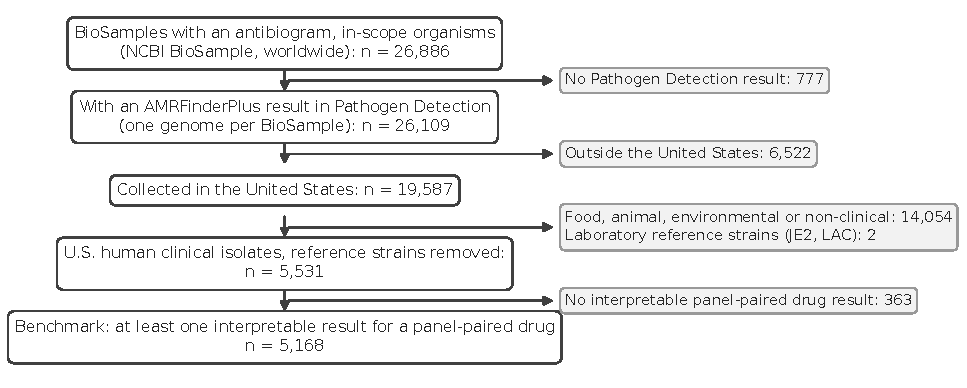
\includegraphics[width=0.86\textwidth]{figures/fig1_flow.pdf}
\caption{Construction of the benchmark from NCBI BioSample antibiograms and NCBI Pathogen Detection AMRFinderPlus results.
``Panel-paired drug'': a drug scored against a panel target for that organism (Table~\ref{tab:pairs}).}
\label{fig:flow}
\end{figure*}

\begin{table}[t]
\caption{Benchmark isolates by organism group.}
\label{tab:cohort}
\centering\footnotesize
\resizebox{\linewidth}{!}{\begin{tabular}{lrrrcrr}
\hline\hline
Organism & Isolates & Blood/sterile & Urine & Years & States$^{a}$ & BioProjects \\
\hline
\textit{E.~coli} & 3{,}176 & 314 & 2{,}636 & 2012--2024 & 7 & 39 \\
\textit{K.~pneumoniae} cplx. & 790 & 83 & 494 & 2003--2024 & 22 & 72 \\
\textit{S.~aureus} & 550 & 260 & 18 & 2011--2024 & 5 & 7 \\
\textit{E.~cloacae} cplx. & 166 & 13 & 82 & 2012--2024 & 2 & 21 \\
\textit{K.~aerogenes} & 115 & 11 & 64 & 2011--2024 & 5 & 17 \\
\textit{Salmonella enterica} & 109 & 9 & 8 & 2012--2017 & 2 & 4 \\
\textit{E.~faecalis} & 83 & 7 & 55 & 2016--2023 & 2 & 2 \\
\textit{C.~freundii} cplx. & 54 & 9 & 26 & 2012--2024 & 3 & 5 \\
\textit{E.~faecium} & 36 & 12 & 13 & 2016--2024 & 3 & 3 \\
\textit{Morganella}/\textit{Providencia} & 31 & 3 & 14 & 2014--2024 & 1 & 4 \\
\textit{Serratia} spp. & 30 & 4 & 4 & 2013--2024 & 1 & 3 \\
\textit{K.~oxytoca} cplx. & 18 & 6 & 6 & 2017--2024 & 2 & 2 \\
Other Enterobacterales & 7 & 0 & 3 & 2021--2023 & 1 & 1 \\
\textit{Klebsiella}, other & 3 & 0 & 3 & 2023--2024 & 1 & 1 \\
\hline
Total & 5{,}168 & 731 & 3{,}426 & 2003--2024 & 24 & 152 \\
\hline\hline
\end{tabular}
}
\par\vspace{2pt}\parbox{0.97\linewidth}{\footnotesize $^{a}$Distinct states named, District of Columbia included; isolates
without a stated location are not counted.}
\end{table}

\begin{figure*}[t]
\centering
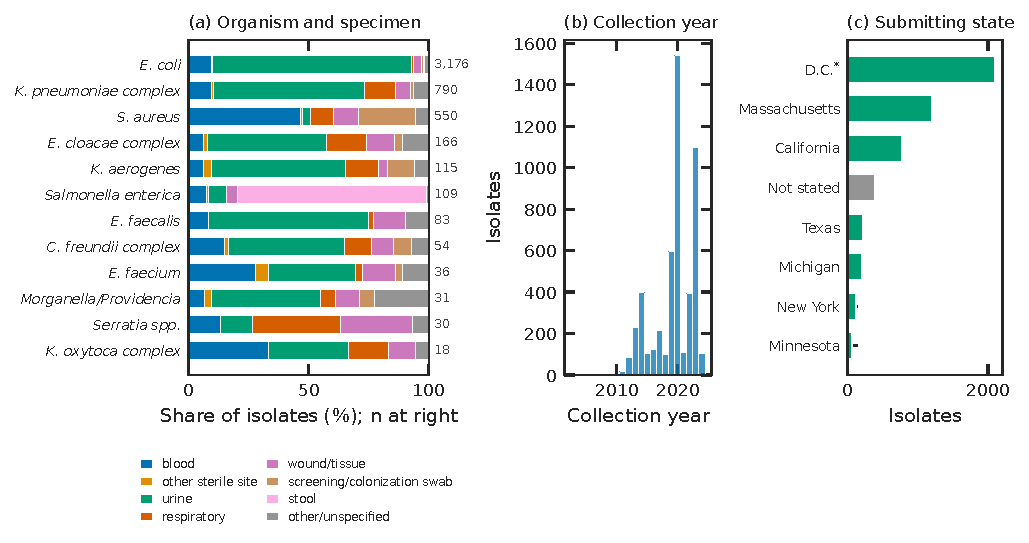
\includegraphics[width=\textwidth]{figures/fig2_cohort.pdf}
\caption{Benchmark composition. (a) Specimen category by organism group (groups with at least 10 isolates; totals at
right). (b) Collection year. (c) Submitting state, eight most frequent. $^{*}$All District of Columbia isolates were
submitted by the Walter Reed Army Institute of Research; the location is the submitter's.}
\label{fig:cohort}
\end{figure*}

\subsection{Panel targets detected}

AMRFinderPlus detected \g{mecA} in \nv{det-meca} isolates, \g{vanA} in \nv{det-vana}, KPC in \nv{det-kpc}, NDM in
\nv{det-ndm}, OXA-48-like enzymes in \nv{det-oxa48like}, VIM in \nv{det-vim}, IMP in \nv{det-imp} and CTX-M in
\nv{det-ctxm}; \g{mecC} and \g{vanB} were not found (Table~\ref{tab:xw}). \nv{n-any-carba} isolates carried at least one
panel carbapenemase, \nv{n-carba-kp} of them \kpn{} complex, and \nv{n-multi-carba} carried two or more. KPC-3
(\nv{kpc3}) and KPC-2 (\nv{kpc2}) dominated the KPC calls; NDM-1 (\nv{ndm1}) and NDM-5 (\nv{ndm5}) the NDM calls; and
OXA-181 (\nv{oxa181}), OXA-232 (\nv{oxa232}) and OXA-48 (\nv{oxa48}) the OXA-48-like calls. CTX-M-15 (\nv{ctxm15}),
CTX-M-27 (\nv{ctxm27}) and CTX-M-14 (\nv{ctxm14}) were the commonest CTX-M alleles. Only \nv{partial-ctxm} CTX-M calls,
and no other panel target calls, were partial.

\begin{table*}[t]
\caption{Gene-to-panel target crosswalk (AMRFinderPlus Reference Gene Hierarchy, database \nv{refgene-db}) and alleles
observed in the benchmark. ``Symbols'': crosswalk rows; ``Isolates'': benchmark isolates with the target detected.
An isolate carrying two alleles of one family counts once for each allele.}
\label{tab:xw}
\centering\footnotesize
\begin{tabular}{llrrrp{0.36\linewidth}}
\hline\hline
Target & Hierarchy node & Symbols & Non-carba.$^{a}$ & Isolates & Most frequent observed alleles (isolates) \\
\hline
mecA & \texttt{mecA} & 2 & -- & 220 & mecA (220) \\
mecC & \texttt{mecC} & 1 & -- & 0 & none \\
vanA & \texttt{vanA} & 1 & -- & 29 & vanA (29) \\
vanB & \texttt{vanB} & 1 & -- & 0 & none \\
KPC & \texttt{blaKPC} & 296 & -- & 209 & KPC-3 (130), KPC-2 (60), KPC-4 (17), KPC-82 (1) \\
NDM & \texttt{blaNDM} & 99 & -- & 41 & NDM-1 (23), NDM-5 (13), NDM-7 (3), NDM-4 (1) \\
OXA-48-like & \texttt{blaOXA-48\_fam} & 83 & 54 & 38 & OXA-181 (17), OXA-232 (11), OXA-48 (8), OXA-244 (1) \\
VIM & \texttt{blaVIM} & 97 & -- & 5 & VIM-1 (2), VIM-2 (2), VIM-4 (1) \\
IMP & \texttt{blaIMP} & 109 & -- & 8 & IMP-13 (4), IMP-27 (2), IMP-18 (1), IMP-67 (1) \\
CTX-M & \texttt{blaCTX-M} & 275 & -- & 1064 & CTX-M-15 (726), CTX-M-27 (182), CTX-M-14 (64), CTX-M-55 (54) \\
\hline\hline
\end{tabular}

\par\vspace{2pt}\parbox{0.9\textwidth}{\footnotesize $^{a}$OXA-48 family alleles that NCBI's catalog does not list as
carbapenem-hydrolyzing (flag \texttt{FAMILY\_MEMBER\_NONCARBA}).}
\end{table*}

\subsection{Main concordance results}

Table~\ref{tab:main} and Fig.~\ref{fig:forest} give the headline estimates; the full table of
\nv{n-concordance-rows} analysis rows is released with the data.

\begin{table*}[t]
\caption{Concordance of panel targets with laboratory susceptibility, all U.S. human clinical isolates (main analysis:
I and SDD counted as not resistant). G+R: gene detected, resistant; G+S: gene detected, not resistant; G$-$R: gene not
detected, resistant; G$-$S: gene not detected, not resistant. OXA, oxacillin; FOX, cefoxitin; VAN, vancomycin; CBP,
carbapenem; MEM, meropenem; CRO, ceftriaxone.}
\label{tab:main}
\centering\scriptsize
\resizebox{\textwidth}{!}{\begin{tabular}{lllrrrrrllrr}
\hline\hline
Target & Organism & Drug & $n$ & G+R & G+S & G$-$R & G$-$S & PPV (95\% CI) & NPV (95\% CI) & Sens. & Spec. \\
\hline
\textit{mecA} & \textit{S.~aureus} & OXA or FOX & 550 & 215 & 5 & 1 & 329 & 97.7\% (94.8\%--99.0\%) & 99.7\% (98.3\%--99.9\%) & 99.5\% & 98.5\% \\
\textit{mecA} & \textit{S.~aureus} & OXA & 550 & 215 & 5 & 0 & 330 & 97.7\% (94.8\%--99.0\%) & 100.0\% (98.8\%--100.0\%) & 100.0\% & 98.5\% \\
\textit{vanA} & \textit{E.~faecium} & VAN & 36 & 22 & 3 & 1 & 10 & 88.0\% (70.0\%--95.8\%) & 90.9\% (62.3\%--98.4\%) & 95.7\% & 76.9\% \\
\textit{vanA} & \textit{E.~faecalis} & VAN & 83 & 4 & 0 & 2 & 77 & 100.0\% (51.0\%--100.0\%) & 97.5\% (91.2\%--99.3\%) & 66.7\% & 100.0\% \\
\textit{vanA}/\textit{vanB} & \textit{E.~faecalis} + \textit{E.~faecium} & VAN & 119 & 26 & 3 & 3 & 87 & 89.7\% (73.6\%--96.4\%) & 96.7\% (90.7\%--98.9\%) & 89.7\% & 96.7\% \\
KPC & Enterobacterales$^{a}$ & Any CBP & 4{,}147 & 199 & 4 & 224 & 3{,}720 & 98.0\% (95.0\%--99.2\%) & 94.3\% (93.6\%--95.0\%) & 47.0\% & 99.9\% \\
NDM & Enterobacterales$^{a}$ & Any CBP & 4{,}147 & 41 & 0 & 382 & 3{,}724 & 100.0\% (91.4\%--100.0\%) & 90.7\% (89.8\%--91.5\%) & 9.7\% & 100.0\% \\
OXA-48-like & Enterobacterales$^{a}$ & Any CBP & 4{,}147 & 36 & 2 & 387 & 3{,}722 & 94.7\% (82.7\%--98.5\%) & 90.6\% (89.7\%--91.4\%) & 8.5\% & 99.95\% \\
VIM & Enterobacterales$^{a}$ & Any CBP & 4{,}147 & 5 & 0 & 418 & 3{,}724 & 100.0\% (56.6\%--100.0\%) & 89.9\% (89.0\%--90.8\%) & 1.2\% & 100.0\% \\
IMP & Enterobacterales$^{a}$ & Any CBP & 4{,}147 & 8 & 0 & 415 & 3{,}724 & 100.0\% (67.6\%--100.0\%) & 90.0\% (89.0\%--90.9\%) & 1.9\% & 100.0\% \\
Any carbapenemase$^{b}$ & Enterobacterales$^{a}$ & Any CBP & 4{,}147 & 272 & 6 & 151 & 3{,}718 & 97.8\% (95.4\%--99.0\%) & 96.1\% (95.4\%--96.7\%) & 64.3\% & 99.8\% \\
Any carbapenemase$^{b}$ & Enterobacterales$^{a}$ & MEM & 3{,}834 & 241 & 34 & 88 & 3{,}471 & 87.6\% (83.2\%--91.0\%) & 97.5\% (97.0\%--98.0\%) & 73.2\% & 99.0\% \\
CTX-M & \textit{E.~coli} & CRO & 2{,}828 & 654 & 19 & 124 & 2{,}031 & 97.2\% (95.6\%--98.2\%) & 94.2\% (93.2\%--95.2\%) & 84.1\% & 99.1\% \\
CTX-M & \textit{K.~pneumoniae} cplx. & CRO & 636 & 216 & 2 & 262 & 156 & 99.1\% (96.7\%--99.7\%) & 37.3\% (32.8\%--42.1\%) & 45.2\% & 98.7\% \\
CTX-M & Enterobacterales$^{a}$ & CRO & 3{,}855 & 905 & 21 & 696 & 2{,}233 & 97.7\% (96.6\%--98.5\%) & 76.2\% (74.7\%--77.7\%) & 56.5\% & 99.1\% \\
CTX-M & \textit{Salmonella enterica} & CRO & 108 & 1 & 0 & 14 & 93 & 100.0\% (20.7\%--100.0\%) & 86.9\% (79.2\%--92.0\%) & 6.7\% & 100.0\% \\
\hline\hline
\end{tabular}
}
\par\vspace{2pt}\parbox{\textwidth}{\footnotesize $^{a}$Pooled Enterobacterales excluding \textit{Salmonella}.
$^{b}$KPC, NDM, OXA-48-like, VIM or IMP.}
\end{table*}

\begin{figure*}[t]
\centering
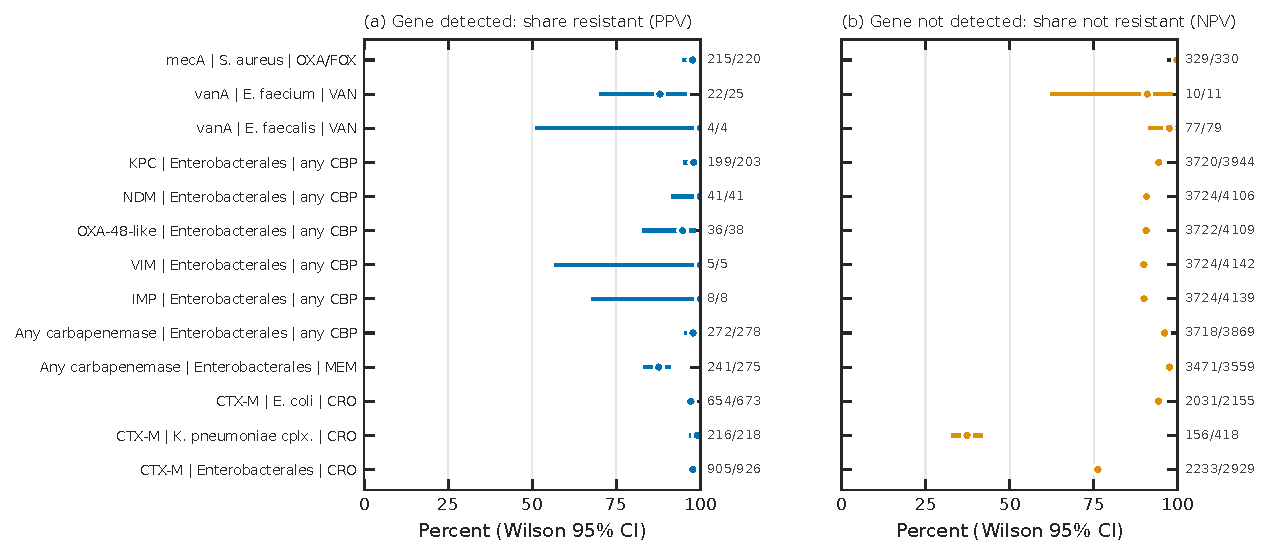
\includegraphics[width=\textwidth]{figures/fig3_forest.pdf}
\caption{Positive (a) and negative (b) predictive values with Wilson 95\% confidence intervals for the principal
target--organism--drug combinations. Fractions at right are the counts behind each estimate. ``Enterobacterales'' excludes
\textit{Salmonella}. CBP, carbapenem; MEM, meropenem; CRO, ceftriaxone; OXA/FOX, oxacillin or cefoxitin; VAN,
vancomycin.}
\label{fig:forest}
\end{figure*}

\subsubsection{\g{mecA} and \g{mecC} in \sau{}}
\g{mecA} was detected in \nv{meca-genepos} of \nv{meca-n} \sau{} with an oxacillin or cefoxitin result, and
\nv{meca-geneposR} of them were resistant (PPV \nv{meca-ppv}, 95\% CI \nv{meca-ppv-ci}). Among isolates without \g{mecA}
or \g{mecC}, \nv{mecamecc-npv-frac} were not resistant (NPV \nv{mecamecc-npv}, \nv{mecamecc-npv-ci}); sensitivity was
\nv{meca-sensitivity} and specificity \nv{meca-specificity}. The phenotype separated cleanly by genotype
(Fig.~\ref{fig:mic}a): almost every \g{mecA}-negative isolate had an oxacillin MIC $\le$0.5~mg/L and almost every
\g{mecA}-positive isolate an MIC $\ge$4~mg/L. The \nv{gp-meca} \g{mecA}-positive isolates without resistance
(\nv{meca-s-ids}) had oxacillin MICs of 0.25 to 2~mg/L (Appendix Table~\ref{tab:app}); for \nv{mecaalt-n} of them the
submitting laboratory had nevertheless reported oxacillin resistance. One \g{mecA}-negative isolate
(\nv{gn-meca-ids}) was cefoxitin-resistant (MIC $\ge$64~mg/L) with an oxacillin MIC of 0.5~mg/L and no other \g{mec}
gene detected.

\subsubsection{\g{vanA} and \g{vanB} in enterococci}
The enterococcal arm is small. \g{vanA} was detected in \nv{van-genepos} of \nv{van-n} enterococci with a vancomycin
result, and \nv{van-geneposR} were resistant (PPV \nv{van-ppv}, \nv{van-ppv-ci}); NPV was \nv{van-npv}
(\nv{van-npv-ci}). In \textit{E.~faecium}, PPV was \nv{vana-fm-ppv} (\nv{vana-fm-ppv-frac}) and NPV \nv{vana-fm-npv}
(\nv{vana-fm-npv-frac}); in \textit{E.~faecalis} all \nv{vana-fs-genepos} \g{vanA}-positive isolates were resistant.
The \nv{gp-vana} \g{vanA}-positive, vancomycin-susceptible isolates were all \textit{E.~faecium} (\nv{vana-s-ids}) with
vancomycin MICs of 1 to 2~mg/L, a pattern described as vancomycin-variable or silent \g{vanA}
\cite{szakacs2014,vanA2025} (Fig.~\ref{fig:mic}b). Of the \nv{gn-van} vancomycin-resistant isolates without a panel
\g{van} gene, one carried \g{vanA} operon accessory genes (\g{vanY}, \g{vanZ}) without a ligase call, suggesting an
assembly break, and two \textit{E.~faecalis} had no explanation in the available data.

\subsubsection{Carbapenemases in Enterobacterales}
Any panel carbapenemase predicted resistance to at least one carbapenem in \nv{carb-any-ppv-frac} isolates (PPV
\nv{carb-any-ppv}, \nv{carb-any-ppv-ci}); its absence predicted no carbapenem resistance in \nv{carb-any-npv-frac}
(NPV \nv{carb-any-npv}, \nv{carb-any-npv-ci}). Sensitivity was \nv{carb-any-sensitivity}: about a third of
carbapenem-resistant Enterobacterales in this collection carried none of the five panel enzymes. KPC alone had PPV
\nv{kpc-any-ppv} (\nv{kpc-any-ppv-frac}), NDM \nv{ndm-any-ppv} (\nv{ndm-any-ppv-frac}) and OXA-48-like \nv{oxa-any-ppv}
(\nv{oxa-any-ppv-frac}).

The predictive value of a carbapenemase depended on which carbapenem was asked about (Table~\ref{tab:carbdrug},
Fig.~\ref{fig:carbdrug}). Ertapenem resistance followed a carbapenemase in \nv{carb-erta-ppv} of tested producers, but meropenem resistance
did not:
for any panel carbapenemase, PPV was \nv{carb-mero-ppv} for meropenem (\nv{carb-mero-ppv-frac}) against
\nv{carb-erta-ppv} for ertapenem (\nv{carb-erta-ppv-frac}) and \nv{carb-imi-ppv} for imipenem. By enzyme, meropenem PPV
was \nv{enz-kpc-mero-pct} for KPC (\nv{enz-kpc-mero}), \nv{enz-ndm-mero-pct} for NDM (\nv{enz-ndm-mero}),
\nv{enz-oxa48like-mero-pct} for OXA-48-like (\nv{enz-oxa48like-mero}) and \nv{enz-imp-mero-pct} for IMP
(\nv{enz-imp-mero}). The meropenem MIC distribution of carbapenemase-positive isolates (Fig.~\ref{fig:mic}c) had a long
tail at and below the resistant breakpoint. Doripenem was tested in \nv{dori-n} isolates (median collection year \nv{dori-median-year}), mostly from
one project, and is shown for completeness.

By organism, PPV for any carbapenem was high in \kpn{} complex (\nv{carb-any-kp-ppv-frac}) and \textit{E.~cloacae} complex
(\nv{carb-any-ecl-ppv-frac}), but NPV fell where non-carbapenemase mechanisms are common: \nv{carb-any-ecl-npv} in
\textit{E.~cloacae} complex and \nv{carb-any-kae-npv} in \textit{K.~aerogenes} (Table~\ref{tab:carborg}). In \eco{},
carbapenemase-positive isolates were often meropenem-susceptible (meropenem PPV \nv{carb-mero-ec-ppv},
\nv{carb-mero-ec-ppv-frac}).

\begin{table}[t]
\caption{PPV of each carbapenemase for resistance to each carbapenem, pooled Enterobacterales excluding
\textit{Salmonella}: resistant / gene-positive tested (percent).}
\label{tab:carbdrug}
\centering\footnotesize
\resizebox{\linewidth}{!}{\begin{tabular}{lccccc}
\hline\hline
Target & Meropenem & Imipenem & Ertapenem & Doripenem & Any carbapenem \\
\hline
KPC & 182/201 (91\%) & 159/170 (94\%) & 161/166 (97\%) & 109/141 (77\%) & 199/203 (98\%) \\
NDM & 40/41 (98\%) & 16/16 (100\%) & 18/20 (90\%) & 6/6 (100\%) & 41/41 (100\%) \\
OXA-48-like & 29/38 (76\%) & 27/36 (75\%) & 31/32 (97\%) & 24/30 (80\%) & 36/38 (95\%) \\
VIM & 3/4 (75\%) & 4/4 (100\%) & 2/3 (67\%) & 0/1 (0\%) & 5/5 (100\%) \\
IMP & 3/8 (38\%) & 2/4 (50\%) & 5/5 (100\%) & -- & 8/8 (100\%) \\
Any panel enzyme & 241/275 (88\%) & 193/215 (90\%) & 213/222 (96\%) & 135/174 (78\%) & 272/278 (98\%) \\
\hline\hline
\end{tabular}
}
\end{table}

\begin{figure}[t]
\centering
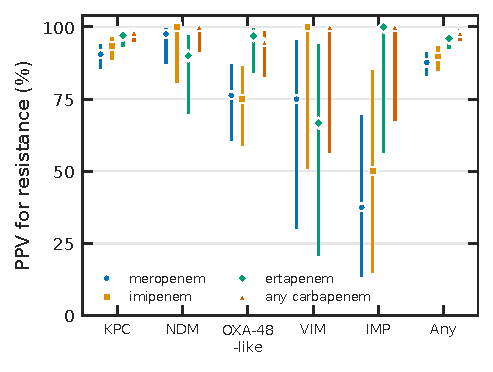
\includegraphics[width=\linewidth]{figures/fig4_carb_drug.pdf}
\caption{PPV of each panel carbapenemase for resistance to meropenem, imipenem, ertapenem and any carbapenem, pooled
Enterobacterales excluding \textit{Salmonella}, with Wilson 95\% CIs. ``Any'': any of the five panel enzymes.}
\label{fig:carbdrug}
\end{figure}

\begin{table}[t]
\caption{Any panel carbapenemase by organism group. PPV and NPV as resistant/gene-positive and not resistant/gene-negative.}
\label{tab:carborg}
\centering\footnotesize
\resizebox{\linewidth}{!}{\begin{tabular}{lrrllrll}
\hline\hline
 & \multicolumn{5}{c}{Any carbapenem} & \multicolumn{2}{c}{Meropenem} \\ \cline{2-6}\cline{7-8} Organism & $n$ & G+ & PPV & NPV & Sens. & PPV & NPV \\
\hline
\textit{E.~coli} & 3{,}168 & 29 & 26/29 & 3102/3139 & 41.3\% & 17/29 & 2871/2889 \\
\textit{K.~pneumoniae} cplx. & 564 & 186 & 185/186 & 339/378 & 82.6\% & 177/185 & 289/320 \\
\textit{E.~cloacae} cplx. & 163 & 37 & 37/37 & 104/126 & 62.7\% & 29/36 & 116/124 \\
\textit{K.~aerogenes} & 110 & 4 & 4/4 & 61/106 & 8.2\% & 3/4 & 81/106 \\
\textit{C.~freundii} cplx. & 54 & 7 & 6/7 & 46/47 & 85.7\% & 5/7 & 46/47 \\
\textit{Serratia} spp. & 29 & 3 & 3/3 & 22/26 & 42.9\% & 2/2 & 23/26 \\
\textit{Morganella}/\textit{Providencia} & 31 & 5 & 4/5 & 24/26 & 66.7\% & 2/5 & 24/26 \\
Enterobacterales$^{a}$ & 4{,}147 & 278 & 272/278 & 3718/3869 & 64.3\% & 241/275 & 3471/3559 \\
\hline\hline
\end{tabular}
}
\end{table}

\subsubsection{CTX-M and third-generation cephalosporins}
CTX-M predicted ceftriaxone resistance with PPV \nv{ctx-cro-ppv} (\nv{ctx-cro-ppv-ci}) in pooled Enterobacterales,
\nv{ctx-cro-ec-ppv} in \eco{} and \nv{ctx-cro-kp-ppv} in \kpn{} complex (Table~\ref{tab:ctxorg}). The value of a negative
result depended strongly on organism (Fig.~\ref{fig:ctxm}a). In \eco{}, \nv{ctx-cro-ec-npv-frac} CTX-M-negative isolates
were not ceftriaxone-resistant (NPV \nv{ctx-cro-ec-npv}); in \kpn{} complex only \nv{ctx-cro-kp-npv-frac} were (NPV
\nv{ctx-cro-kp-npv}), because most CTX-M-negative, ceftriaxone-resistant \kpn{} carried another acquired ESBL or AmpC
(\nv{kp-ctx-gn-acq} of \nv{kp-ctx-gn} as primary cause, mostly SHV-type) or a panel carbapenemase
(\nv{kp-ctx-gn-carb}). In chromosomal AmpC
species the NPV was below 10\%: \nv{ctx-cro-ecl-npv} in \textit{E.~cloacae} complex, \nv{ctx-cro-kae-npv} in
\textit{K.~aerogenes} and \nv{ctx-cro-cf-npv} in \textit{C.~freundii} complex. For \textit{Salmonella}, CTX-M was rare
and the NPV was \nv{ctx-cro-sal-npv}.

CTX-M predicted ceftazidime resistance much less reliably than ceftriaxone resistance (PPV \nv{ctx-caz-ec-ppv} in
\eco{}, \nv{ctx-caz-kp-ppv} in \kpn{} complex). The secondary analysis attributes this to the CTX-M subgroup
(Table~\ref{tab:ctxsub}, Fig.~\ref{fig:ctxm}b). In \eco{}, CTX-M-1-group enzymes conferred ceftriaxone resistance in
\nv{sub-ecg1-ceftri} (\nv{sub-ecg1-ceftri-pct}) and ceftazidime resistance in \nv{sub-ecg1-ceftaz}
(\nv{sub-ecg1-ceftaz-pct}); CTX-M-9-group enzymes conferred ceftriaxone resistance in \nv{sub-ecg9-ceftri}
(\nv{sub-ecg9-ceftri-pct}) but ceftazidime resistance in only \nv{sub-ecg9-ceftaz} (\nv{sub-ecg9-ceftaz-pct};
Fisher exact \nv{sub-ec-fisher}). In \kpn{} complex, CTX-M-1-group enzymes conferred ceftazidime resistance in
\nv{sub-kpg1-ceftaz} (\nv{sub-kpg1-ceftaz-pct}); CTX-M-9-group enzymes were too few to compare.

\begin{table}[t]
\caption{CTX-M and ceftriaxone by organism group.}
\label{tab:ctxorg}
\centering\footnotesize
\resizebox{\linewidth}{!}{\begin{tabular}{lrrllrr}
\hline\hline
Organism & $n$ & CTX-M+ & PPV (95\% CI) & NPV (95\% CI) & Sens. & Spec. \\
\hline
\textit{E.~coli} & 2{,}828 & 673 & 97.2\% (95.6\%--98.2\%) & 94.2\% (93.2\%--95.2\%) & 84.1\% & 99.1\% \\
\textit{K.~pneumoniae} cplx. & 636 & 218 & 99.1\% (96.7\%--99.7\%) & 37.3\% (32.8\%--42.1\%) & 45.2\% & 98.7\% \\
\textit{K.~oxytoca} cplx. & 18 & 7 & 100.0\% (64.6\%--100.0\%) & 18.2\% (5.1\%--47.7\%) & 43.8\% & 100.0\% \\
\textit{E.~cloacae} cplx. & 149 & 12 & 100.0\% (75.8\%--100.0\%) & 4.4\% (2.0\%--9.2\%) & 8.4\% & 100.0\% \\
\textit{K.~aerogenes} & 103 & 3 & 100.0\% (43.9\%--100.0\%) & 7.0\% (3.4\%--13.7\%) & 3.1\% & 100.0\% \\
\textit{C.~freundii} cplx. & 52 & 1 & 100.0\% (20.7\%--100.0\%) & 7.8\% (3.1\%--18.5\%) & 2.1\% & 100.0\% \\
\textit{Serratia} spp. & 30 & 0 & -- & 63.3\% (45.5\%--78.1\%) & 0.0\% & 100.0\% \\
\textit{Morganella}/\textit{Providencia} & 29 & 4 & 100.0\% (51.0\%--100.0\%) & 32.0\% (17.2\%--51.6\%) & 19.1\% & 100.0\% \\
\textit{Salmonella enterica} & 108 & 1 & 100.0\% (20.7\%--100.0\%) & 86.9\% (79.2\%--92.0\%) & 6.7\% & 100.0\% \\
Enterobacterales$^{a}$ & 3{,}855 & 926 & 97.7\% (96.6\%--98.5\%) & 76.2\% (74.7\%--77.7\%) & 56.5\% & 99.1\% \\
\hline\hline
\end{tabular}
}
\par\vspace{2pt}\parbox{0.97\linewidth}{\footnotesize $^{a}$Excluding \textit{Salmonella}.}
\end{table}

\begin{figure*}[t]
\centering
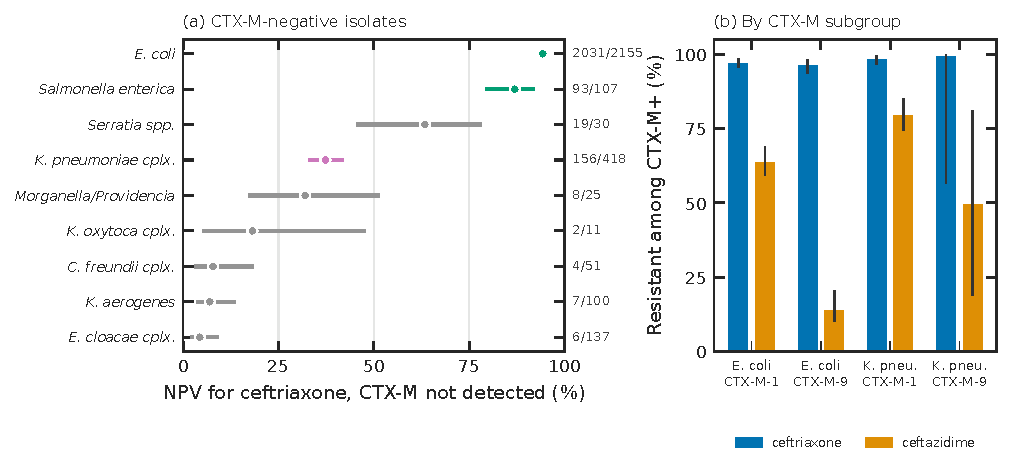
\includegraphics[width=\textwidth]{figures/fig5_ctxm.pdf}
\caption{CTX-M and third-generation cephalosporins. (a) NPV of a CTX-M-negative result for ceftriaxone by organism group
(Wilson 95\% CI; green, \eco{} and \textit{Salmonella}; purple, \kpn{} complex; gray, species with chromosomal AmpC or
other intrinsic cephalosporinases). (b) Share resistant to ceftriaxone and ceftazidime among CTX-M-positive isolates, by
CTX-M subgroup (CTX-M-1 group, e.g. CTX-M-15, -55; CTX-M-9 group, e.g. CTX-M-14, -27).}
\label{fig:ctxm}
\end{figure*}

\begin{table}[t]
\caption{Secondary analysis: third-generation cephalosporin resistance among CTX-M-positive isolates by CTX-M subgroup
(resistant/tested, percent). Isolates carrying both subgroups or untyped CTX-M are not shown.}
\label{tab:ctxsub}
\centering\footnotesize
\resizebox{\linewidth}{!}{\begin{tabular}{llccc}
\hline\hline
Organism & CTX-M subgroup & Ceftriaxone R & Cefotaxime R & Ceftazidime R \\
\hline
\textit{E.~coli} & CTX-M-1 group & 432/443 (98\%) & 21/21 (100\%) & 235/366 (64\%) \\
\textit{E.~coli} & CTX-M-9 group & 211/218 (97\%) & 5/5 (100\%) & 26/179 (15\%) \\
\textit{K.~pneumoniae} cplx. & CTX-M-1 group & 206/208 (99\%) & 72/72 (100\%) & 170/212 (80\%) \\
\textit{K.~pneumoniae} cplx. & CTX-M-9 group & 5/5 (100\%) & 4/4 (100\%) & 3/6 (50\%) \\
\hline\hline
\end{tabular}
}
\end{table}

\begin{figure*}[t]
\centering
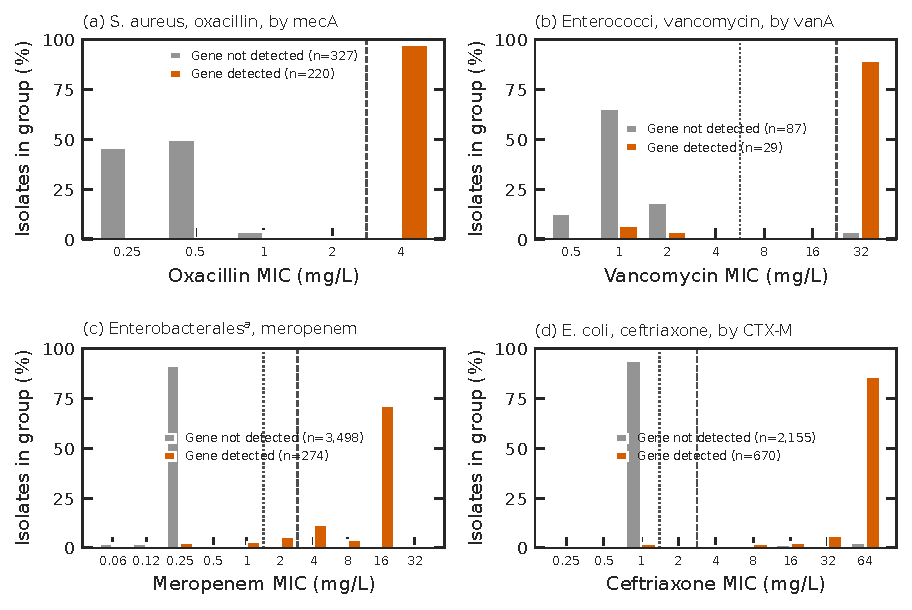
\includegraphics[width=\textwidth]{figures/fig6_mic.pdf}
\caption{MIC distributions by panel-target status. Bars show the share of isolates in each group at each MIC on the
two-fold scale; censored readings are placed at their bound ($\le x$ and $\ge x$ at $x$, $<x$ at $x/2$, $>x$ at $2x$) and
gradient-strip half-steps are rounded up. Dotted line: susceptible breakpoint; dashed line: resistant breakpoint
(CLSI M100-Ed35). (a) \sau{}, oxacillin, by \g{mecA}. (b) Enterococci, vancomycin, by \g{vanA}. (c) Enterobacterales
excluding \textit{Salmonella}$^{a}$, meropenem, by any panel carbapenemase. (d) \eco{}, ceftriaxone, by CTX-M.}
\label{fig:mic}
\end{figure*}

\subsection{Sensitivity analyses}

The headline estimates were stable when I and SDD results were excluded instead of counted as not resistant
(Table~\ref{tab:sens}, Fig.~\ref{fig:robust}). Excluding them raised the meropenem PPV of any panel carbapenemase from
\nv{carb-mero-ppv} to \nv{carb-mero-exI-ppv}, because many carbapenemase producers have meropenem MICs in the
intermediate range. Restricting to blood and sterile-site isolates left the \g{mecA} and carbapenemase estimates within
the confidence intervals of the main analysis, with wider intervals; the NPV of CTX-M for ceftriaxone in \eco{} was lower
in blood isolates (\nv{ctx-cro-ec-blood-npv}, \nv{ctx-cro-ec-blood-npv-frac}) than overall (\nv{ctx-cro-ec-npv}).
Accepting the submitting laboratory's oxacillin call for \sau{} raised the \g{mecA} PPV from \nv{meca-ppv} to
\nv{mecaalt-ppv} (\nv{mecaalt-frac}).

\begin{table*}[t]
\caption{Sensitivity analyses for the headline estimates.}
\label{tab:sens}
\centering\footnotesize
\begin{tabular}{lrrrrrrrrr}
\hline\hline
 & \multicolumn{3}{c}{Main analysis} & \multicolumn{3}{c}{I/SDD excluded} & \multicolumn{3}{c}{Blood/sterile site} \\ \cline{2-4}\cline{5-7}\cline{8-10} Analysis & $n$ & PPV & NPV & $n$ & PPV & NPV & $n$ & PPV & NPV \\
\hline
\textit{mecA}, \textit{S.~aureus}, OXA/FOX & 550 & 97.7\% & 99.7\% & 550 & 97.7\% & 99.7\% & 260 & 98.7\% & 100.0\% \\
\textit{vanA}/\textit{B}, enterococci, VAN & 119 & 89.7\% & 96.7\% & 119 & 89.7\% & 96.7\% & 19 & 77.8\% & 100.0\% \\
KPC, Enterobacterales, any CBP & 4{,}147 & 98.0\% & 94.3\% & 4{,}101 & 99.5\% & 94.3\% & 420 & 100.0\% & 93.6\% \\
Any carbapenemase, any CBP & 4{,}147 & 97.8\% & 96.1\% & 4{,}101 & 98.9\% & 96.0\% & 420 & 97.3\% & 95.0\% \\
Any carbapenemase, MEM & 3{,}834 & 87.6\% & 97.5\% & 3{,}793 & 93.4\% & 97.5\% & 420 & 86.5\% & 97.1\% \\
CTX-M, \textit{E.~coli}, CRO & 2{,}828 & 97.2\% & 94.2\% & 2{,}825 & 97.5\% & 94.2\% & 262 & 98.5\% & 80.5\% \\
CTX-M, \textit{K.~pneumoniae} cplx., CRO & 636 & 99.1\% & 37.3\% & 601 & 99.1\% & 31.6\% & 63 & 94.4\% & 28.9\% \\
\hline\hline
\end{tabular}

\end{table*}

\begin{figure*}[t]
\centering
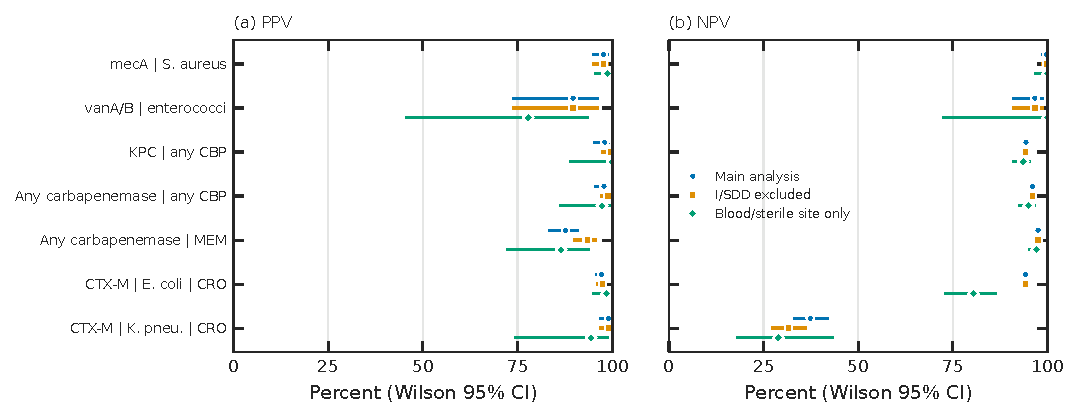
\includegraphics[width=\textwidth]{figures/fig8_robustness.pdf}
\caption{Robustness of PPV (a) and NPV (b) to excluding intermediate and SDD results and to restricting to blood and
sterile-site isolates, with Wilson 95\% CIs. CBP, carbapenem; MEM, meropenem; CRO, ceftriaxone.}
\label{fig:robust}
\end{figure*}

\subsection{Discordant isolates}

The discordance collection contains \nv{n-discordance-cases} isolate-target pairs from \nv{n-discordant-isolates}
isolates: \nv{disc-gp} with the gene detected but no resistance, and \nv{disc-gn} resistant without the panel target
(Table~\ref{tab:disc}, Fig.~\ref{fig:disc}).

Gene-detected, not-resistant isolates were few. Of the \nv{disc-gp}, \nv{gp-near} had a measured value at or within
one dilution of the resistant breakpoint, \nv{gp-subdiff} had a submitter call that differed from our reinterpretation,
and \nv{gp-unexpl} had no explanation in the available data (Appendix Table~\ref{tab:app}). For \sau{}, in
\nv{mecaalt-n} of the \nv{gp-meca} cases the submitting laboratory had reported oxacillin resistance despite the MIC. No
gene-detected, not-resistant case involved a partial gene call.

Gene-negative resistant isolates were dominated by third-generation cephalosporin resistance without CTX-M
(\nv{disc-ceph-gn} of \nv{disc-gn}). Of these, \nv{dc-ceph-gn-acqesbl} carried an acquired non-CTX-M ESBL or AmpC,
\nv{dc-ceph-gn-ampcorg} belonged to a species with chromosomal AmpC, and \nv{dc-ceph-gn-carbpres} carried a panel
carbapenemase, which itself confers cephalosporin resistance; \nv{dc-ceph-gn-unexpl} were unexplained. Among
\nv{disc-carb-gn} carbapenem-resistant isolates without a panel carbapenemase, \nv{dc-carb-gn-esblporin} carried an ESBL or
AmpC with a porin change, \nv{dc-carb-gn-esblnoporin} an ESBL or AmpC without a called porin change, and
\nv{dc-carb-gn-poriononly} a porin change alone, consistent with non-carbapenemase carbapenem resistance
\cite{tamma2017,pitout2015}; \nv{dc-carb-gn-near} had a value within one dilution of the breakpoint, and
\nv{dc-carb-gn-npcarb} carried a non-panel carbapenemase (\nv{npc-genes}).

\begin{table}[t]
\caption{Discordant isolate-target pairs by primary cause and drug class.}
\label{tab:disc}
\centering\footnotesize
\resizebox{\linewidth}{!}{\begin{tabular}{lrrrrr}
\hline\hline
Primary cause & Methicillin & Vancomycin & Carbapenem & 3GC$^{a}$ & Total \\
\hline
\multicolumn{6}{l}{\textit{Gene detected, not resistant}} \\
\quad Unexplained by available data & 1 & 3 & 3 & 21 & 28 \\
\quad MIC within one dilution of R breakpoint & 2 & -- & 3 & 2 & 7 \\
\quad Submitter call differs from M100-Ed35 & 2 & -- & -- & -- & 2 \\
\quad \textit{Subtotal} & 5 & 3 & 6 & 23 & 37 \\
\hline
\multicolumn{6}{l}{\textit{Gene not detected, resistant}} \\
\quad Acquired non-CTX-M ESBL or AmpC & -- & -- & -- & 268 & 268 \\
\quad Chromosomal AmpC organism & -- & -- & -- & 254 & 254 \\
\quad Panel carbapenemase present & -- & -- & -- & 201 & 201 \\
\quad MIC within one dilution of R breakpoint & -- & -- & 36 & 23 & 59 \\
\quad Unexplained by available data & 1 & 2 & 23 & 31 & 57 \\
\quad ESBL/AmpC, no porin call & -- & -- & 44 & -- & 44 \\
\quad Porin change only & -- & -- & 31 & -- & 31 \\
\quad ESBL/AmpC plus porin change & -- & -- & 14 & -- & 14 \\
\quad Non-panel carbapenemase & -- & -- & 3 & -- & 3 \\
\quad Submitter call differs from M100-Ed35 & -- & -- & -- & 1 & 1 \\
\quad \textit{vanA} operon, no ligase call & -- & 1 & -- & -- & 1 \\
\quad \textit{Subtotal} & 1 & 3 & 151 & 778 & 933 \\
\hline\hline
\end{tabular}
}
\par\vspace{2pt}\parbox{0.97\linewidth}{\footnotesize $^{a}$Third-generation cephalosporins.}
\end{table}

\begin{figure*}[t]
\centering
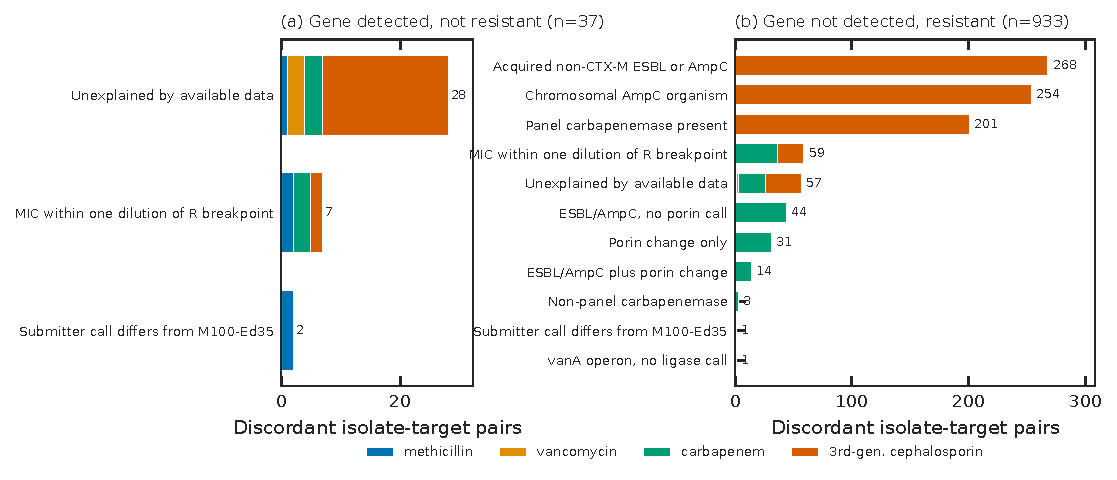
\includegraphics[width=\textwidth]{figures/fig7_discordance.pdf}
\caption{Discordant isolate-target pairs by primary cause, colored by drug class. (a) Gene detected, not resistant.
(b) Gene not detected, resistant. Causes are rule-based likely causes, not proven mechanisms.}
\label{fig:disc}
\end{figure*}

% ============================================================================
\section{Discussion}\label{sec:discussion}

\subsection{Principal findings}

Using public data alone, this benchmark measures how well the resistance targets on rapid blood culture panels predict
the susceptibility result that follows, for \nv{n-benchmark-isolates} U.S. clinical isolates. Three patterns stand out.
First, a \emph{detected} target was a strong signal for most combinations: \g{mecA} for oxacillin or cefoxitin in \sau{}
(\nv{meca-ppv}), KPC and NDM for any carbapenem (\nv{kpc-any-ppv} and \nv{ndm-any-ppv}), and CTX-M for ceftriaxone
(\nv{ctx-cro-ppv}) all had PPVs above 97\%. Second, a \emph{negative} result was organism-dependent:
excellent for \g{mecA} in \sau{} and good for CTX-M in \eco{}, but weak for CTX-M in \kpn{} and nearly uninformative in
chromosomal AmpC species. Third, the drug matters as much as the gene: carbapenemase producers were almost always
ertapenem-resistant but often meropenem-susceptible, and CTX-M-9-group producers were usually ceftazidime-susceptible.

\subsection{Interpretation by target}

\subsubsection{\g{mecA}}
The near-complete separation of oxacillin MICs by \g{mecA} status agrees with earlier genome-based studies of \sau{}
\cite{gordon2014}. The \g{mecA}-positive, oxacillin-susceptible isolates resemble oxacillin-susceptible MRSA, which can be
missed by phenotypic testing \cite{osmrsa2002}. Because CLSI directs that \sau{} positive for \g{mecA} or PBP2a be reported
as oxacillin-resistant \cite{clsi2025}, the laboratory call and the MIC can legitimately differ; we kept the MIC to avoid
circularity and report both.

\subsubsection{\g{vanA}}
The \g{vanA}-positive, vancomycin-susceptible \textit{E.~faecium} are consistent with vancomycin-variable enterococci,
which can revert to resistance under glycopeptide exposure \cite{szakacs2014,vanA2025}. For a panel result this means
that a positive \g{vanA} should not be over-ruled by an early susceptible phenotype. The enterococcal sample is small, and
the absence of \g{vanB} means this release cannot estimate \g{vanB} performance.

\subsubsection{Carbapenemases}
High PPV for ``any carbapenem'' coexisted with lower PPV for meropenem. OXA-48-like enzymes hydrolyze carbapenems weakly
and often leave meropenem MICs below the resistant breakpoint \cite{poirel2012}. The same pattern was common for IMP
(only \nv{enz-imp-mero} meropenem-resistant) and less common for KPC (\nv{enz-kpc-mero}). Treatment guidance distinguishes carbapenemase producers by enzyme class rather than by meropenem MIC
\cite{idsa2024}, so a carbapenemase-positive, meropenem-susceptible isolate is not a panel error but a reason to report
enzyme and MIC together. Conversely, about a third of carbapenem-resistant isolates had no panel carbapenemase, most with an
ESBL or AmpC and porin change; non-carbapenemase carbapenem-resistant Enterobacterales differ clinically from
carbapenemase producers \cite{tamma2017}. A negative carbapenemase panel therefore rules out the five enzymes, not carbapenem
resistance, particularly in \textit{Enterobacter} and \textit{K.~aerogenes}.

\subsubsection{CTX-M}
The weak NPV of CTX-M outside \eco{} reflects well-known biology: SHV- and TEM-type ESBLs and plasmid AmpC in \kpn{}
\cite{bush2020}, and chromosomal AmpC in \textit{Enterobacter}, \textit{K.~aerogenes} and \textit{Citrobacter}
\cite{jacoby2009}. The subgroup analysis shows that CTX-M is not one phenotype: CTX-M-15 and related CTX-M-1-group enzymes
commonly confer ceftazidime resistance, whereas CTX-M-14 and CTX-M-27 usually do not; together these two were the second and third
commonest CTX-M alleles in this collection (CTX-M-27 in \nv{ctxm27} isolates and CTX-M-14 in \nv{ctxm14}), consistent with the spread of CTX-M-27
described elsewhere \cite{bevan2017}. Panels report ``CTX-M'' without the subgroup, so a CTX-M result predicts ceftriaxone resistance far better
than ceftazidime resistance.

\subsection{Implications}

These estimates can inform how laboratories word panel reports and how stewardship programs write escalation and
de-escalation rules, for example by pairing a negative CTX-M result in \textit{Enterobacter} with a comment that
cephalosporin resistance remains possible, or by reporting a carbapenemase result together with the eventual meropenem MIC.
They are not a substitute for local validation; predictive values depend on local prevalence, and this collection is
enriched for resistance. Because the benchmark is open and versioned, a laboratory can filter it to the organisms,
specimens and years that resemble its own population, and the annual update will show whether estimates drift as new
genomes are deposited.

\subsection{Strengths}

The benchmark uses only public data, so every number can be checked against NCBI records by anyone. All isolate-drug
results were reinterpreted against one breakpoint edition rather than taken from submitters' mixed interpretations.
Genes were mapped through NCBI's own hierarchy, and every discordant isolate is released with its genotype, its measured
values and the rule that labeled it. The full pipeline rebuilds the release byte for byte.

\subsection{Limitations}\label{sec:limits}

\begin{enumerate}[leftmargin=*,itemsep=1pt,topsep=2pt]
\item \emph{Genome calls stand in for panel calls.} AMRFinderPlus results from assembled genomes do not capture panel
primer coverage, limits of detection, mixed cultures or specimen effects. The benchmark estimates how well the presence of
the gene predicts the phenotype, not how a commercial panel performs.
\item \emph{Selection.} Isolates are those that laboratories and surveillance programs chose to sequence with
susceptibility data. Resistant organisms and outbreak investigations are over-represented, which raises PPV and lowers
NPV relative to an unselected population.
\item \emph{Concentration.} One submitter contributed \nv{top-bioproject-share} of isolates; its platform, drug panel and
selection rules shape the results. All District of Columbia locations are the submitter's.
\item \emph{Sparse arms.} Enterococci, VIM and IMP are few, and \g{vanB} and \g{mecC} are absent.
\item \emph{Heterogeneous testing.} Results come from many laboratories and methods without central re-testing; a small
number of submitted values were not valid MICs.
\item \emph{Cause labels are rule-based.} Expression changes, porin loss not called by AMRFinderPlus, heteroresistance,
mixed cultures and assembly errors cannot be distinguished with public data.
\item \emph{Mixed AMRFinderPlus versions.} NCBI analyzed isolates with several database versions; newer versions may
call genes that older runs missed.
\item \emph{Coverage.} NCBI Pathogen Detection has no \textit{Proteus} group, so \textit{Proteus} is absent; specimen
categories are inferred from free text.
\end{enumerate}

% ============================================================================
\section{Conclusions}\label{sec:conclusions}

Public genome and susceptibility data are now sufficient to measure, gene by gene and organism by organism, how well the
resistance targets on rapid blood culture panels predict the susceptibility result that follows. In \nv{n-benchmark-isolates}
U.S. clinical isolates, detected targets were strong predictors of resistance, while negative results were reliable only
for some organisms; the drug, the enzyme and the CTX-M subgroup all changed the answer. The benchmark, crosswalk,
discordance collection, code and lookup page are released openly and will be updated annually, so that laboratories can
check these figures against their own populations and track how they change.

% ============================================================================
\section*{Data and code availability}
\addcontentsline{toc}{section}{Data and code availability}
All data, code and documentation are available at
\url{https://github.com/FatimaAbdulwahab/us-rapid-panel-amr-concordance} \cite{thiswork}, including the isolate-level
benchmark, the full concordance table (\nv{n-concordance-rows} rows), the discordance case collection, the gene-to-panel
crosswalk, the breakpoint table, a codebook and a provenance log with source URLs, access dates, sizes and SHA-256
fingerprints. The public lookup page is at \url{https://fatimaabdulwahab.github.io/us-rapid-panel-amr-concordance/}.
Zenodo archives: benchmark, DOI \nv{zenodo-doi}; crosswalk, DOI \nv{zenodo-doi-xw}; discordance collection, DOI
\nv{zenodo-doi-disc}. Data are released under CC BY 4.0 and code under the MIT license.

\section*{Author contributions}
F.A.: conceptualization, methodology, data curation, formal analysis, validation, visualization, writing (original draft,
review and editing).

\section*{Competing interests}
The author declares no competing interests and no relationship with any manufacturer of rapid diagnostic panels.

\section*{Funding}
This work received no specific funding.

\section*{Use of AI tools}
Claude (Anthropic) assisted with code, data processing, figure generation and drafting of this manuscript. The author
made the analytic decisions, verified the outputs against NCBI records and the published breakpoint standard, and takes
responsibility for the content.

\section*{Acknowledgments}
The author thanks the laboratories and public-health programs that deposited genomes and susceptibility results at NCBI,
and the NCBI Pathogen Detection team for maintaining AMRFinderPlus and the Reference Gene Catalog.

\small
% Auto-generated by make_refs.py from Crossref records (crossref_raw.json). Do not edit.
\begin{thebibliography}{34}
\bibitem{cdc2019} Centers for Disease Control and Prevention. \textit{Antibiotic Resistance Threats in the United States, 2019}. U.S. Department of Health and Human Services, CDC, Atlanta, GA, 2019. \href{https://doi.org/10.15620/cdc:82532}{doi:10.15620/cdc:82532}.

\bibitem{gbd2024} Mohsen Naghavi et al. Global burden of bacterial antimicrobial resistance 1990--2021: a systematic analysis with forecasts to 2050. \textit{The Lancet}, 404(10459):1199-1226, 2024. \href{https://doi.org/10.1016/s0140-6736(24)01867-1}{doi:10.1016/s0140-6736(24)01867-1}

\bibitem{carb2020} Federal Task Force on Combating Antibiotic-Resistant Bacteria. \textit{National Action Plan for Combating Antibiotic-Resistant Bacteria, 2020--2025}. U.S. Department of Health and Human Services, Washington, DC, 2020. \url{https://aspe.hhs.gov/reports/national-action-plan-combating-antibiotic-resistant-bacteria-2020-2025}.

\bibitem{timbrook2017} Tristan T. Timbrook et al. The Effect of Molecular Rapid Diagnostic Testing on Clinical Outcomes in Bloodstream Infections: A Systematic Review and Meta-analysis. \textit{Clin Infect Dis.}, 64(1):15-23, 2017. \href{https://doi.org/10.1093/cid/ciw649}{doi:10.1093/cid/ciw649}

\bibitem{banerjee2021} Ritu Banerjee and Romney Humphries. Rapid Antimicrobial Susceptibility Testing Methods for Blood Cultures and Their Clinical Impact. \textit{Front. Med.}, 8:635831, 2021. \href{https://doi.org/10.3389/fmed.2021.635831}{doi:10.3389/fmed.2021.635831}

\bibitem{bcid2_2022} Anna Maria Peri et al. Performance of BioFire Blood Culture Identification 2 Panel (BCID2) for the detection of bloodstream pathogens and their associated resistance markers: a systematic review and meta-analysis of diagnostic test accuracy studies. \textit{BMC Infect Dis}, 22(1):794, 2022. \href{https://doi.org/10.1186/s12879-022-07772-x}{doi:10.1186/s12879-022-07772-x}

\bibitem{verigene2015} Naoki Uno et al. Multicenter evaluation of the Verigene Gram-negative blood culture nucleic acid test for rapid detection of bacteria and resistance determinants in positive blood cultures. \textit{Diagnostic Microbiology and Infectious Disease}, 83(4):344-348, 2015. \href{https://doi.org/10.1016/j.diagmicrobio.2015.08.004}{doi:10.1016/j.diagmicrobio.2015.08.004}

\bibitem{bevan2017} Edward R. Bevan, Annie M. Jones, and Peter M. Hawkey. Global epidemiology of CTX-M $\beta$-lactamases: temporal and geographical shifts in genotype. \textit{Journal of Antimicrobial Chemotherapy}, 72(8):2145-2155, 2017. \href{https://doi.org/10.1093/jac/dkx146}{doi:10.1093/jac/dkx146}

\bibitem{bush2020} Karen Bush and Patricia A. Bradford. Epidemiology of $\beta$-Lactamase-Producing Pathogens. \textit{Clin Microbiol Rev}, 33(2):e00047-19, 2020. \href{https://doi.org/10.1128/cmr.00047-19}{doi:10.1128/cmr.00047-19}

\bibitem{jacoby2009} George A. Jacoby. AmpC $\beta$-Lactamases. \textit{Clin Microbiol Rev}, 22(1):161-182, 2009. \href{https://doi.org/10.1128/cmr.00036-08}{doi:10.1128/cmr.00036-08}

\bibitem{tamma2017} Pranita D. Tamma et al. Comparing the Outcomes of Patients With Carbapenemase-Producing and Non-Carbapenemase-Producing Carbapenem-Resistant Enterobacteriaceae Bacteremia. \textit{Clinical Infectious Diseases}, 64(3):257-264, 2017. \href{https://doi.org/10.1093/cid/ciw741}{doi:10.1093/cid/ciw741}

\bibitem{pitout2015} Johann D. D. Pitout, Patrice Nordmann, and Laurent Poirel. Carbapenemase-Producing \textit{Klebsiella pneumoniae}, a Key Pathogen Set for Global Nosocomial Dominance. \textit{Antimicrob Agents Chemother}, 59(10):5873-5884, 2015. \href{https://doi.org/10.1128/aac.01019-15}{doi:10.1128/aac.01019-15}

\bibitem{poirel2012} L. Poirel, A. Potron, and P. Nordmann. OXA-48-like carbapenemases: the phantom menace. \textit{Journal of Antimicrobial Chemotherapy}, 67(7):1597-1606, 2012. \href{https://doi.org/10.1093/jac/dks121}{doi:10.1093/jac/dks121}

\bibitem{szakacs2014} Tom A. Szakacs et al. Outbreak of Vancomycin-Susceptible \textit{Enterococcus faecium} Containing the Wild-Type \textit{vanA} Gene. \textit{J Clin Microbiol}, 52(5):1682-1686, 2014. \href{https://doi.org/10.1128/jcm.03563-13}{doi:10.1128/jcm.03563-13}

\bibitem{vanA2025} Victoria Jordan and Hemalatha Varadhan. Detection of \textit{vanA} genes in vancomycin-susceptible \textit{Enterococcus faecium} isolates: implications for additional testing. \textit{Access Microbiology}, 7(4), 2025. \href{https://doi.org/10.1099/acmi.0.000959.v4}{doi:10.1099/acmi.0.000959.v4}

\bibitem{stoesser2013} N. Stoesser et al. Predicting antimicrobial susceptibilities for \textit{Escherichia coli} and \textit{Klebsiella pneumoniae} isolates using whole genomic sequence data. \textit{Journal of Antimicrobial Chemotherapy}, 68(10):2234-2244, 2013. \href{https://doi.org/10.1093/jac/dkt180}{doi:10.1093/jac/dkt180}

\bibitem{gordon2014} N. C. Gordon et al. Prediction of \textit{Staphylococcus aureus} Antimicrobial Resistance by Whole-Genome Sequencing. \textit{J Clin Microbiol}, 52(4):1182-1191, 2014. \href{https://doi.org/10.1128/jcm.03117-13}{doi:10.1128/jcm.03117-13}

\bibitem{feldgarden2019} Michael Feldgarden et al. Validating the AMRFinder Tool and Resistance Gene Database by Using Antimicrobial Resistance Genotype-Phenotype Correlations in a Collection of Isolates. \textit{Antimicrob Agents Chemother}, 63(11):e00483-19, 2019. \href{https://doi.org/10.1128/aac.00483-19}{doi:10.1128/aac.00483-19}

\bibitem{su2019} Michelle Su, Sarah W. Satola, and Timothy D. Read. Genome-Based Prediction of Bacterial Antibiotic Resistance. \textit{J Clin Microbiol}, 57(3):e01405-18, 2019. \href{https://doi.org/10.1128/jcm.01405-18}{doi:10.1128/jcm.01405-18}

\bibitem{ellington2017} M.J. Ellington et al. The role of whole genome sequencing in antimicrobial susceptibility testing of bacteria: report from the EUCAST Subcommittee. \textit{Clinical Microbiology and Infection}, 23(1):2-22, 2017. \href{https://doi.org/10.1016/j.cmi.2016.11.012}{doi:10.1016/j.cmi.2016.11.012}

\bibitem{feldgarden2021} Michael Feldgarden et al. AMRFinderPlus and the Reference Gene Catalog facilitate examination of the genomic links among antimicrobial resistance, stress response, and virulence. \textit{Sci Rep}, 11(1):12728, 2021. \href{https://doi.org/10.1038/s41598-021-91456-0}{doi:10.1038/s41598-021-91456-0}

\bibitem{ncbi2025} Eric W Sayers et al. Database resources of the National Center for Biotechnology Information in 2025. \textit{Nucleic Acids Research}, 53(D1):D20-D29, 2025. \href{https://doi.org/10.1093/nar/gkae979}{doi:10.1093/nar/gkae979}

\bibitem{ncbipd} National Center for Biotechnology Information. Pathogen Detection. \url{https://www.ncbi.nlm.nih.gov/pathogens/}. Data accessed 24 October 2026.

\bibitem{thiswork} Fatima Abdulwahab. U.S. Rapid Panel Resistance Marker Concordance Benchmark, version 1.0.0. Code and data: \url{https://github.com/FatimaAbdulwahab/us-rapid-panel-amr-concordance}; lookup page: \url{https://fatimaabdulwahab.github.io/us-rapid-panel-amr-concordance/}; Zenodo archive DOI \nv{zenodo-doi}.

\bibitem{eutils} Eric Sayers. A General Introduction to the E-utilities. In \textit{Entrez Programming Utilities Help}. National Center for Biotechnology Information, Bethesda, MD. \url{https://www.ncbi.nlm.nih.gov/books/NBK25499/}.

\bibitem{clsi2025} Clinical and Laboratory Standards Institute. \textit{Performance Standards for Antimicrobial Susceptibility Testing}. CLSI supplement M100, 35th edition. Clinical and Laboratory Standards Institute, Wayne, PA, 2025.

\bibitem{fdastic} U.S. Food and Drug Administration. Antibacterial Susceptibility Test Interpretive Criteria. \url{https://www.fda.gov/drugs/development-resources/antibacterial-susceptibility-test-interpretive-criteria}. Accessed 24 October 2026.

\bibitem{caroff2000} N. Caroff et al. Analysis of the effects of -42 and -32 ampC promoter mutations in clinical isolates of \textit{Escherichia coli} hyperproducing AmpC. \textit{Journal of Antimicrobial Chemotherapy}, 45(6):783-788, 2000. \href{https://doi.org/10.1093/jac/45.6.783}{doi:10.1093/jac/45.6.783}

\bibitem{wilson1927} Edwin B. Wilson. Probable Inference, the Law of Succession, and Statistical Inference. \textit{Journal of the American Statistical Association}, 22(158):209-212, 1927. \href{https://doi.org/10.1080/01621459.1927.10502953}{doi:10.1080/01621459.1927.10502953}

\bibitem{mckinney2010} Wes McKinney. Data Structures for Statistical Computing in Python. \textit{Proceedings of the Python in Science Conference}, 56--61, 2010. \href{https://doi.org/10.25080/majora-92bf1922-00a}{doi:10.25080/majora-92bf1922-00a}

\bibitem{hunter2007} John D. Hunter. Matplotlib: A 2D Graphics Environment. \textit{Comput. Sci. Eng.}, 9(3):90-95, 2007. \href{https://doi.org/10.1109/mcse.2007.55}{doi:10.1109/mcse.2007.55}

\bibitem{waskom2021} Michael Waskom. seaborn: statistical data visualization. \textit{JOSS}, 6(60):3021, 2021. \href{https://doi.org/10.21105/joss.03021}{doi:10.21105/joss.03021}

\bibitem{osmrsa2002} E. Petinaki. Emergence of two oxacillin-susceptible mecA-positive \textit{Staphylococcus aureus} clones in a Greek hospital. \textit{Journal of Antimicrobial Chemotherapy}, 50(6):1090-1091, 2002. \href{https://doi.org/10.1093/jac/dkf235}{doi:10.1093/jac/dkf235}

\bibitem{idsa2024} Pranita D Tamma et al. Infectious Diseases Society of America 2024 Guidance on the Treatment of Antimicrobial-Resistant Gram-Negative Infections. \textit{Clinical Infectious Diseases}, ciae403, 2024. \href{https://doi.org/10.1093/cid/ciae403}{doi:10.1093/cid/ciae403}

\end{thebibliography}

\normalsize

% ============================================================================
\onecolumn
\appendix
\renewcommand{\thetable}{A\Roman{table}}
\setcounter{table}{0}
\section*{Appendix: Gene-detected, not-resistant isolates (excluding CTX-M)}

\begin{table}[h]
\caption{Every isolate in which \g{mecA}, \g{vanA} or a panel carbapenemase was detected but the isolate was not
resistant to the paired drug or composite. Phenotype gives each drug's MIC (mg/L) or zone diameter (mm) and final category; ``(sub.)'' marks a
submitter call. The \nv{gp-ctxm} CTX-M cases are in the released discordance file.}
\label{tab:app}
\centering\footnotesize
\begin{tabular}{lllp{0.30\linewidth}p{0.20\linewidth}}
\hline\hline
BioSample & Organism & Allele & Phenotype (MIC mg/L or zone mm $\rightarrow$ category) & Primary cause \\
\hline
\texttt{SAMN04393399} & \textit{K.~pneumoniae} cplx. & KPC-3 & meropenem 21 mm $\rightarrow$ I (disk); imipenem 21 mm $\rightarrow$ I (disk); ertapenem 20 mm $\rightarrow$ I (disk) & MIC within one dilution of R breakpoint \\
\texttt{SAMN05170250} & \textit{E.~coli} & KPC-3 & meropenem $\le$1 $\rightarrow$ S ; imipenem 2 $\rightarrow$ I ; ertapenem 1 $\rightarrow$ I ; doripenem 2 $\rightarrow$ I  & MIC within one dilution of R breakpoint \\
\texttt{SAMN05170257} & \textit{E.~coli} & KPC-4 & meropenem <0.25 $\rightarrow$ S ; imipenem $\le$1 $\rightarrow$ S ; ertapenem 1 $\rightarrow$ I ; doripenem <0.25 $\rightarrow$ S  & MIC within one dilution of R breakpoint \\
\texttt{SAMN36729117} & \textit{C.~freundii} cplx. & KPC-4 & meropenem $\le$0.25 $\rightarrow$ S  & Unexplained by available data \\
\texttt{SAMN03075590} & \textit{Morganella}/\textit{Providencia} & OXA-181 & meropenem 1 $\rightarrow$ S ; ertapenem $\le$0.5 $\rightarrow$ S  & Unexplained by available data \\
\texttt{SAMN48878816} & \textit{E.~coli} & OXA-244 & meropenem $\le$0.25 $\rightarrow$ S ; imipenem $\le$0.25 $\rightarrow$ S  & Unexplained by available data \\
\texttt{SAMN12476193} & \textit{S.~aureus} & mecA & oxacillin 2 $\rightarrow$ S  & MIC within one dilution of R breakpoint \\
\texttt{SAMN38228831} & \textit{S.~aureus} & mecA & oxacillin 0.5 $\rightarrow$ S  & Unexplained by available data \\
\texttt{SAMN38637651} & \textit{S.~aureus} & mecA & oxacillin $\le$0.25 $\rightarrow$ S  & Submitter call differs from M100-Ed35 \\
\texttt{SAMN38637652} & \textit{S.~aureus} & mecA & oxacillin 1 $\rightarrow$ S  & Submitter call differs from M100-Ed35 \\
\texttt{SAMN48878967} & \textit{S.~aureus} & mecA & oxacillin 2 $\rightarrow$ S  & MIC within one dilution of R breakpoint \\
\texttt{SAMN09728854} & \textit{E.~faecium} & vanA & vancomycin $\le$2 $\rightarrow$ S  & Unexplained by available data \\
\texttt{SAMN36892852} & \textit{E.~faecium} & vanA & vancomycin 1 $\rightarrow$ S  & Unexplained by available data \\
\texttt{SAMN39956425} & \textit{E.~faecium} & vanA & vancomycin 1 $\rightarrow$ S  & Unexplained by available data \\
\hline\hline
\end{tabular}

\end{table}

\end{document}
